\chapter{心血管系统疾病}

\section{心力衰竭}

\subsection{慢性心力衰竭}

慢性心力衰竭(chronic heart
failure,CHF,简称慢性心衰)是大多数心血管疾病的最终归宿,也是最主要的死亡原因,引起CHF的基础心脏病有风湿性心脏病、高血压、冠心病等。临床表现:①左心衰竭可出现劳力性呼吸困难、端坐呼吸、夜间阵发性呼吸困难、急性肺水肿、咳嗽、咳痰、咯血、乏力、疲倦、头晕、心慌等,可闻及肺部湿性啰音,一般有心脏扩大、肺动脉瓣区第二心音亢进及舒张期奔马律。②右心衰竭可出现腹胀、食欲不振、恶心、呕吐等及劳力性呼吸困难。可有水肿、颈静脉征、肝脏肿大,心脏听诊出现三尖瓣关闭不全的反流性杂音。X线检查在肺野外侧清晰可见的水平线状影KerleyB线,是肺小叶间隔内积液的表现,是慢性肺淤血的特征性表现。超声心动图比X线更准确地提供各心腔大小变化及心瓣膜结构及功能情况。

【治疗程序】 图\ref{fig2-1-1}\footnote{ACEI血管紧张素转换酶抑制剂;ARB血管紧张素Ⅱ受体拮抗剂}所示。

\begin{figure}[!htbp]
 \centering
 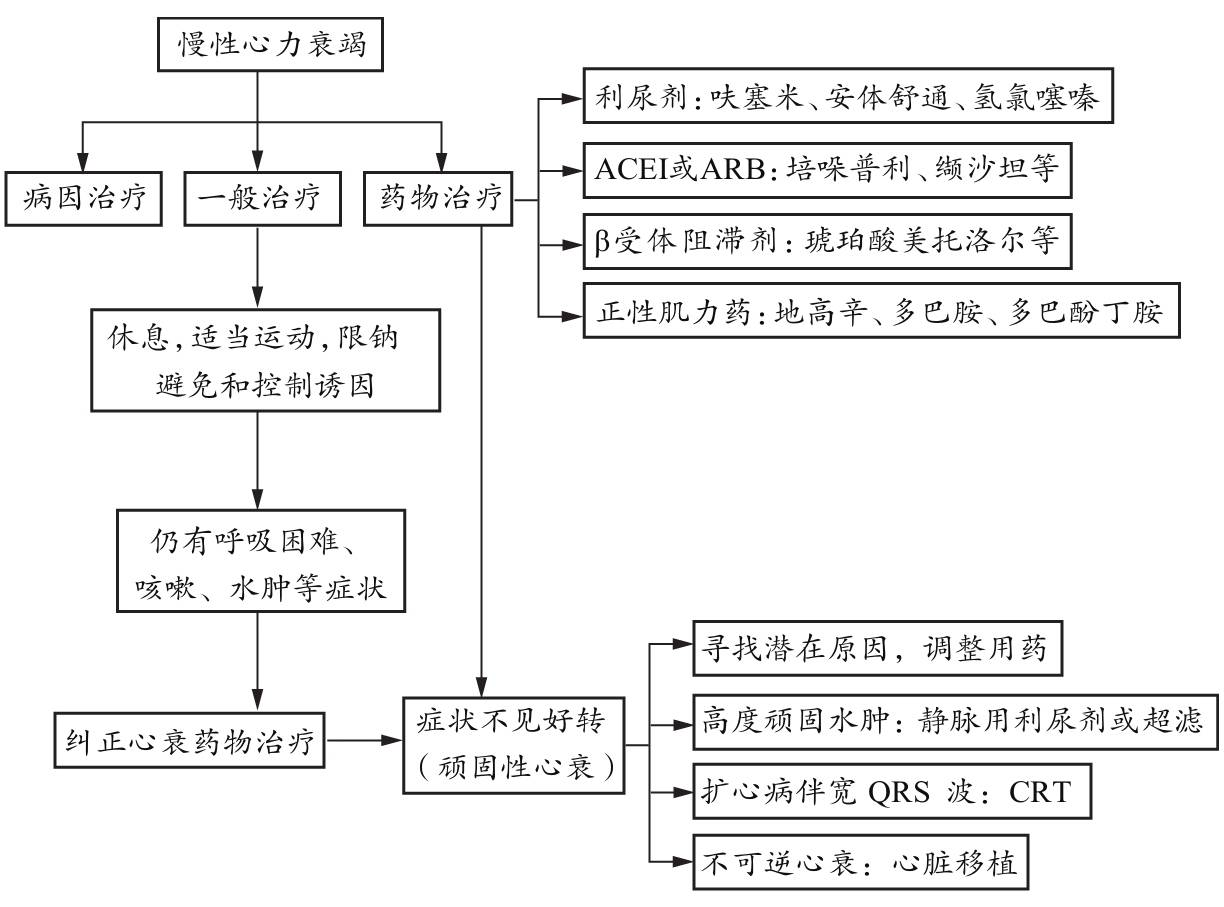
\includegraphics{./images/Image00043.jpg}
 \captionsetup{justification=centering}
 \caption{慢性心力衰竭的治疗程序}
 \label{fig2-1-1}
  \end{figure} 

【治疗方案】

{(一)病因治疗}

1.
基本病因治疗 如控制高血压、糖尿病等;药物、介入及手术治疗改善冠心病心肌缺血;慢性心瓣膜病以及先天畸形的介入或换瓣、纠治手术等;对于病因未明者如扩张型心肌病等,应从病理生理机制层面延缓或逆转心室重塑。

2.
消除诱因 控制感染、控制心房颤动的心室率、治疗甲状腺功能亢进、纠正贫血及水电解质紊乱。

3. 改善症状 “强心、利尿、扩血管,吗啡、激素、氨茶碱”。

4.
改善预后 在利尿剂基础上,加用神经内分泌抑制剂,如ACEI,或不能耐受ACEI加用ARB类。

{(二)一般治疗}

1.
休息 控制体力活动,避免精神刺激,降低心脏的负荷。鼓励心衰患者主动运动,根据病情轻重不同,从床边小坐开始逐步增加症状限制性有氧运动,如散步等。

2. 控制钠盐摄入。

{(三)药物治疗}

1.
利尿剂的应用 对慢性心衰患者原则上利尿剂应长期维持,水肿消失后,应以最小剂量无限期维持使用,该法不必加用钾盐。但是不能将利尿剂作单一治疗。常用的利尿剂包括:

(1)襻利尿剂:如呋噻咪(速尿)口服用20mg,2\textasciitilde{}4小时达高峰。对重度慢性心衰者用量可增至100mg,每日2次。托拉噻咪10mg,每日1\textasciitilde{}2次口服。效果不佳者可用静脉注射,每次用量100mg,每日2次,注意补钾。

(2)噻嗪类利尿剂:如氢氯噻嗪(双氢克尿噻)开始25mg,每日1次,逐渐加量。对较重患者用量可增至每日75\textasciitilde{}100mg,分2\textasciitilde{}3次服用,同时补充钾盐。

(3)保钾利尿剂:常用螺内酯(安体舒通)20mg,每日1次,一般与排钾利尿剂联合应用。

2. 肾素-血管紧张素-醛固酮系统抑制剂

(1)血管紧张素转换酶抑制剂:如培哚普利4\textasciitilde{}8mg,每日1次;卡托普利(Captopril)12.5\textasciitilde{}25mg,每日2次。

(2)血管紧张素受体阻滞剂:如缬沙坦(Valsartan)80\textasciitilde{}160mg,每日1次。

(3)醛固酮受体拮抗剂的应用:如螺内酯20mg,每日1次。

3.
β受体阻滞剂的应用 小剂量起始,如美托洛尔11.875mg/d、比索洛尔(Bisoprolol)1.25mg/d、卡维地洛6.25mg/d,逐渐增加剂量,以靶剂量或最大耐受量长期维持。

4. 正性肌力药

(1)洋地黄类药物:如地高辛,每日0.125\textasciitilde{}0.25mg。70岁以上或肾功能不良患者宜减量;或毛花苷C,为静脉注射用制剂,注射后10分钟起效,1\textasciitilde{}2小时达高峰,每次0.2\textasciitilde{}0.4mg稀释后静脉注射,24小时总量0.8\textasciitilde{}1.2mg,适用于急性心衰或慢性心衰加重时,特别适用于心衰伴快速心房颤动者。

(2)非洋地黄类正性肌力药:多巴胺2\textasciitilde{}5μg/(kg·min)静脉维持滴注,增加利尿效果;或米力农50μg/kg稀释后静脉注射,继以0.375\textasciitilde{}0.75μg/(kg·min)静脉滴注维持。

{(四)舒张性心功能不全}

1.
β受体阻滞剂 如美托洛尔11.875mg/d、比索洛尔1.25mg/d、卡维地洛6.25mg/d,逐渐增加剂量。

2.
钙通道阻滞剂 降低心肌细胞内钙浓度,改善心肌舒张功能,主要用于肥厚型心肌病。

3.
ACEI 如卡托普利12.5\textasciitilde{}25mg,每日2次;或培哚普利4\textasciitilde{}8mg,每日1次。

4.
保证心室舒张功能 尽量维持窦性心律,保持房室顺序传导,以保证心室舒张期充分容量。

5.
对肺淤血症状明显者 适量应用静脉扩张剂(硝酸盐类)或利尿剂降低前负荷,但过度减少前负荷可导致心排血量下降。

{(五)“顽固性心力衰竭”及不可逆心力衰竭的治疗}

1.
顽固性心力衰竭 积极寻找潜在病因、诱因,并尽可能纠正,如风湿活动、感染性心内膜炎、贫血、甲状腺功能亢进、电解质紊乱、洋地黄类过量、反复发作的肺栓塞等,患者是否并存其他非心血管疾病如肿瘤等。调整心衰治疗用药,加强效利尿剂、血管扩张制剂及正性肌力药物联合应用等。对高度顽固水肿也可使用血液滤过或超滤,超滤速度及有关参数调节恰当时,可获得即时显效。扩张型心肌病伴有QRS波\textgreater{}150ms者,可实施心脏再同步化治疗(cardiac
resynchronization
therapy,CRT),安置三腔心脏起搏器使左、右心室恢复同步收缩,有助于改善心衰症状及其预后。

2.
终末期慢性心衰 在常规药物、器械治疗基础上,考虑心脏辅助装置、心脏移植。

【疗效观察与随访】

1.
观察指标 临床症状、体征(肝大、肝颈反流试验阳性、水肿)、心电图、心功能、尿常规、X线胸片等。

2.
疗效评估 显效:呼吸平稳,心律规整、水肿消失,症状显著减轻。好转:症状体征减轻,但仍时有下肢水肿、肝肿大等。

3. 随访 定期复查心电图、尿常规,密切观察病情变化。

【治疗经验与解析】

1.
电解质紊乱是长期使用利尿剂最容易出现的不良反应,特别是高血钾或低血钾均可导致严重后果,应注意监测。ACEI、ARB等有保钾作用,与利尿剂合用时应注意监测血钾变化。血钠过低时,应区别是稀释性低钠血症还是体内钠量绝对不足,前者常表现为难治性水肿,水钠均有潴留,以水潴留为主。患者尿少而比重低,严重者可出现水中毒,可试用糖皮质激素。体内钠不足多因利尿过度所致,患者血容量减低,尿少而比重高,应给予高渗盐水补充钠盐。

2.
ACEI的不良反应有低血压、一过性肾功能恶化、高血钾及干咳。其禁忌证包括无尿性肾衰竭、妊娠哺乳期妇女及对ACEI过敏者。双侧肾动脉狭窄、血肌酐水平明显升高(\textgreater{}225μmol/L)、高血钾(\textgreater{}5.5mmol/L)及低血压者亦慎用。ARB的不良反应与ACEI相似,干咳发生率相对低。

3.
β受体阻滞剂具有负性肌力作用,临床应在干性心衰情况下应用,其应用原则从小量开始,逐渐增加剂量,最后靶剂量长期维持。

4.
在利尿剂、ACEI(或ARBs)和β受体阻滞剂治疗基础上心衰症状仍未缓解者,考虑加用地高辛。不同病因导致的心力衰竭对洋地黄的治疗反应不同。洋地黄对心腔扩大、舒张末期容积明显增加的慢性充血性心力衰竭效果较好。伴有心房颤动的心衰是应用洋地黄的推荐指征。代谢异常导致的高排血量心衰,如贫血性心脏病、甲状腺功能亢进及心肌炎、心肌病等所致的心衰,洋地黄治疗效果欠佳。肺源性心脏病导致右心衰,常伴低氧血症,洋地黄效果不佳且易导致洋地黄中毒,临床上应慎用。肥厚型心肌病主要是心肌舒张不良,增加心肌收缩性可能加重血流动力学障碍,因此,洋地黄属于相对禁忌。

5.
心衰患者的心肌处于血液或能量供应不足状态,过度或长期应用正性肌力药物将扩大能量的供需矛盾,使心肌损害更为加重,而导致死亡率增高。

6.
从建立心衰的分级、分期的观念为出发点,其治疗应包括防止和延缓心衰的发生;缓解临床心衰患者的症状,改善其长期预后和降低死亡率。采取综合治疗措施,包括对各种导致心功能受损的危险因素如冠心病、高血压、糖尿病的早期治疗;调节心衰的代偿机制,拮抗神经内分泌体液因子的过分激活,阻止心肌重构进展;对临床心衰患者,除缓解症状外,还应提高运动耐量,改善生活质量,阻止或延缓心肌损害进一步加重,降低死亡率。


\subsection{急性心力衰竭}

急性心力衰竭(acute heart
failure,简称急性心衰)是指急性的心脏病变引起心肌收缩力明显降低,或心室负荷加重而导致心排血量显著、急剧降低,体循环或肺循环压力突然增高,导致组织器官灌注不足和急性肺淤血的临床表现。临床上以急性左心衰竭最常见,表现为急性肺水肿,重者伴心源性休克。急性右心衰竭较少见,可发生于急性右心室梗死,或由大面积肺梗死引起的急性肺源性心脏病。

【治疗程序】 图\ref{fig2-1-2}所示。

\begin{figure}[!htbp]
 \centering
 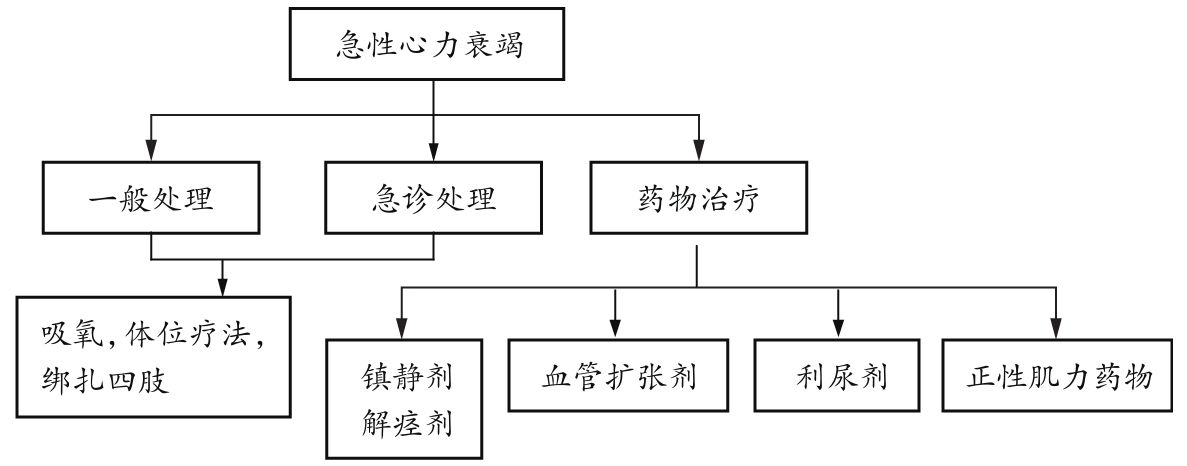
\includegraphics{./images/Image00044.jpg}
 \captionsetup{justification=centering}
 \caption{急性心力衰竭的治疗程序}
 \label{fig2-1-2}
  \end{figure} 

【治疗方案】

{(一)病因治疗和一般处理}

1.
体位 取坐位,双腿下垂,以减少静脉回心血量,降低心脏前负荷,有助于缓解心衰症状。

2.
吸氧 开始氧流量为每分钟2\textasciitilde{}3L,也可高流量给氧,必要时面罩加压给氧或正压呼吸。

3. 病因和诱因治疗 积极控制原发病和去除诱发或加重因素。

{(二)急诊处理}
 急性左心衰处理必须刻不容缓,立即给氧、使用正性肌力药物利尿剂,详见药物治疗。

{(三)药物治疗}

1.
对症治疗 如伴有疼痛,宜给予镇痛、镇静药物如吗啡:一般3\textasciitilde{}5mg静脉注射,必要时每隔15分钟重复1次,共2\textasciitilde{}3次,或5\textasciitilde{}10mg皮下注射或肌内注射。

2.
治疗药物 对于急性收缩性心力衰竭,给予有效缓解心力衰竭症状的药物。①襻利尿剂,如呋塞米20\textasciitilde{}40mg静脉推注,短期内具有血管扩张作用,而后产生利尿作用,从而有效缓解心衰症状。②正性肌力药物,其中包括洋地黄制剂,如毛花苷C0.2\textasciitilde{}0.4mg静脉推注,必要时2\textasciitilde{}4小时可重复给药。③血管扩张剂,对于各种原因引起的急性肺水肿均有良好疗效,首选药物为硝普钠,初始量每分钟10\textasciitilde{}15μg,在严密观察下逐渐增量至每分钟50\textasciitilde{}100μg;如肺水肿并低血压或休克时,可用硝普钠和多巴胺或多巴酚丁胺联合静脉滴注。

3.
其他药物 氨茶碱可解除支气管痉挛、减轻呼吸困难、正性肌力、扩张外周血管和利尿,常用剂量0.25g稀释后滴注;糖皮质激素的应用。

{(四)介入和其他治疗措施}
 电复律、主动脉内球囊反搏、机械通气、血液净化等。

【疗效观察与随访】

1.
观察指标 水肿、肺部湿啰音、端坐呼吸、颈静脉怒张、肝肿大、肝颈逆流征、心功能、心电图、床边X线胸片等。

2.
治愈标准 临床症状、体征消失、呼吸平稳、心功能纠正等。好转标准:心功能改善,但未达到Ⅰ级,呼吸困难改善,但夜间平卧仍较困难。

3.
随访 密切观察病情变化,注意有无再心衰,定期复查心电图、心功能,定期听诊心肺,特别注意原发病未解除者,再发心衰较常见。

【治疗经验与解析】

1.
急性心衰经初步急诊处理后,及早确定诱因并给予治疗。有高血压危象者应适当降压,选用硝普钠;器质性心脏病如急性心肌梗死应及早血运重建;快速型心律失常对药物无效,而非洋地黄引起,应迅速电复律等。

2.
对基本病因和基础心脏病做出诊断:如重度二尖瓣狭窄、感染性心内膜炎伴瓣膜穿孔及肥厚梗阻性心肌病等,应给予相应处理。


\section{心律失常}

心脏电活动起源于窦房结,经过扩布后引起心脏持续规律地收缩和舒张。窦房结的冲动先扩布到右、左心房,然后到达房室结,沿着房室束及左右束支、普肯耶纤维网传导激动心室肌,使得心房和心室顺序收缩和舒张,是为窦性心律。成人正常窦性心律时心率一般为60\textasciitilde{}100次/分,较规则。心律起源(部位、频率与节律)和传导(速度、时间、途径、顺序)等任一项异常均称为心律失常。

心律失常可按发生原理、起源部位、心律失常时心率的快慢,以及心律失常时循环障碍的严重程度和预后分类。按发生原理,心律失常可分为自律性异常、折返形成、后除极触发、传导异常以及上述异常的联合。按起源部位,则可分为窦性、心房性、房室结性、房室交界性和心室性,总称为室上性与室性心律失常。按心律失常时心率的快慢,分为快速和缓慢性心律失常。有些学者还提出按心律失常时循环障碍的严重程度和预后,将心律失常分为良性和恶性两大类,或分为致命性、潜在致命性和良性三类。

心律失常可见于各种器质性心脏病,其中以冠状动脉粥样硬化性心脏病(简称冠心病)、心肌病、心肌炎和风湿性心脏病(简称风心病)为多见,尤其在发生心力衰竭或心肌梗死时。发生在基本健康或者自主神经功能失调患者中的心律失常也常见。其他病因有电解质或内分泌失调、麻醉、低温、胸腔或者心脏手术、药物作用和中枢神经系统疾病等。部分病因不明。

\subsection{窦性心律失常}

{(一)窦性心动过速、窦性心动过缓}
 窦性心动过速即窦性心律频率在成人超过100次/分。窦性心动过缓指窦性心律频率低于60次/分。窦性心动过缓见于10\%\textasciitilde{}15\%的急性心肌梗死患者,主要为下壁心肌梗死的早期,溶栓治疗后再灌注时,也可出现窦性心动过缓。慢性不适宜的窦性心动过速或慢性非阵发性窦性心动过速可见于正常人,可能由于窦房结自律性增高或窦房结邻近存在自律性心房起搏点,交感或迷走神经对窦房结自律性调节失控所致。亦见于房室结心动过速射频消融术后。心电图特征:窦性P波,PR间期≥0.12s而\textless{}0.20s,窦性心动过速时PP间距短于0.6s,窦性心动过缓时PP间期长于1.0s。

窦性心动过速,见图\ref{fig2-2-1}。
\begin{figure}[!htbp]
    \centering
    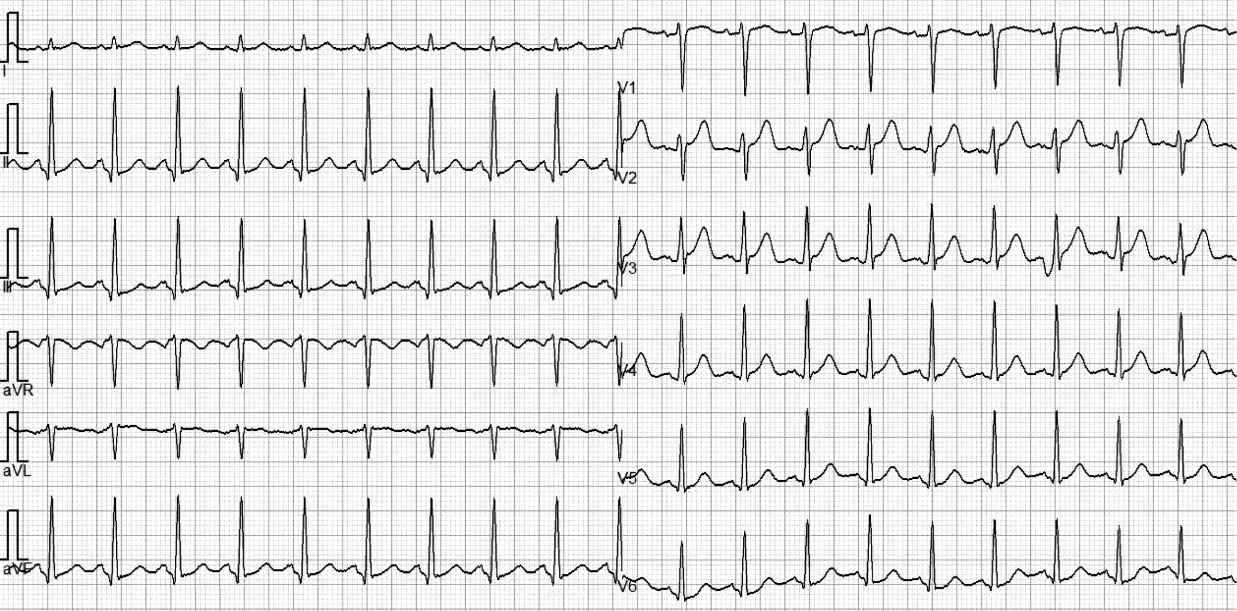
\includegraphics[
        height=.3\textheight,
        width=\textwidth,
        keepaspectratio]{./images/Image00045.jpg}
    \captionsetup{justification=centering}
    \caption{窦性心动过速}
    \label{fig2-2-1}
\end{figure}

窦性心动过缓,见图\ref{fig2-2-2}。

\begin{figure}[!htbp]
 \centering
 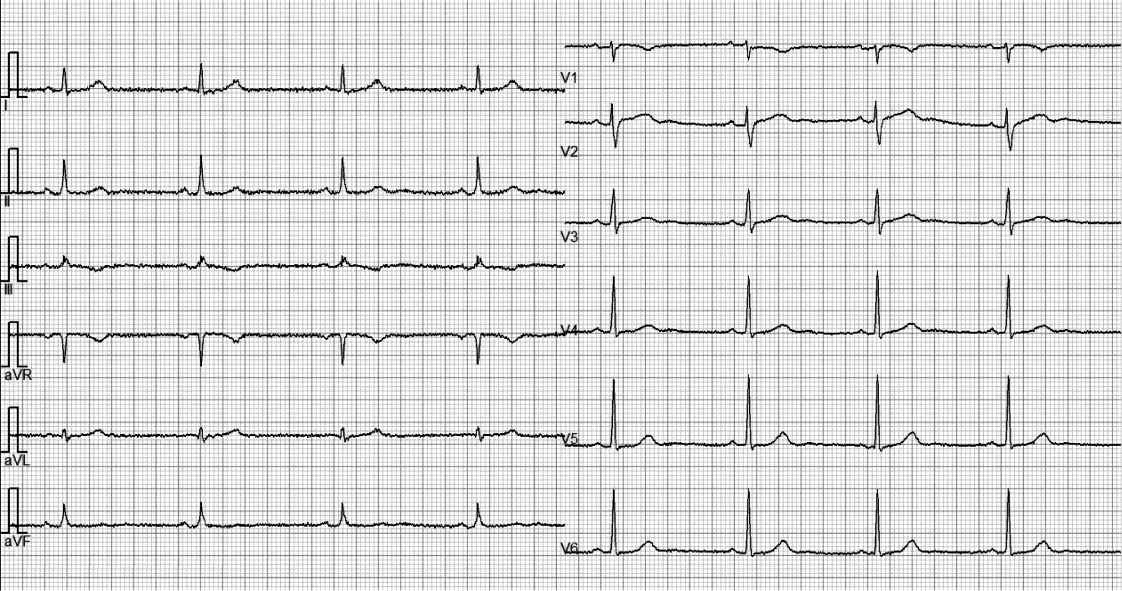
\includegraphics[
    height=.3\textheight,
    width=\textwidth,
    keepaspectratio]{./images/Image00046.jpg}
 \captionsetup{justification=centering}
 \caption{窦性心动过缓}
 \label{fig2-2-2}
\end{figure} 

【治疗方案】

1.
窦性心动过速 无症状性窦性心动过速一般无需治疗,有症状者应行病因治疗和去除诱因。在排除禁忌证后,必要时考虑使用β受体阻滞剂(如美托洛尔、阿替洛尔)、非二氢吡啶类钙离子拮抗剂(如硫氮䓬
酮),或镇静剂(如地西泮)等。

2.
窦性心动过缓 无症状性窦性心动过缓一般无需治疗,有症状者应进行病因治疗和去除诱因,并酌情选用M受体阻断剂(如阿托品)、β受体激动剂(如异丙肾上腺素)或非特异性兴奋剂、传导促进剂,严重者(反复晕厥等)必要时行心脏起搏治疗。

【疗效观察与随访】 观察患者的心、脑、肾等脏器供血不足症状,尤其是脑供血不足症状,如乏力、头晕、记忆力差、反应迟钝有无改善,心电图异常有无纠正等。

【治疗经验与解析】

1.
对于窦性心动过速,除了生理状况外,重点需要排除甲状腺功能亢进、贫血等基础疾病,以及有无发热、应用肾上腺素、阿托品等病情。症状缓解后即可停药。

2.
对于窦性心动过缓,除了生理状况外,重点需要排除颅内疾患、甲状腺功能减退、严重缺氧、阻塞性黄疸等基础疾病,以及有无低温、应用拟胆碱药、胺碘酮、β受体阻滞剂、普罗帕酮、非二氢吡啶类钙通道阻滞剂或洋地黄药物等。药物治疗效果差时,考虑安装心脏起搏器。

{(二)窦房传导阻滞}
 窦房传导阻滞指窦房结发出的冲动在传至心房过程中发生的阻滞,简称窦房阻滞。常见病因包括冠心病、心肌病、心肌炎、家族性窦房结病、窦房结损伤(如房间隔缺损修补术中),洋地黄和奎尼丁等药物不良反应及各种原因引起的迷走神经张力增高等。临床表现除病因表现外,其症状取决于P波连续脱落次数和长PP间期的时限,轻者仅表现为头晕、乏力,重者发生晕厥。按严重程度可分为一度、二度和三度窦房阻滞。由于体表心电图不能显示窦房结电位,故不能明确诊断一度和三度窦房阻滞。二度窦房阻滞可分为以下类型:二度Ⅰ型窦房阻滞,其特点为一系列连续出现的P波中,PP间期逐渐缩短,直至发生一次P波脱漏,出现长的PP间期,其长PP间期小于短PP间期的2倍;二度Ⅱ型窦房阻滞特点为一系列连续出现的P波中,多数PP间期相等,间歇性发生P波脱漏,出现长的PP间期,其长PP间期等于短PP间期的2倍或整倍数。

【治疗方案】 参见病态窦房结综合征。

【疗效观察与随访】 无症状或症状轻者,需要注意患者的症状、体征,以及有无晕厥发生,监测心电图。

【治疗经验与解析】 无症状或症状轻者,需要定期复查心电图,有条件定期行动态心电图监测,一旦病情加重,如发生晕厥等,必须立即行心脏起搏治疗。

{(三)窦性静止}
 窦性静止指窦房结在一定时间内失去自律性、不能发放电冲动而引起的心律失常,又称窦性停搏。其病因包括冠心病、窦房结变形、颅内压增高,亦可由各种原因引起的迷走神经张力增高和某些药物(如洋地黄、β受体阻滞剂等抗快速心律失常药物、钾盐、乙酰胆碱)等所致。临床症状与相关病因症状、窦性停搏时限的长短有关,严重者可出现眩晕、黑矇、晕厥,甚至发生阿-斯综合征。心电图表现为较长时间内不出现P-QRS-T波群,长间歇内可能出现交界性或室性逸搏。

【治疗方案、疗效观察与随访及治疗经验与解析】 参见(二)窦房传导阻滞。

{(四)病态窦房结综合征}  病态窦房结综合征(sick sinus
syndrome,SSS)简称病窦综合征,由窦房结及其邻近组织病变引起窦房结起搏功能和(或)窦房传导障碍,从而产生多种心律失常和临床症状。多在40岁以后出现症状。常见病因包括心肌病、冠心病、心肌炎、结缔组织病、代谢或浸润性疾病等,仍有病因未明者。该病病程发展大多缓慢,少数急性起病,见于急性心肌梗死和急性心肌炎。

临床表现轻重不一,可呈间歇发作性。多以心率缓慢所致脑、心、肾等脏器血供不足尤其脑供血不足症状为主。轻者乏力、头晕、眼花、失眠、记忆力差、反应迟钝或易激动等,严重者可有短暂黑矇、近乎晕厥或阿-斯综合征发作。部分患者合并短阵室上型快速心律失常发作,又称慢快综合征。心动过速突然中止后可有心脏暂停(伴或不伴晕厥)。严重心动过缓或心动过速除引起心悸外,还可加重原有心脏病症状,引起心力衰竭或心绞痛。心排量过低严重影响肾脏等脏器灌注,导致少尿、消化不良等。慢快综合征还可能导致血管栓塞。

【治疗程序】 见图\ref{fig2-2-3}所示。

\begin{figure}[!htbp]
 \centering
 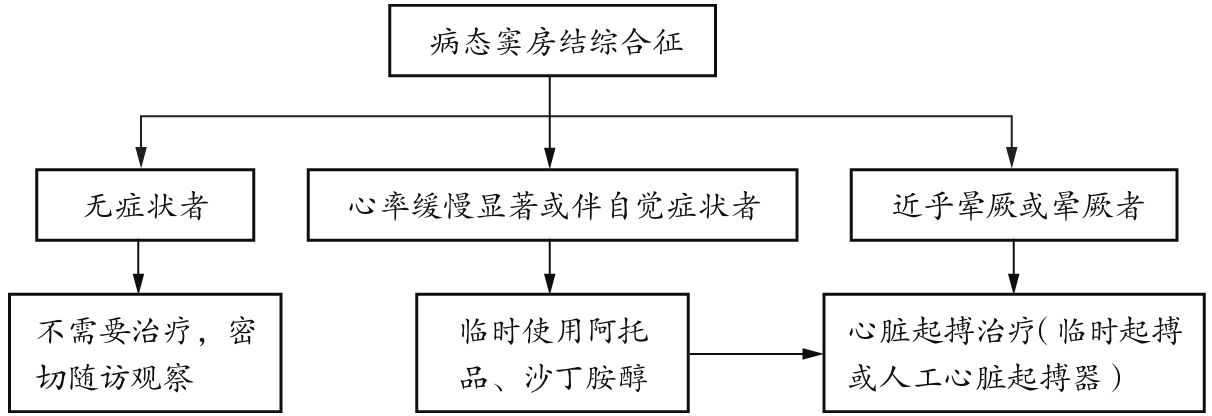
\includegraphics{./images/Image00048.jpg}
 \captionsetup{justification=centering}
 \caption{病态窦房结综合征的治疗程序}
 \label{fig2-2-3}
  \end{figure} 

【治疗方案】 治疗应针对病因,无症状者可定期随访,密切观察病情。心率缓慢显著或伴自觉症状者可临时使用阿托品、沙丁胺醇(舒喘灵)口服。双结病变、慢快综合征以及明显脑供血不足症状如近乎晕厥或晕厥的患者,建议植入按需型人工心脏起搏器,房室顺序按需起搏器,较ⅤⅥ型起搏器更符合生理要求并减少血栓栓塞风险。合并快速心律失常者,安装起搏器后再加用药物控制快速心律失常发作。在无起搏器保护下,病窦综合征患者禁用减慢心率药物。

【疗效观察与随访】 观察患者的症状、体征,对于无症状者,需要经常监测心电图、动态心电图;如果心动过缓显著,伴脑缺血症状,需要立即予药物或心脏起搏治疗,尤其是R-R间歇\textgreater{}2.5秒时。

【治疗经验与解析】

1.
R-R间歇\textgreater{}2.5秒,伴心源性脑缺血症状时,需要立即安装人工心脏起搏;R-R间歇≤2.5秒时,需要密切随访,可不安装人工心脏起搏器,但积极安装亦可行。

2.
应尽量选择近似生理性起搏器,如AAI或DDD,并通过程控减少心室起搏的比例,从而减少心房颤动和血栓栓塞的危险。

3.
病窦综合征患者有心房颤动或心房扑动发作时,不宜进行电复律,除非已植入起搏器。

4.
安装人工心脏起搏器后,药物治疗仍不满意的心房颤动、心房扑动或房性心动过速等快速型心律失常患者,应采取个体化治疗。即如果严重窦性心动过缓和窦性停搏只出现在心房颤动、心房扑动或房性心动过速终止后,可首先行导管消融治疗心房颤动及其他快速性心律失常,然后根据随访中心动过缓的情况评价心脏起搏治疗的必要性。

\subsection{房性心律失常}

{(一)房性期前收缩}
 起源于心房的期前收缩称为房性期前收缩,简称房早。房早可见于健康人,尤其健康老年人,也可由其他相关疾病引起,如风湿性心脏病二尖瓣病变、冠心病、高血压病、甲状腺功能亢进和低钾血症等。临床表现除病因相关表现外,多无明显症状,部分患者可有心悸、胸闷、恶心不适等。心脏听诊时,期前收缩第一心音增强,第二心音减弱或消失,其后有一段较长间期。心电图表现为提前出现的P'{-}QRS-T波群,P'R间期≥120ms,QRS通常为室上型,不完全代偿(图\ref{fig2-2-4})。

\begin{figure}[!htbp]
 \centering
 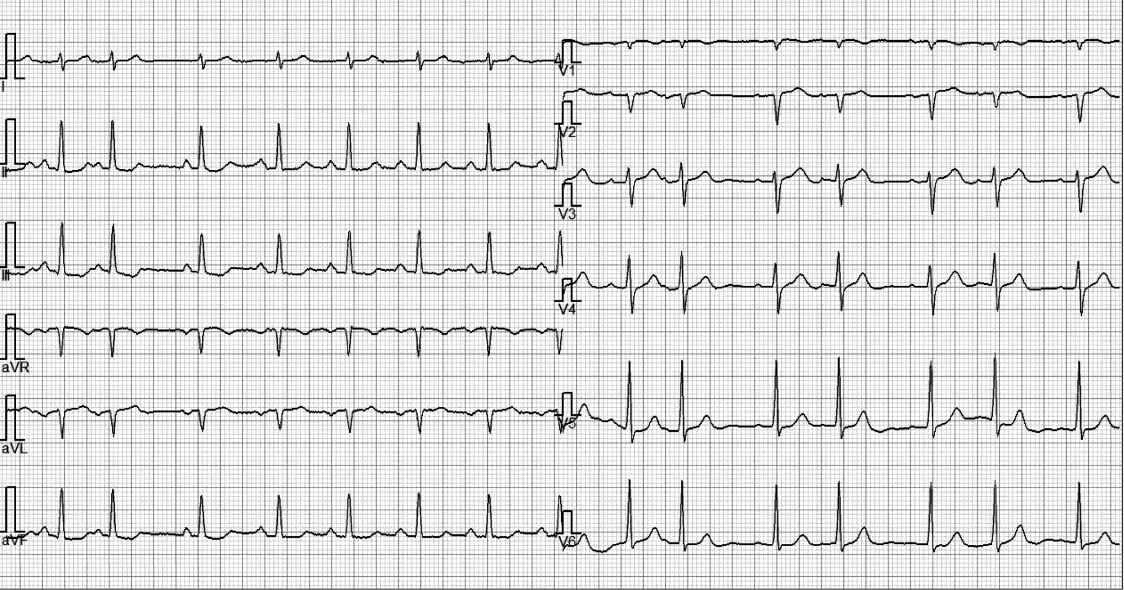
\includegraphics[
    height=.3\textheight,
    width=\textwidth,
    keepaspectratio]{./images/Image00049.jpg}
 \captionsetup{justification=centering}
 \caption{房性期前收缩}
 \label{fig2-2-4}
  \end{figure} 

【治疗程序】 图\ref{fig2-2-5}所示。

\begin{figure}[!htbp]
 \centering
 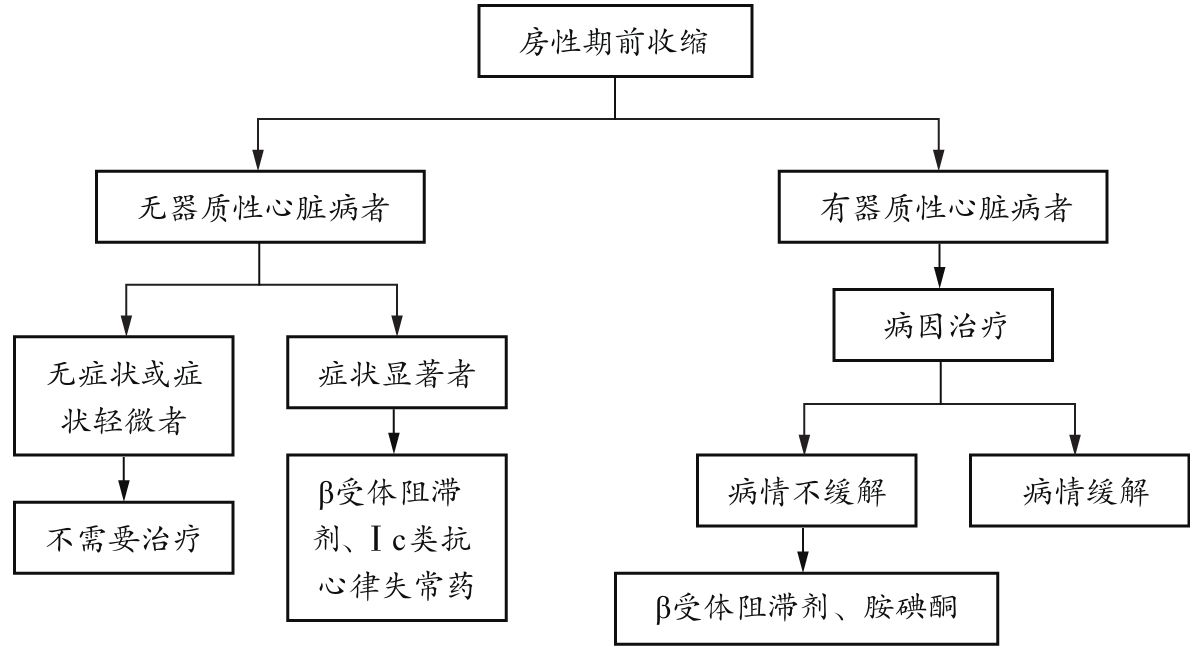
\includegraphics{./images/Image00050.jpg}
 \captionsetup{justification=centering}
 \caption{房性期前收缩的治疗程序}
 \label{fig2-2-5}
  \end{figure} 

【治疗方案】 无器质性心脏病者一般无需治疗,症状显著者可考虑使用β受体阻滞剂、Ⅰc类抗心律失常药物等,由紧张过度、情绪激动或运动诱发的,可试用镇静剂和β受体阻滞剂;伴有器质性心脏病的房性早搏患者,随着病因治疗和病情缓解后房早多能减少或消失,不主张长期用抗心律失常药物;对房早诱发室上性心动过速或心房颤动者,可选用β受体阻断剂、Ⅰc类抗心律失常药、莫雷西嗪或维拉帕米等。

【疗效观察与随访】 评估患者的精神状态,有无器质性心脏病,症状与房性期前收缩的相关性,监测治疗前后的心电图、动态心电图等变化。

【治疗经验与解析】 本病一般无需治疗,伴有心衰和心肌梗死患者禁用Ⅰc类抗心律失常药。若应用抗心律失常药治疗,应注意根据症状以及心电图转归,症状缓解后予减量治疗,并适时停药。

{(二)房性心动过速}
 连续发生3个或3个以上的房早称为房性心动过速,简称房速。按发生机制分为房内折返性心动过速(IART)、房内自律性心动过速(AAT)和房性紊乱性心动过速(CAT)等(图\ref{fig2-2-6})。

\begin{figure}[!htbp]
 \centering
 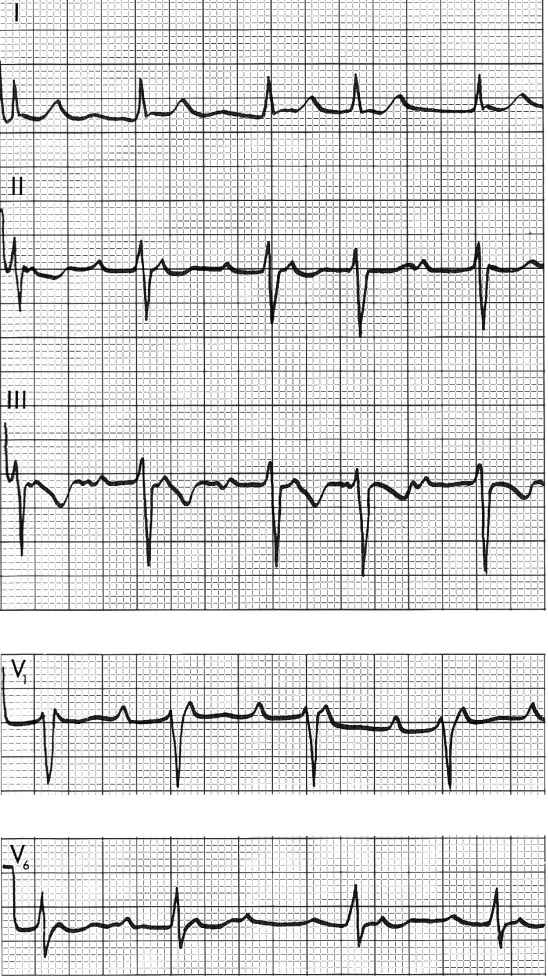
\includegraphics[
    height=.5\textheight,
    width=\textwidth,
    keepaspectratio]{./images/Image00051.jpg}
 \captionsetup{justification=centering}
 \caption{房性心动过速}
 \label{fig2-2-6}
  \end{figure} 

1.
IART多见于器质性心脏病伴心房肥大、心肌病、心肌梗死、低钾血症和洋地黄中毒等患者。除病因相关表现外,IART常反复发作,发作时有心悸、气促和胸闷等,一般无明显严重症状和血流动力学障碍。心电图表现为房性P'波频率130\textasciitilde{}150次/分,偶可高达180次/分,较为规则;P'波形态与窦性P波形态不同,与房内折返途径相关;P'R间期≥120ms,发生房室传导阻滞时不能终止发作。

2.
AAT发作时有胸闷、心悸、气促等症状,多不严重。洋地黄中毒者可致心力衰竭加重、低血压或休克等。AAT可间断发作,也可持续数月或数年,少数患者发展为“心动过速性心肌病”。心电图表现为房性P'波频率100\textasciitilde{}200次/分,发作初期频率渐趋稳定(温醒现象);P'波形态与窦性P波形态不同,与异位兴奋灶部位有关;P'R间期≥120ms,发生房室传导阻滞时不能终止发作。

3.
CAT发作时常诱发或加重心功能不全,易发展为心房颤动,部分患者提示预后不良。心电图表现为:房性P'波频率100\textasciitilde{}130次/分;有3种或3种以上的P'波,且P'波之间可见等位线;P'P'、P'R、RR间距不规则,部分P'波不能下传心室。

【治疗程序】 图\ref{fig2-2-7}所示。

\begin{figure}[!htbp]
 \centering
 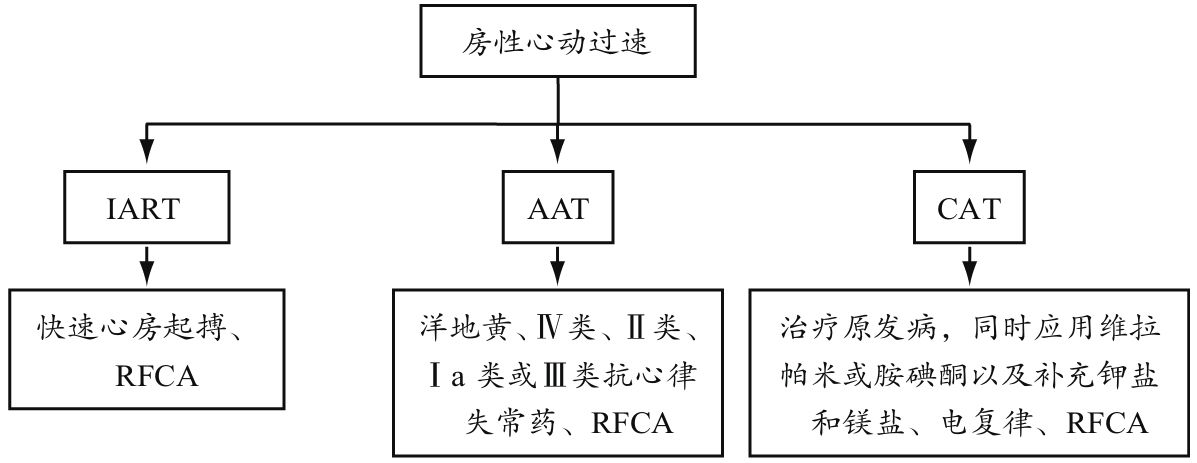
\includegraphics{./images/Image00052.jpg}
 \captionsetup{justification=centering}
 \caption{房性心动过速的治疗程序}
 \label{fig2-2-7}
  \end{figure} 

【治疗方案】

1.
IART 可通过快速起搏心房终止房性心动过速,射频消融术(RFCA)也有较高的成功率,但复发率较高,刺激迷走不能终止IART。

2.
AAT 可选用洋地黄、Ⅳ类、Ⅱ类、Ⅰa类或Ⅲ类抗心律失常药物。必要时行RFCA,心房起搏和刺激迷走神经方法不能终止AAT。RFCA效果较好。

3.
CAT 首先治疗原发疾病,同时应用维拉帕米或胺碘酮以及补充钾盐和镁盐。药物治疗无效或出现血流动力学改变,可选择或直接进行同步直流电复律,如条件和技术水平许可,亦可选择进行食管调搏复律。RFCA效果较好。

【疗效观察与随访】 观察治疗后患者的症状、体征以及心电图改变。

【治疗经验与解析】 RFCA是根治的最佳方案。

{(三)心房扑动和心房颤动}
 心房扑动(房扑)和心房颤动(房颤)在病因和发病机制上密切相关,有时可相互转化。

房颤是成人最常见的心律失常之一,较房扑多见,房扑和房颤均可呈阵发或持久发作,前者可反复短阵发作,后者则持续发作不止,阵发性房颤通常\textless{}7日(大多\textless{}24小时),可自行复律。持续性房颤\textgreater{}7日,不能自行终止,可药物或电复律,也可复发。持久性房颤\textgreater{}1年难以复律或复律后难以维持窦性心律。阵发性房扑或房颤长期反复发作,多数演变为持久性房颤。

房扑和房颤的症状与基础心脏病、心室率快慢和心房收缩对心室充盈量的影响程度有关。部分患者可无症状,通常发作时有心悸感,伴原有病情加重,如气促、心前区疼痛、运动耐量减低,甚至发生心衰、肺水肿等。房扑时心室率可随房室传导比例变化而显著变化,如静卧、颈动脉窦按摩时心室率显著下降,运动、情绪激动可使心室率显著增高。房扑通常不稳定,趋向于转为窦律或房颤。持续数月或数年者少见。房扑发作时心房收缩协调,其栓塞事件低于房颤。房颤时,心室率大多较快,心音强弱不等,节律完全不规则;心室率快时,脉搏短绌(脉率慢于心率)明显。少数房颤患者以栓塞并发症或晕厥为首发症状,晕厥多见于病态窦房结综合征、慢快综合征、肥厚型梗阻性心肌病、主动脉瓣狭窄并发房颤患者。

房扑时心电图示P波消失,代之以连续的、形状规则、大小一致的锯齿样波(F波),频率250\textasciitilde{}350次/分,多数心室率为心房率一半,在150次/分左右。房颤的心电图示P波消失,代之以形态不同、大小不等的不规则细小波形(f波),频率350\textasciitilde{}600次/分,心室节律绝对不规则。如图\ref{fig2-2-8}所示。

\begin{figure}[!htbp]
 \centering
 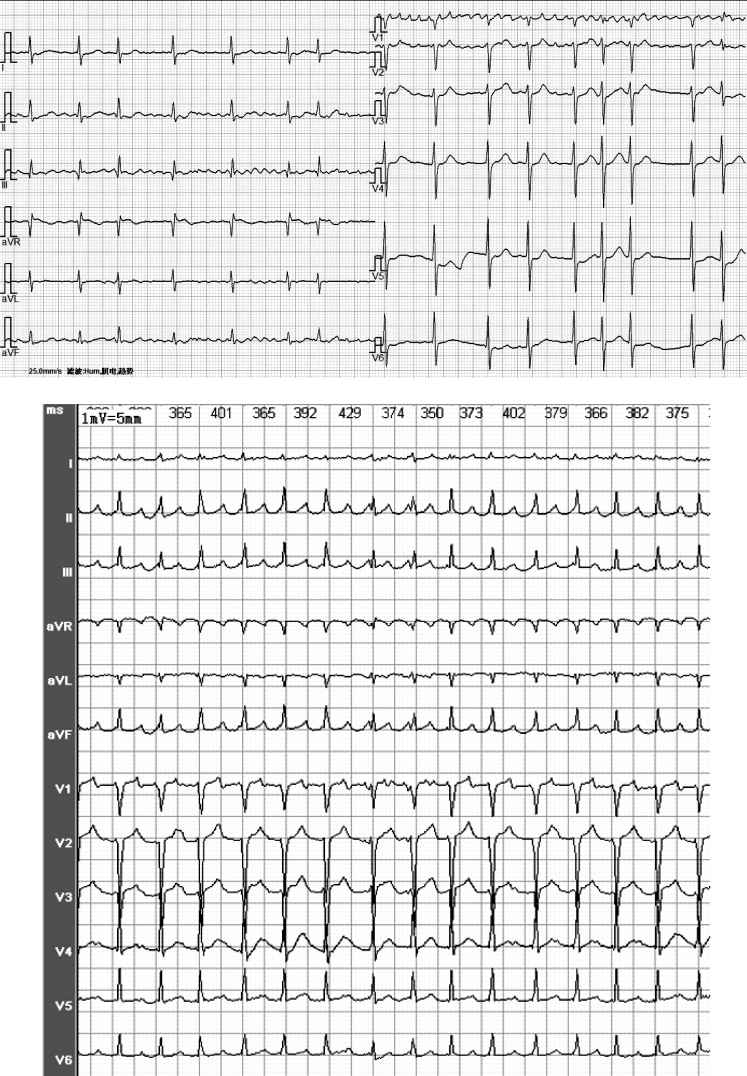
\includegraphics[
    height=.6\textheight,
    width=\textwidth,
    keepaspectratio]{./images/Image00053.jpg}
 \captionsetup{justification=centering}
 \caption{心房扑动和心房颤动}
 \label{fig2-2-8}
  \end{figure} 

【治疗程序】

1. 心房颤动阶梯式治疗程序 如图\ref{fig2-2-9}所示。

\begin{figure}[!htbp]
 \centering
 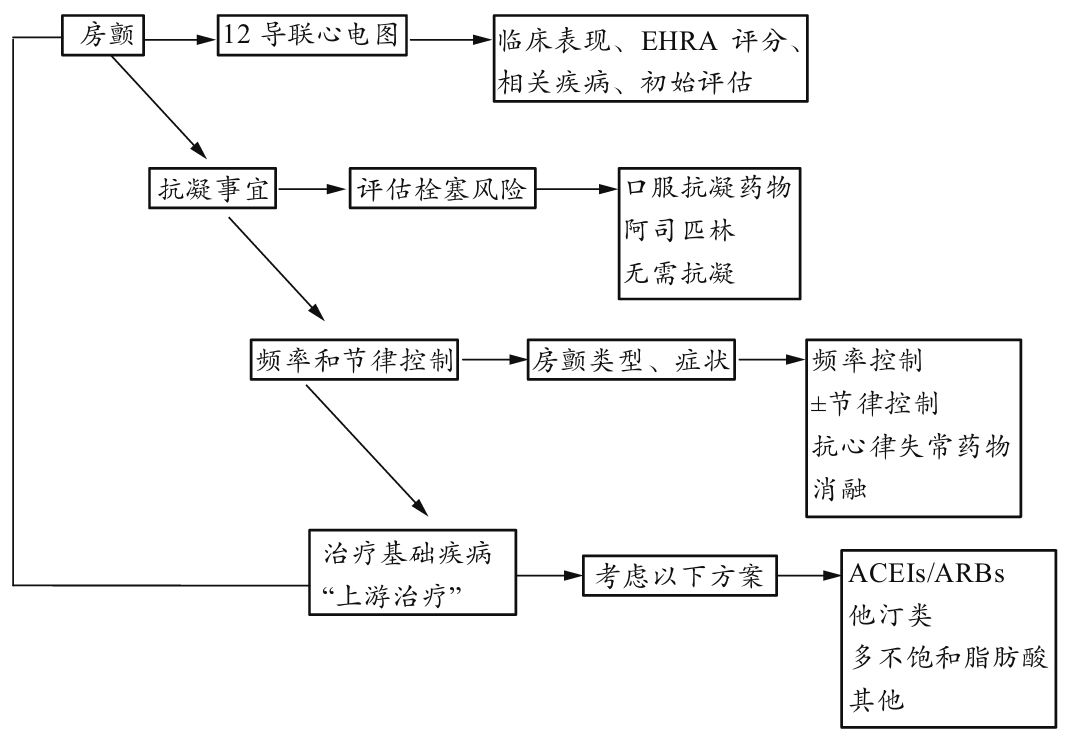
\includegraphics{./images/Image00054.jpg}
 \captionsetup{justification=centering}
 \caption{心房颤动阶梯式治疗程序}
 \label{fig2-2-9}
  \end{figure} 

2. 心房颤动的抗凝治疗 如图\ref{fig2-2-10}\footnote{*:其他危险因素包括:年龄65\textasciitilde{}74岁、女性、血管疾病。}所示。

\begin{figure}[!htbp]
 \centering
 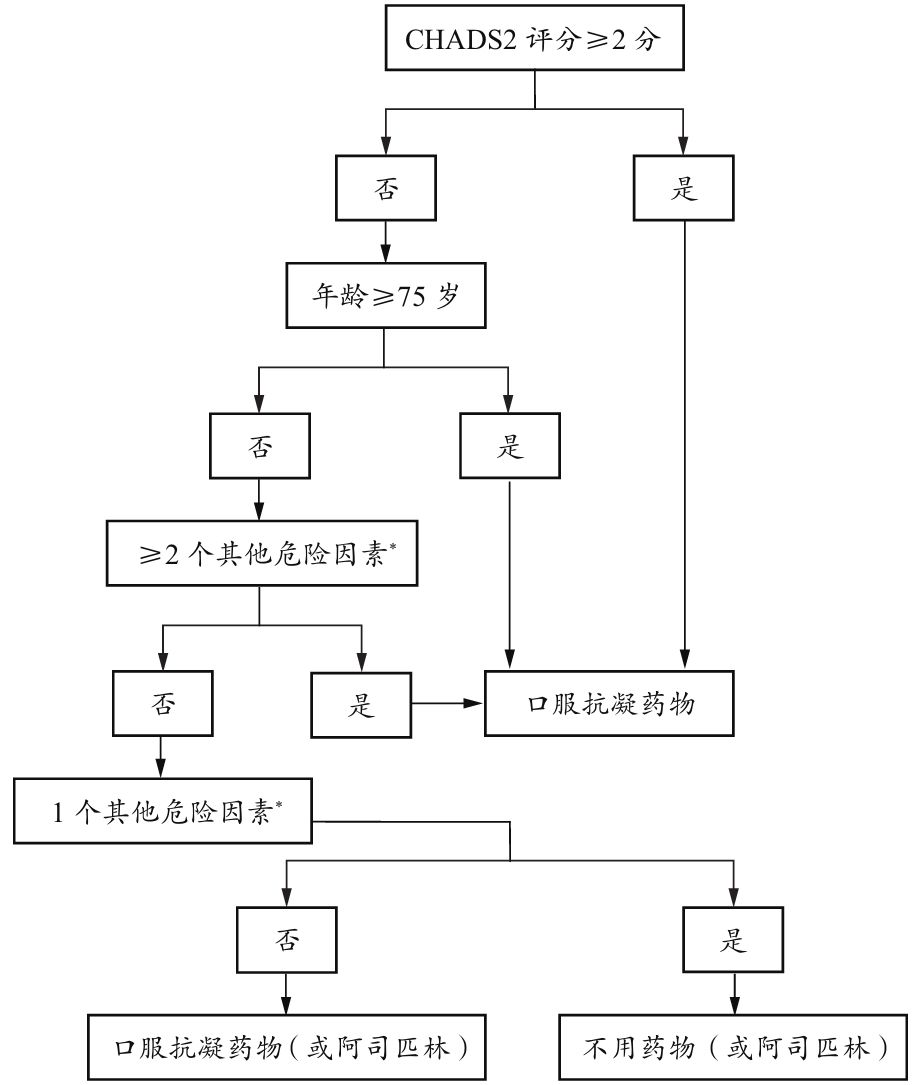
\includegraphics{./images/Image00055.jpg}
 \captionsetup{justification=centering}
 \caption{心房颤动患者抗凝方案}
 \label{fig2-2-10}
  \end{figure} 



3. 心房颤动患者药物治疗和导管消融选择 如图\ref{fig2-2-11}所示。

\begin{figure}[!htbp]
 \centering
 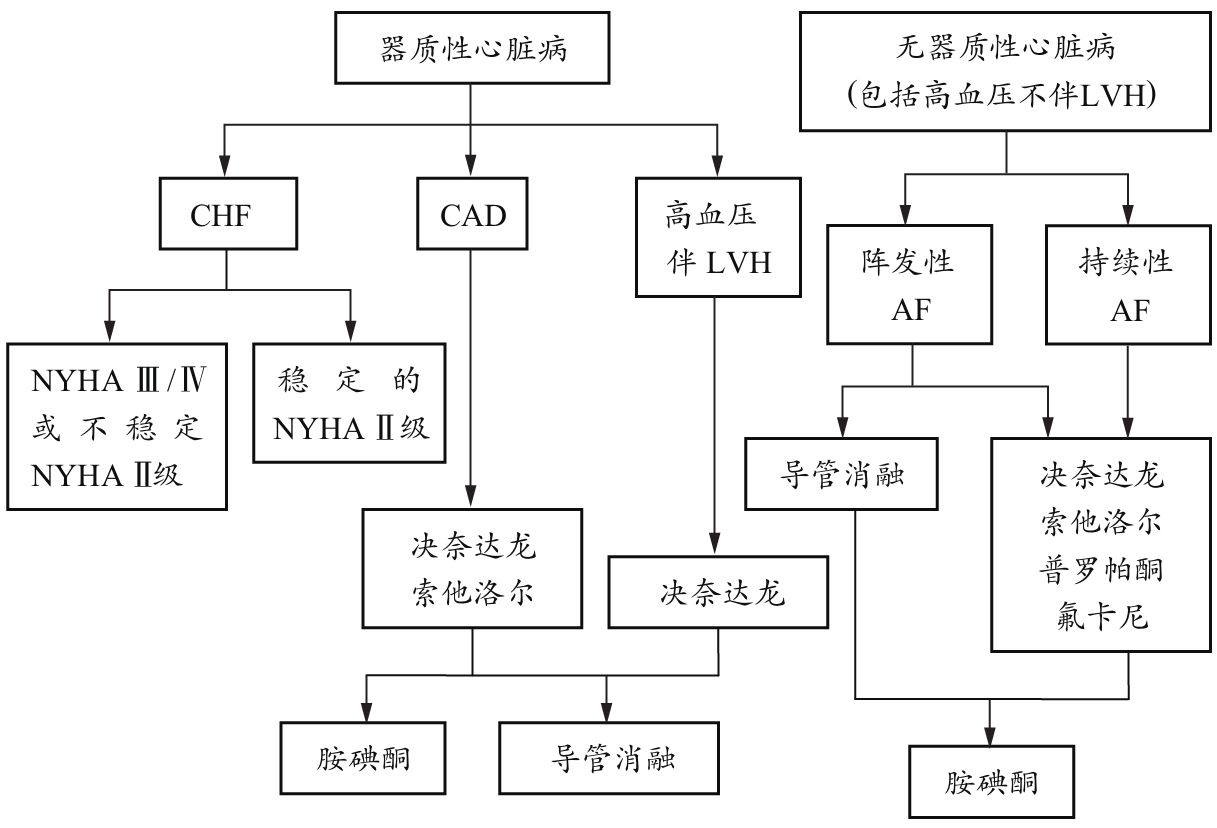
\includegraphics{./images/Image00056.jpg}
 \captionsetup{justification=centering}
 \caption{心房颤动患者药物治疗和导管消融选择}
 \label{fig2-2-11}
  \end{figure} 

【治疗方案】

1. 房速、房扑的治疗

(1)病因治疗:治疗原发病,如风湿性心脏病、冠心病、高血压心脏病和甲亢性心脏病等。

(2)转复心律:包括同步直流电复律、经食管心房调搏术、经导管射频消融术和药物复律等。

(3)控制心室率:通常首选非二氢吡啶类钙通道阻滞剂,伴有心衰患者首选洋地黄类,如无禁忌亦可选用β受体阻滞剂,必要时联合用药。

(4)抗凝治疗:血栓栓塞高危人群,应考虑抗凝治疗,通常选用华法林,控制PT-INR
2\textasciitilde{}3。

2. 房颤治疗

(1)病因治疗:同房速、房扑的治疗。

(2)防治血栓栓塞:房颤患者为血栓栓塞高危人群,抗凝治疗很重要。治疗前应评估房颤患者发生血栓栓塞风险,2010年ESC公布新的评估标准,即CHA2DS2-VASc评分:包括心力衰竭、高血压、年龄≥75岁,糖尿病、中风/TIA/血栓栓塞、血管疾病、年龄65\textasciitilde{}74岁、女性等,其中年龄≥75岁及中风/TIA/血栓栓塞评分为2分,其余均为1分。CHA2DS2-VASc评分≥2分时,需服用抗凝剂如华法林抗凝,1分可选用阿司匹林,0分者可不用抗凝药物或抗血小板治疗。

(3)控制心室率:常用药物有洋地黄类、β受体阻滞剂、非二氢吡啶类钙通道阻滞剂等。2010年ESC指南建议,心室率控制在静息时80次/分,轻微运动时不超过100次/分,无症状者可放宽至静息时≤110次/分。控制心室率时要求兼顾患者长间歇,应在动态心电图指导下进行,若患者有长间歇(尤其RR间期≥5秒),必要时在起搏器保护下进行。

(4)转复窦性心律:适用于年龄较轻、房颤病史短于1年、发作时症状较重、左房内径\textless{}45mm和无器质性心脏病等患者。复律手段有4种,即药物复律、同步电复律、经导管射频消融术(RFCA)及外科迷宫手术。无器质性心脏病患者,可选Ⅰa及Ⅰc类药物复律,器质性心脏病患者宜选用胺碘酮。同步治疗电复律通常适用于快速房颤伴有血流动力学障碍患者及药物复律失败者,病态窦房结综合征患者禁忌同步电复律。RFCA主要应用肺静脉隔离方式,目前成功率80\%\textasciitilde{}90\%,具有良好前景。外科迷宫手术通常与需矫正心脏结构手术同时进行。

(5)上游治疗:近年提出的新理念,某种程度上为病因治疗,包括ACEIs/ARBs、他汀类药物、多不饱和脂肪酸等。

【疗效观察与随访】

1.
抗凝是否达标 服用华法林抗凝者,PT-INR通常在2\textasciitilde{}3,低于下限抗凝不充分,血栓栓塞风险增大,需加大华法林剂量;高于上限者,出血风险增大,需减量、停药,必要时使用维生素K{1}
拮抗。

2.
常规12导联心电图或动态心电图监测心率及心律 控制心室率应根据动态心电图监测及调整药物,通常要求房颤患者休息时心室率70次/分左右,轻微运动时不超过90次/分。转复窦律治疗患者,若多次尝试药物转复而失败者,可尝试射频消融治疗。老年患者及有黑矇、晕厥病史患者需注意长间歇是否存在,必要时调整药物,甚至安装起搏器治疗。

3.
心功能监测 由于失去心房收缩功能,房颤时发生心衰的机率较正常人增高,通常应用心脏超声心动图监测心功能。

4.
病因学 高血压患者应适当控制血压,甲状腺功能亢进患者应监测甲状腺功能等。

【经验治疗与解析】

1.
阵发性房颤患者发生栓塞的危险性与持续性、持久性房颤并无差异,主要取决于危险因素。因此,阵发性房颤患者应根据危险因素评分即CHA2DS2-VASc评分,选择抗凝方案。

2.
冠心病合并房颤时,选择抗凝、抗血小板药物有争议,目前ESC的建议是:①对此类患者,尽量避免使用药物涂层支架,选用裸支架;②短期(4周)采用华法林、阿司匹林及氯吡格雷治疗;③4周后停用一种抗血小板药物,通常联用华法林和一种抗血小板药物(阿司匹林或氯吡格雷)治疗。

3.
房扑患者复律时,尽量少用普罗帕酮等Ⅰc类抗心律失常药物,因其减少房扑下传比例,如应用普罗帕酮后由4∶1下传转为2∶1下传,导致心室率加快引起血流动力学障碍。

4.
高龄老人耐受性差,在华法林抗凝时易发生出血事件,强调华法林治疗应个体化原则,调整其使用剂量。

\subsection{房室交界区心律失常}

{(一)房室交界处逸搏}
 房室交界处逸搏,其心电图表现为长间歇后出现QRS波群,形态与窦性QRS波相同或略有差异。逸搏周期固定,多在1.2\textasciitilde{}1.5秒。QRS波前后可有倒置P波,亦可有窦性P波与逸搏呈干扰分离。

【治疗方案】 为保护性生理现象,本身无需治疗。

{(二)房室交界性期前收缩}
 病因和临床表现与房早相似,健康人少见。除提早出现外,其心电图特征(图\ref{fig2-2-12})与房室交界处性逸搏相似。房室交界性期前收缩冲动干扰窦房结,形成不完全性代偿间歇,不干扰窦房结自发除极者则形成完全代偿间歇。

\begin{figure}[!htbp]
 \centering
 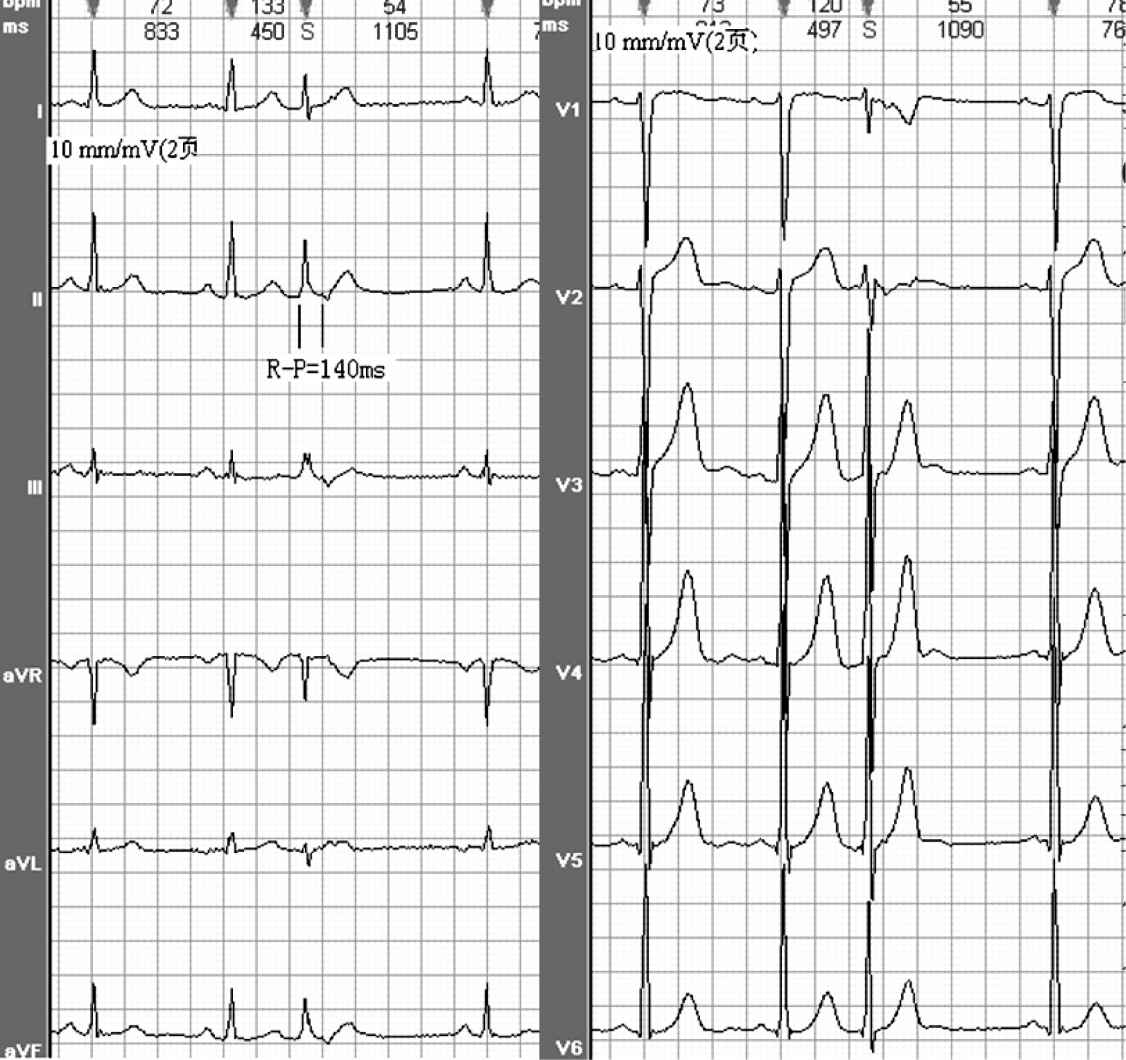
\includegraphics[
    height=.4\textheight,
    width=\textwidth,
    keepaspectratio]{./images/Image00057.jpg}
 \captionsetup{justification=centering}
 \caption{房室交界性期前收缩}
 \label{fig2-2-12}
  \end{figure} 

【治疗方案】 以病因治疗和去除诱因为主,通常无需应用抗心律失常药物。

{(三)加速性交界性心动过速}
 由于激动起源异常或交界区内传导异常而引起的非持续性心动过速,通常频率70\textasciitilde{}130次/分,QRS呈室上性,律齐,可出现房室分离,也可有逆行P波;当窦性心率和加速性交界性心动过速的心率相近时,可出现窦性心律和交界性心律交替控制心室。本病多为病理性,常见原因包括,急性心肌梗死、洋地黄过量、电解质紊乱、应用异丙肾上腺素类药物、风湿病等。

【治疗方案】 治疗原发病。对加速性交界性心动过速无需特殊处理。

{(四)阵发性房室交界性心动过速}
 主要包括房室结折返性心动过速(AVNRT)和房室折返性心动过速(AVRT)。心电图特征如图\ref{fig2-2-13}所示。

\begin{figure}[!htbp]
 \centering
 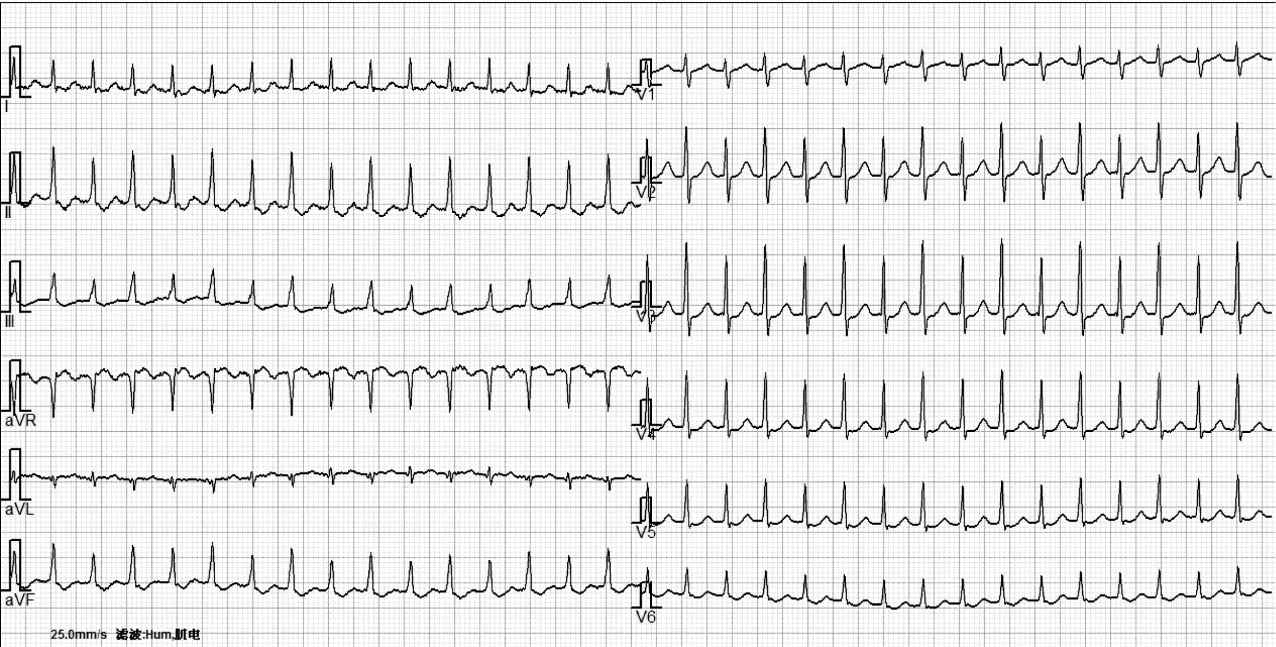
\includegraphics[
    height=.3\textheight,
    width=\textwidth,
    keepaspectratio]{./images/Image00058.jpg}
 \captionsetup{justification=centering}
 \caption{阵发性房室交界性心动过速}
 \label{fig2-2-13}
  \end{figure} 

1.
由房室结折返引起的室上速 称为AVNRT,在房室结可能存在纵向分离的两条通道,即慢通道(α)和快通道(β),慢通道不应期短,传导速度慢;快通道不应期长,传导速度快。窦性心律时,冲动从快通道、慢通道同时下传,快通道下传的冲动先到达希氏束;而慢通道下传的冲动到达希氏束时,不表现出来。当某一房性期前收缩发生时,如此时快通道处于窦性冲动不应期中,慢通道由于其不应期短,已脱离不应期,该房性期前收缩冲动从慢通道下传,当达到希氏束时,如快通道也已脱离不应期,则冲动除继续下传外,也可通过快通道逆传到达心房,如此时慢通道仍未脱离不应期,则可能形成一心房回复波;如慢通道脱离不应期,冲动又可经慢通道下传,在房室结形成冲动传导的折返环,引起室上性心动过速。此类室上性心动过速有两种类型,一为慢快型,即慢通道下传,而快通道逆传,大多数属于此类型;二为快慢型,即快通道下传,慢通道逆传,相对少见。

心电图特点为:室上性QRS波,频率多在150\textasciitilde{}220次/分,心律齐;可由房性或室性期前收缩诱发;逆行性P可落在QRS波中,或在QRS起始部位,或落在QRS波终末部,与窦性QRS波比较,其QRS波起始或终末部与窦性有所不同,还可落在QRS波后面,此时的RP间期小于50\%的PR间期;少数情况下,经慢通道下传,快通道逆传,则逆行的P波落在ST段或在T波上,RP间期稍长,RP/PR\textgreater{}0.75,可有RP\textgreater{}PR。

2.
由房室间旁道折返引起的心动过速 称为AVRT,其心电图表现为:QRS频率150\textasciitilde{}250次/分,节律规则;QRS波群形态与时限正常时,为旁道逆传型AVRT,QRS波群宽大畸形和右δ波时,常为旁道前传型AVRT;可见逆行P波,RP间期一般大于110\textasciitilde{}150毫秒。

【治疗程序】

1. 窄QRS波心动过速鉴别诊断 图\ref{fig2-2-14}所示。

\begin{figure}[!htbp]
 \centering
 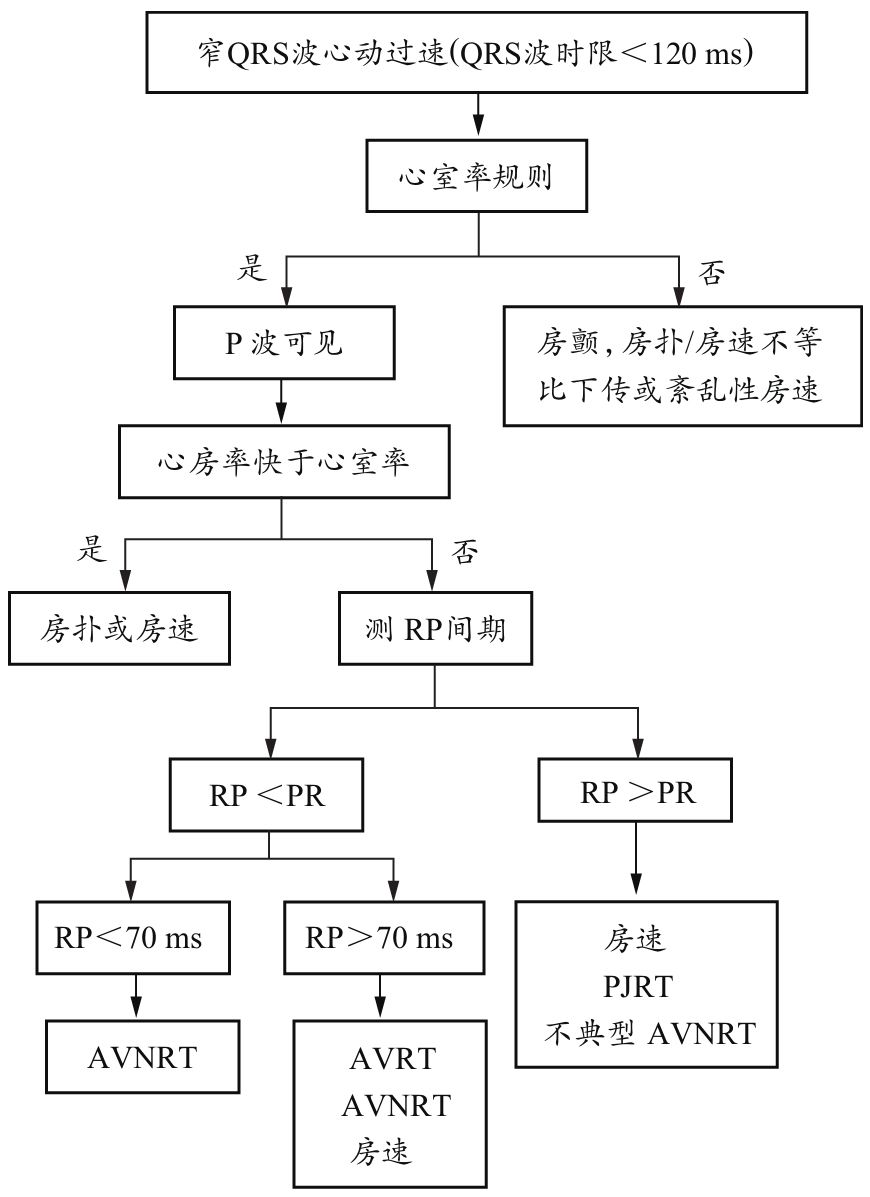
\includegraphics{./images/Image00059.jpg}
 \captionsetup{justification=centering}
 \caption{窄QRS波心动过速的鉴别诊断}
 \label{fig2-2-14}
  \end{figure} 

2. 阵发性室上性心动过速处理流程 图\ref{fig2-2-15}所示。

\begin{figure}[!htbp]
 \centering
 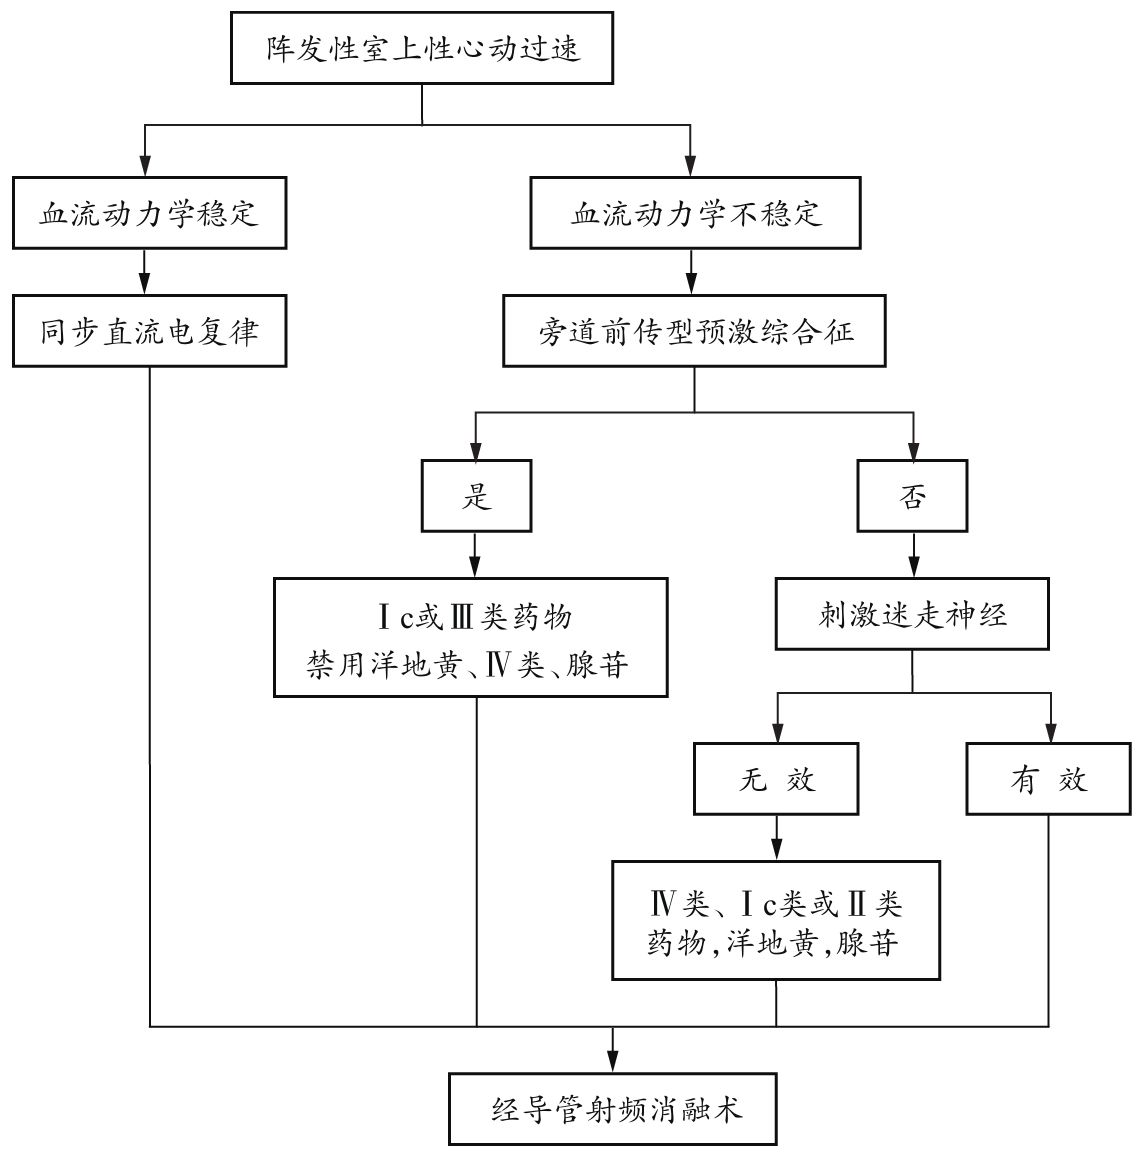
\includegraphics{./images/Image00060.jpg}
 \captionsetup{justification=centering}
 \caption{阵发性室上性心动过速处理流程}
 \label{fig2-2-15}
  \end{figure} 

【治疗方案】

1. AVNRT和旁路逆传型AVRT

(1)复律治疗:发作时应取卧位、吸氧。先行刺激迷走神经法,如刺激呕吐、单侧颈动脉窦按摩等,多可终止室上性心动过速。

上述方法不能终止发作时,可根据情况选用药物治疗或经静脉置入起搏导管,行心腔内刺激以终止室上性心动过速发作,也可通过食道调搏、电复律治疗。药物可选用ATP、普罗帕酮、莫雷西嗪、维拉帕米、毛花苷C、胺碘酮等静脉给药治疗。有血流动力学改变、胸痛者、病情紧急者,可选用同步电复律治疗,神志清醒患者电复律前应静脉缓慢注射地西泮10\textasciitilde{}20mg,当患者处于嗜睡状态,给予50\textasciitilde{}150J能量进行复律。

(2)预防发作:如发作频繁,可用药物有普罗帕酮、莫雷西嗪、维拉帕米、洋地黄类、胺碘酮、丙吡胺等预防发作。

(3)射频消融(RFCA)术:可用于根治。

2.
旁路前传型AVRT 治疗方案基本同前,应避免刺激迷走神经,或延长房室结不应期药物如洋地黄、维拉帕米等,因其使旁道不应期缩短,增加心房扑动、心房颤动时的室性心率,诱发致命性心律失常。常选用普罗帕酮、索他洛尔、普鲁卡因胺或胺碘酮等治疗;症状严重者应立即行电复律治疗。RFCA可根治之。

【疗效观察与随访】 疗效判断以心电图表现为标准。显效:在规定时间内转复为窦性心律,且观察期内无不良反应;有效:在规定时间内转复为窦性心律,但观察期内有不良反应;无效:未能转复为窦性心律。

随访:心律、心率恢复正常后,仍应不定期地注意对心律、心率的监测,必要时复查心电图。

【治疗经验与解析】 单剂口服药物治疗适用于AVNRT发作不频繁,但发作后持续时间长、血流动力学状态稳定、不易自发终止、刺激迷走神经不敏感的患者。心功能不全、窦性心动过缓或有预激的患者不宜接受该治疗方法。无心脏结构和功能异常的青少年和成年人单剂口服氟卡尼(3mg/kg)或普罗帕酮(6mg/kg)可使部分AVNRT终止或频率明显减慢。

{(五)预激综合征}
 预激综合征指室上性激动在下传过程中,通过房室传到副束(旁道),预先激动一部分心室肌的一种综合征。常见旁道有Kent束(连接心房肌与心室肌)、James束(连接心房肌与希氏束)和Mahaim束(连接房室结下部与室间隔)。该综合征多见于无其他心脏异常者,少数可伴发其他器质性心脏病。除病因相关表现外,单纯心室肌预激很少引起临床不适,但可伴发多种心律失常,以AVRT最为常见,亦可伴发房早、室早、房扑和房颤等,少数伴房颤或房扑时可伴发室颤。心电图特征为:PR间期缩短,出现δ波,继发性ST-T改变等。

【治疗方案】 单纯预激综合征以往认为无需治疗,近年认为可能影响心肌重构,也可考虑RFCA。伴发心律失常者,可根据心律失常类型进行相应治疗。RFCA可根治。

【疗效观察与随访】 疗效判断以心电图表现为标准。显效:在规定时间内转复为窦性心律,且观察期内无不良反应;有效:在规定时间内转复为窦性心律,但观察期内有不良反应;无效:未能转复为窦性心律。

随访:复律后仍应注意监测心律、心率的变化,必要时复查心电图,有条件者应寻找其病因,并消除病因。

【治疗经验与解析】

1.
抗心律失常药物可用于治疗旁路参与的心律失常,但近年已逐渐被导管射频消融所替代。

2.
对于心动过速发作不频繁的患者,可采用单剂口服药物治疗,在心动过速发作时服用。该法适用于心电图上无δ波的患者。心动过速发作不频繁、血流动力学稳定的患者,可口服地尔硫䓬
(120mg)加普萘洛尔(80mg),约有80\%的患者在2小时内心动过速可以终止。另外也应用过单剂氟卡尼终止室上速急性发作,但疗效明显低于地尔硫䓬
和普萘洛尔合用。

\subsection{室性心律失常}

{(一)室性逸搏}
 室性逸搏是基本心搏延迟或阻滞,心室潜在起搏点被动发出冲动产生心搏。室性逸搏的心电图表现为长间歇后出现宽大畸形的QRS波。QRS时限一般\textgreater{}0.12秒,少数发生于束支近端的室性逸搏,其QRS波畸形可不明显。逸搏周期在1.5秒以上,很少有逆传P'波。

【治疗方案】 室性逸搏本身无需治疗。

{(二)室性期前收缩}
 室性期前收缩简称室早,是一种最常见的心律失常。室早可见于健康人(尤其健康年轻人),也可由冠心病、瓣膜性心脏病、高血压病、心肌病、甲状腺功能亢进等疾患、药物不良反应或中毒和电解质紊乱引起。

临床表现除病因相关表现外,偶发室早常无明显症状。频发室早可引起心悸、咽部不适或室早后心搏增强感等,原有左心功能不全者可诱发眩晕、黑矇或晕厥,但个体差异较大。

QRS波群提早出现,其形态异常,时限大多\textgreater{}0.12秒,T波与QRS波主波方向相反,ST随T波移位,其前无P波。发生于束支近端处的室性期前收缩,QRS波可不增宽。室性期前收缩后大多有完全代偿间歇。基本心律较慢时,室性期前收缩可插入于两次窦性心搏之间,形成插入型室性期前收缩。偶见室性期前收缩逆传至心房的逆行P'波,常出现于室性期前收缩ST段上(图\ref{fig2-2-16})。

\begin{figure}[!htbp]
 \centering
 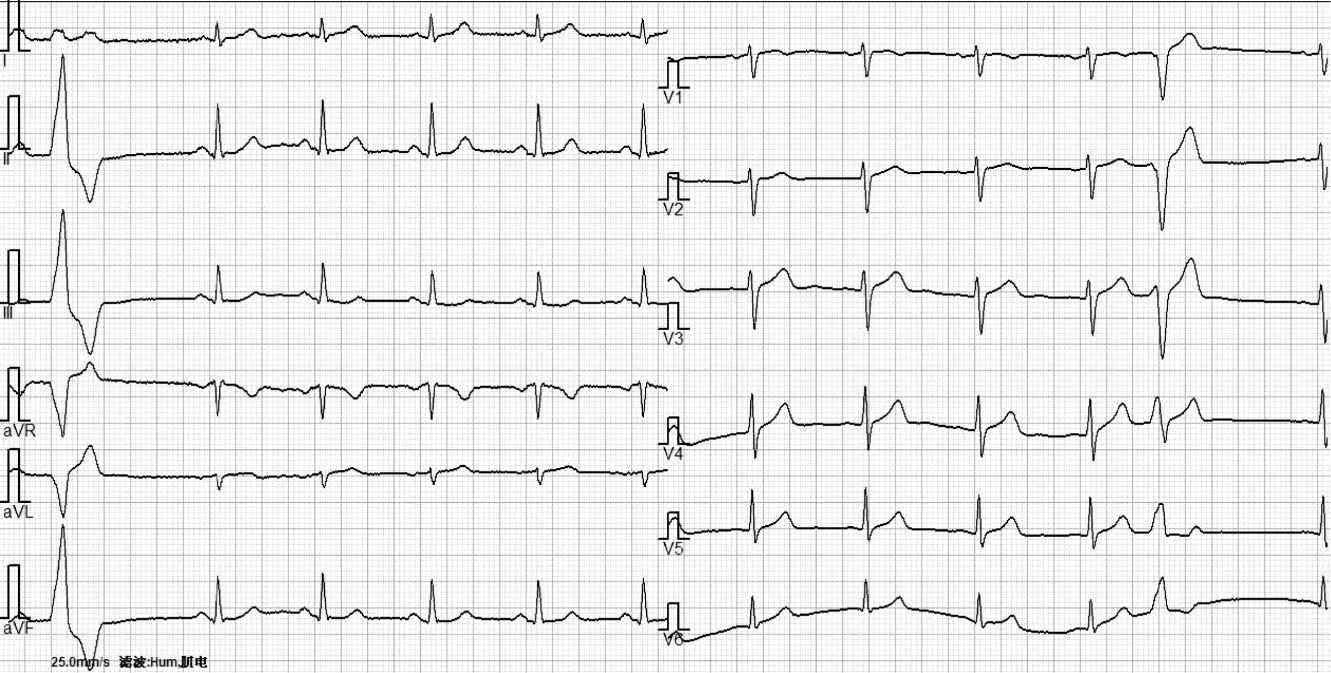
\includegraphics[
    height=.3\textheight,
    width=\textwidth,
    keepaspectratio]{./images/Image00061.jpg}
 \captionsetup{justification=centering}
 \caption{室性期前收缩}
 \label{fig2-2-16}
  \end{figure} 

【治疗程序】 如图\ref{fig2-2-17}所示。

\begin{figure}[!htbp]
 \centering
 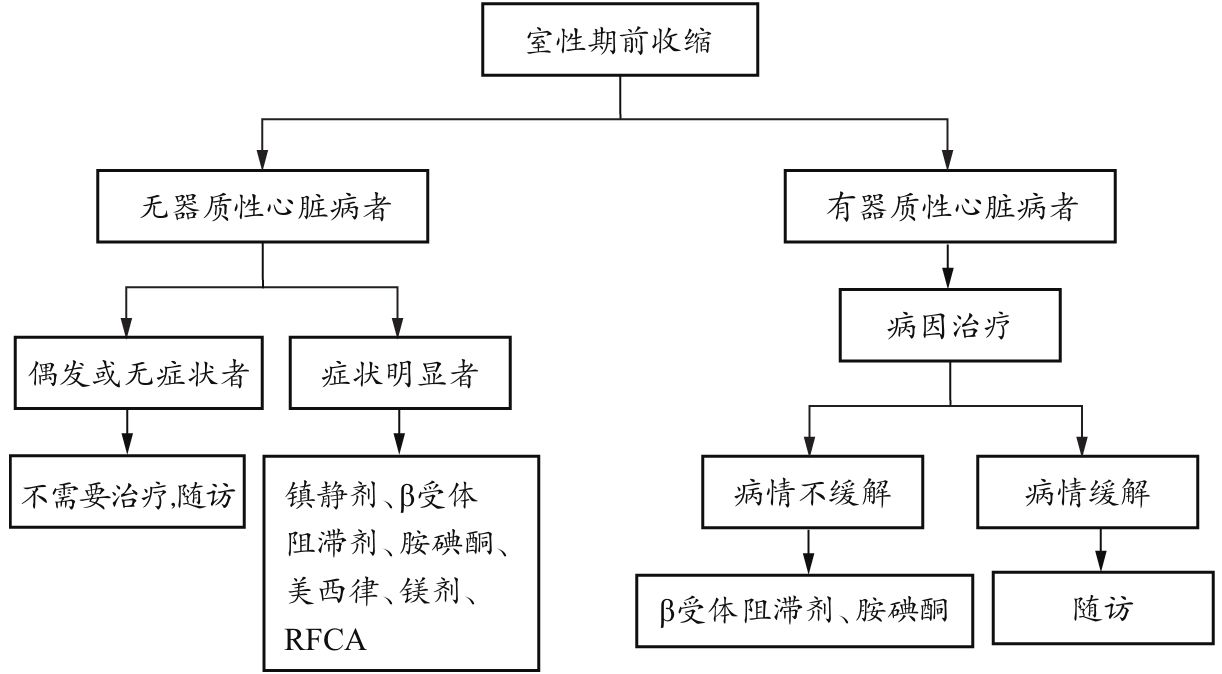
\includegraphics{./images/Image00062.jpg}
 \captionsetup{justification=centering}
 \caption{室性期前收缩的治疗程序}
 \label{fig2-2-17}
  \end{figure} 

【治疗方案】

1.
无器质性心脏病患者 偶发或无症状者无需治疗,症状明显者可应用镇静剂、β受体阻滞剂、胺碘酮及美西律等,适当补充镁剂;起源于左室的室性期前收缩可尝试维拉帕米治疗。部分室性期前收缩,尤其起源于右心室流出道者,可尝试射频消融治疗。

2.
有器质性心脏病患者 首先治疗原发病,对复杂型室早酌情使用抗心律失常药物。

【疗效观察与随访】 观察患者的症状、体征以及心电图转归。

【治疗经验与解析】 β受体阻滞剂是治疗本病及预防恶性心律失常相对安全有效的药物,其他抗心律失常药对于恶性心律失常预防的证据不多,不宜作为一线推荐。

{(三)室性心动过速}
 室性心动过速(VT,简称室速)是指起源于心室、自发、连续3个或以上、频率大于100次/分的期前收缩组成的心律。

VT的分类目前无统一的国际标准。根据VT持续时间、对血流动力学影响、VT形态、引起病因等进行分类。根据室速持续时间可分为:①持续性VT(SuVT),指VT发作持续时间达到或超过30s,或未达30s、已出现严重的血流动力学改变。②非持续性VT(NSuVT),指VT发作持续的时限未达到30s,在30s内能自行终止者。根据VT发作QRS形态,可分为单形性VT、多形性VT。根据持续时间和形态可分为单形性持续性VT、单形性非持续性VT、多形性持续性VT和多形性非持续性VT。根据病因VT可分为缺血性VT、药物性VT、再灌注性VT、右室发育不良性VT等。

VT的原因很多,常见的有冠心病、扩张型心肌病、肥厚型心肌病、心瓣膜病、急性心肌炎、二尖瓣脱垂、抗心律失常药物、抗精神病药(如三环类)、离子通道病(如长QT综合征、Brugada综合征以及儿茶酚胺敏感性室速等)。VT的诱发因素有感染、电解质紊乱特别是低钾血症、运动、情绪波动、咖啡、吸烟、嗜酒等。

临床电生理研究表明,大部分室速是由折返机制引起,自律性增高是部分室速的发病机制,这类室速通常不能被电生理程序刺激终止。

临床表现与室速的持续时间、心率、患者年龄、基础疾病、心功能密切相关,患者症状一般较室上速严重。临床症状包括心悸、胸闷、气急、胸痛、头晕、黑矇、晕厥、休克,甚至阿-斯综合征发作。体检发现患者精神紧张、神情淡漠、甚至昏迷;有些患者脉搏不易扪及,脉搏短绌、交替脉,有些血压下降或测不出等,如有房室分离,颈静脉搏动可见大炮A波、第一心音强弱不等、偶可闻及大炮音,心律通常均齐,也有心律不齐者,心率一般在130\textasciitilde{}200次/分,有时肺部可闻及哮鸣、湿性啰音等表现。部分患者无明显不适症状,或仅有心悸,体格检查除心率较快外无特殊发现,见于无明显基础疾病发作时心室率相对较慢者。

【治疗程序】

1. 心室率规则的血流动力学稳定的心动过速的处理程序 如图\ref{fig2-2-18}。

\begin{figure}[!htbp]
 \centering
 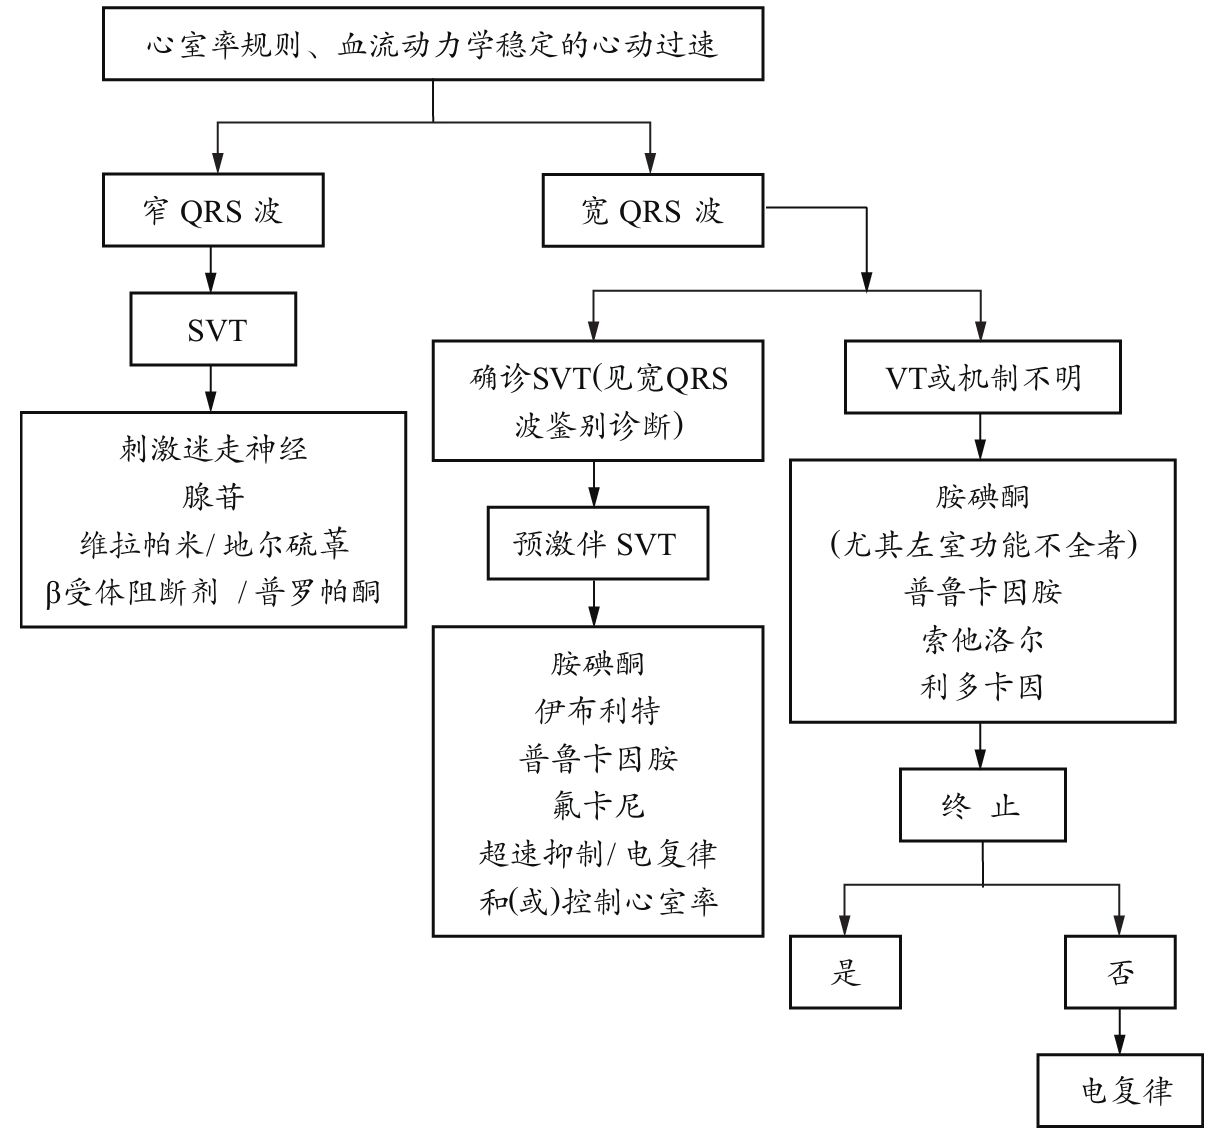
\includegraphics{./images/Image00063.jpg}
 \captionsetup{justification=centering}
 \caption{心室率规则的血流动力学稳定的心动过速的处理程序}
 \label{fig2-2-18}
  \end{figure} 

【治疗方案】

1.
终止发作 持续性室速的治疗根据其对血流动力学影响而不同。患者有显著血流动力学障碍,如有血压下降、神志模糊、休克表现者,立即予以同步直流电复律;可在麻醉下行同步电复律,复律能量以100\textasciitilde{}250J为宜,同时应寻找诱发因素,纠正电解质与酸碱平衡紊乱、停用诱发室速药物等。无明显血流动力学改变者,可静脉给予药物治疗,如利多卡因、胺碘酮、普罗帕酮、硫酸镁等。心室率规则的血流动力学稳定的心动过速的药物治疗,见表\ref{tab2-2-1}。

\begin{longtable}[]{@{}lllll@{}}
    \caption{心室率规则且血流动力学稳定的心动过速的治疗}
    \label{tab2-2-1}\\
\toprule
ECG & 处理 & & 推荐级别 & 证据级别\tabularnewline
\midrule
\endfirsthead
\caption[]{心室率规则且血流动力学稳定的心动过速的治疗}\\
\toprule
ECG & 处理 & & 推荐级别 & 证据级别\tabularnewline
\midrule
\endhead
\bottomrule
\endfoot
窄QRS波心动过速(SVT) &
\vtop{\hbox{\strut 刺激迷走}\hbox{\strut 腺苷}\hbox{\strut 维拉帕米,地尔硫䓬}\hbox{\strut β受体阻滞剂}\hbox{\strut 胺碘酮}\hbox{\strut 地高辛}}
& &
\vtop{\hbox{\strut Ⅰ}\hbox{\strut Ⅰ}\hbox{\strut Ⅰ}\hbox{\strut Ⅰb}\hbox{\strut Ⅰb}\hbox{\strut Ⅰb}}
&
\vtop{\hbox{\strut B}\hbox{\strut A}\hbox{\strut A}\hbox{\strut C}\hbox{\strut C}\hbox{\strut C}}\tabularnewline
宽QRS波心动过速 & & & &\tabularnewline
  ·SVT+BBB & & 同SVT & &\tabularnewline
  ·预激综合征SVT+AF &
\vtop{\hbox{\strut 氟卡尼}\hbox{\strut 伊布利特}\hbox{\strut 普鲁卡因胺}\hbox{\strut 直流电复律}\hbox{\strut 普鲁卡因胺}\hbox{\strut 索他洛尔}\hbox{\strut 胺碘酮}}
& &
\vtop{\hbox{\strut Ⅰ}\hbox{\strut Ⅰ}\hbox{\strut Ⅰ}\hbox{\strut Ⅰ}\hbox{\strut Ⅰ}\hbox{\strut Ⅰ}\hbox{\strut Ⅰ}}
&
\vtop{\hbox{\strut B}\hbox{\strut B}\hbox{\strut B}\hbox{\strut C}\hbox{\strut B}\hbox{\strut B}\hbox{\strut B}}\tabularnewline
  ·未知类型的宽QRS波心动过速 &
\vtop{\hbox{\strut 直流电复律}\hbox{\strut 利多卡因}\hbox{\strut 腺苷}\hbox{\strut β受体阻滞剂}\hbox{\strut 维拉帕米}}
& &
\vtop{\hbox{\strut Ⅰ}\hbox{\strut Ⅰb}\hbox{\strut Ⅰb}\hbox{\strut Ⅱ}\hbox{\strut Ⅱ}}
&
\vtop{\hbox{\strut B}\hbox{\strut B}\hbox{\strut C}\hbox{\strut C}\hbox{\strut B}}\tabularnewline
未知类型的宽QRS波心动过速伴左室功能障碍 &
\vtop{\hbox{\strut 胺碘酮}\hbox{\strut 直流电复律,利多卡因}} & &
\vtop{\hbox{\strut Ⅰ}\hbox{\strut Ⅰ}} &
\vtop{\hbox{\strut B}\hbox{\strut B}}\tabularnewline
\end{longtable}

2.
预防发作 VT患者多有器质性心脏病。预防VT的药物包括硫酸镁、美西律、利多卡因、普罗帕酮、普鲁卡因胺、胺碘酮、丙吡胺、β受体阻滞剂、奎尼丁等。心肌梗死后患者避免使用普罗帕酮、氟卡胺、英卡胺或莫雷西嗪治疗。发作频繁者应建议住院治疗。

3.
外科治疗 顽固性室速患者,明确由心肌梗死后的室壁瘤引起,可行外科手术切除。该法并未显著改善患者预后,其获益受到质疑。无室壁瘤患者,可行心内膜标测定位,并行直视下心内膜病灶切除术,可望奏效。如果室速与瓣膜疾病有关,行瓣膜置换术可能有效;特发性LQTS患者,颈胸交感神经结切除术有一定疗效;肥厚型梗阻性心肌病患者,手术切除其室间隔肥厚部位心肌对预防猝死有效。

4.
埋植型自动心律转复除颤器(ICD) 已成为有危及生命的室性心律失常首选治疗手段,可显著降低室速患者死亡危险,但价格昂贵,且放电时患者十分痛苦,需严格掌握ICD植入的适应证。

5.
导管消融治疗 对冠心病、心肌梗死后的室速疗效差,对无器质性心脏病的分支性室速,或单形性室速疗效较好。

【疗效观察与随访】

1. 观察治疗前后患者症状、体征以及心电图、动态心电图等转归。

2. 室性心律失常与猝死无创预测指标 见表\ref{tab2-2-2}。


\begin{longtable}[]{lp{8cm}}
    \caption{室性心律失常与猝死无创预测指标}
    \label{tab2-2-2}\\
\toprule
方 式 & 结 论\tabularnewline
\midrule
\endfirsthead
\caption[]{室性心律失常与猝死无创预测指标}\\
\toprule
方 式 & 结 论\tabularnewline
\midrule
\endhead
\bottomrule
\endfoot
左室射血分数(LVEF) &
LVEF作为猝死(SCD)的预测因子已经广为人知。低LVEF患者是SCD的高危人群,需要进一步干预,然而LVEF预测SCD仍然有其局限性,大多数发生SCD的患者LVEF并非明显降低\tabularnewline
心电图(ECG) &\tabularnewline
 ·QRS波时限 &
大多数回顾性研究显示QRS波增宽是SCD的危险因素。临床有效性尚未验证\tabularnewline
 ·信号平均心电图(SAECG) &
由于主要基于前瞻性研究,SAECG异常很可能是SCD的危险因素。临床有效性已经开始验证,尚未得出结论\tabularnewline
 ·短程心率变异性(HRV) &
短程HRV异常是否能预测SCD尚缺乏数据说明。临床有效性尚未验证\tabularnewline
动态心电图(Holter) &\tabularnewline
 ·室性早搏和非持续性室速(NSVT) &
动态心电图记录的室性心律失常(VPBs,NSVT)是SCD重要预测因素。在某些人群中,NSVT被作为预测心律失常性SCD而进一步干预治疗,但灵敏度可能有限\tabularnewline
 ·长程心率变异性(HRV) &
HRV减低是死亡率的一个重要危险因素,并非SCD特有。临床有效性已经开始验证,尚未得出结论\tabularnewline
 ·心率震荡 &
最近数据表明心率震荡可能是SCD的危险因素。临床有效性尚未验证\tabularnewline
运动试验/功能状态 &\tabularnewline
 ·运动能力和纽约心功能(NYHA)分级 &
心功能的严重程度是SCD的危险因子,在预测进行性泵衰竭方面更重要。临床有效性尚未验证\tabularnewline
 ·心率恢复和恢复期室性早搏 &
心率恢复和恢复期室性早搏是否能预测SCD尚缺乏证据。临床有效性尚未验证\tabularnewline
 ·T波电交替(TWA) &
部分前瞻性研究支持TWA异常作为SCD危险因子。临床有效性正在评估,但结论尚不一致\tabularnewline
\end{longtable}

【治疗经验与解析】

1.
对于室性心律失常患者,应先评估患者发生心源性猝死风险。评估方式多样,常用手段如表\ref{tab2-2-2}“室性心律失常与猝死无创预测指标”所示,若患者属于猝死高危,则须评估ICD植入适应证。

2.
循证医学表明,除β受体阻滞剂外,其他抗心律失常药物无法改善器质性心脏病患者的预后,因此器质性心脏病合并的室速以病因治疗为主,不应过分强调应用抗心律失常药物减少心律失常的作用。

\subsection{心脏传导阻滞}

心脏传导异常是由解剖或功能失常造成的持久或暂时性冲动传导异常。其主要表现在传导阻滞,即传导时间延长,部分或全部传导中断。传导阻滞可分为三度:一度传导阻滞表现为传导时间延长,但无传导中断。二度传导阻滞有莫氏Ⅰ型和莫氏Ⅱ型两种形式,莫氏Ⅰ型的特征为传导时间逐渐延长直至一次传导中断,莫氏Ⅱ型的特征为在传导中断前后无传导时间改变。三度传导阻滞指所有冲动都不能被传导,又称完全性传导阻滞。

心脏传导阻滞根据其阻滞部位,可分为窦房传导阻滞、心房内传导阻滞、房室传导阻滞和室内传导阻滞。

{(一)窦房传导阻滞}  见窦性心律失常章节。

{(二)心房内传导阻滞}
 心房内传导阻滞以P波增宽为心电图表现,P波时限超过0.12s,波峰有切迹见于各种病因引起的心房扩大和心房肌梗死。

【治疗方案】 本病一般不需要药物治疗。

{(三)房室传导阻滞}
 心房激动向心室传导延迟或不能完全传导至心室称为房室传导阻滞(AVB)。病因包括心肌梗死、心肌炎、退行性变、手术损伤、先天缺损等。

1.
一度房室传导阻滞 心电图(图\ref{fig2-2-19})表现为PR间期的延长,通常成人\textgreater{}200ms,无QRS波的脱落。

\begin{figure}[!htbp]
 \centering
 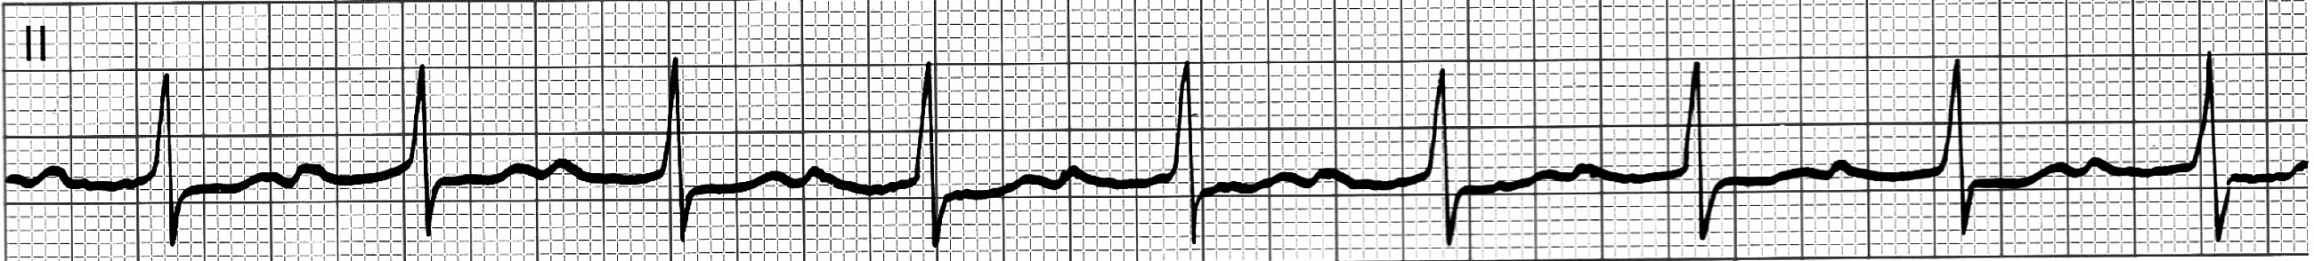
\includegraphics[
    height=.3\textheight,
    width=\textwidth,
    keepaspectratio]{./images/Image00064.jpg}
 \captionsetup{justification=centering}
 \caption{一度房室传导阻滞}
 \label{fig2-2-19}
  \end{figure} 

2.
二度房室传导阻滞 心电图表现为部分P波后无QRS波,P波与QRS波之间可呈规则或不规则比例,QRS波形态正常或称束支阻滞型。

(1)二度Ⅰ型房室传导阻滞:心电图(图\ref{fig2-2-20})表现为PR间期逐渐延长直至P波不能下传,RR间期逐次缩短直至心室脱漏,P波与QRS波比例多不规则。

\begin{figure}[!htbp]
 \centering
 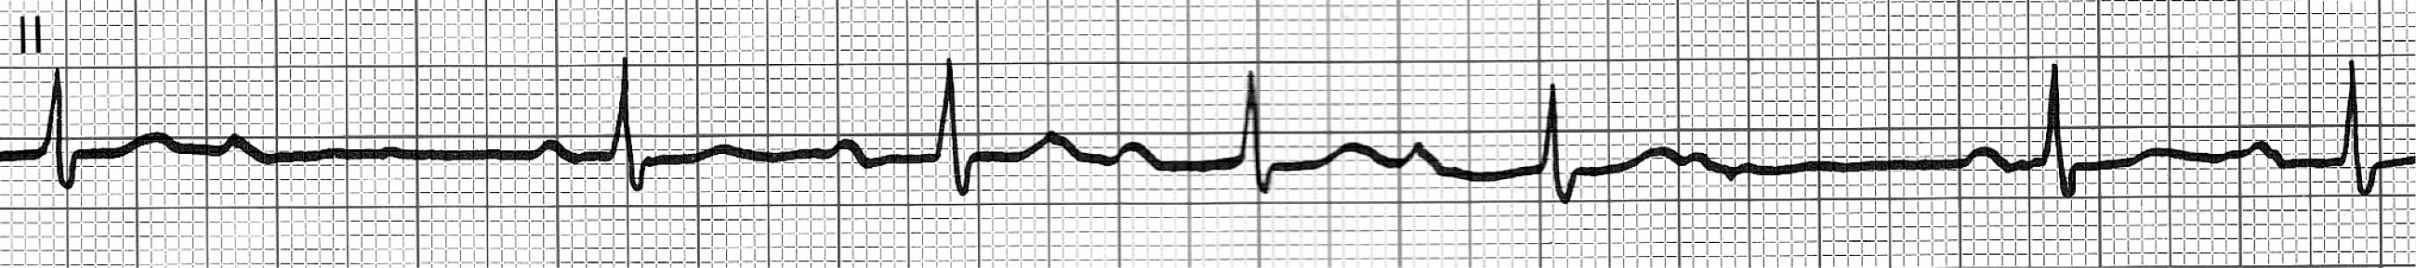
\includegraphics[
    height=.3\textheight,
    width=\textwidth,
    keepaspectratio]{./images/Image00065.jpg}
 \captionsetup{justification=centering}
 \caption{二度Ⅰ型房室传导阻滞}
 \label{fig2-2-20}
  \end{figure} 

(2)二度Ⅱ型房室传导阻滞:心电图(图\ref{fig2-2-21})表现为心室脱漏前PR间期恒定。

\begin{figure}[!htbp]
 \centering
 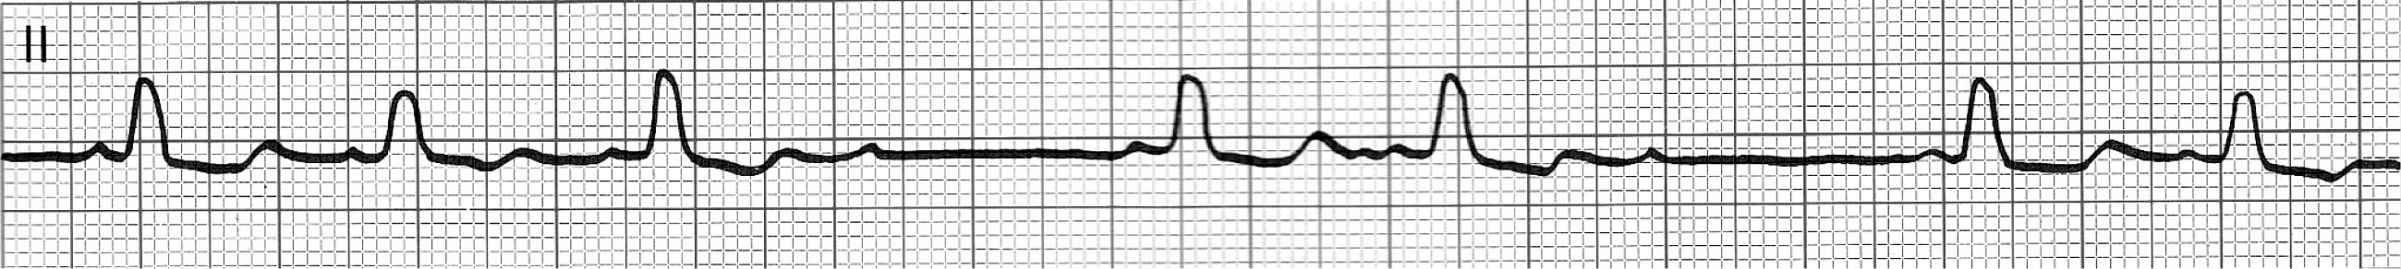
\includegraphics[
    height=.3\textheight,
    width=\textwidth,
    keepaspectratio]{./images/Image00066.jpg}
 \captionsetup{justification=centering}
 \caption{二度Ⅱ型房室传导阻滞}
 \label{fig2-2-21}
  \end{figure} 

3.
三度房室传导阻滞 指所有P波不能下传至心室,心房和心室由各自独立的起搏点控制(图\ref{fig2-2-22})。

\begin{figure}[!htbp]
 \centering
 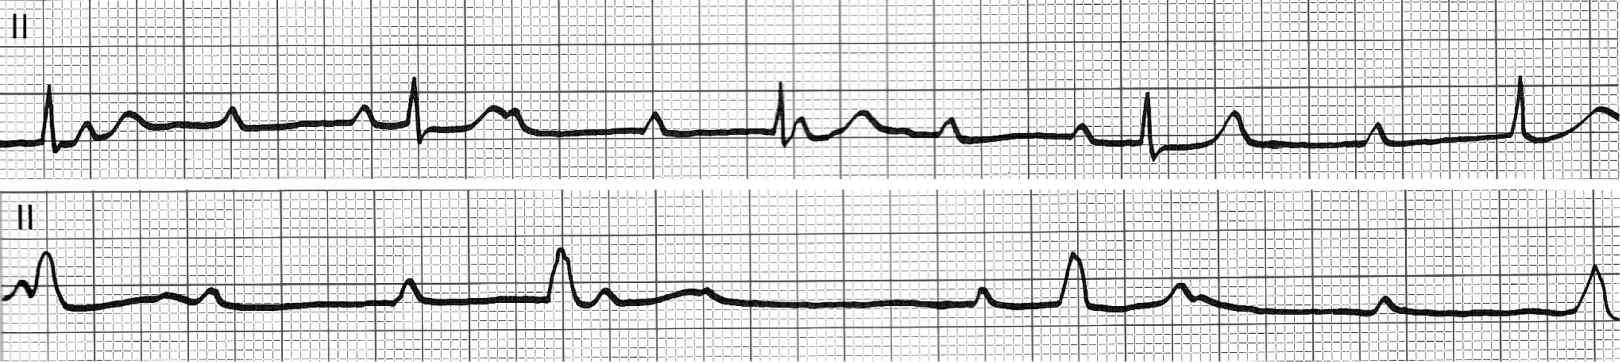
\includegraphics[
    height=.3\textheight,
    width=\textwidth,
    keepaspectratio]{./images/Image00067.jpg}
 \captionsetup{justification=centering}
 \caption{三度房室传导阻滞}
 \label{fig2-2-22}
  \end{figure} 

【治疗程序】 如图\ref{fig2-2-23}所示。

\begin{figure}[!htbp]
 \centering
 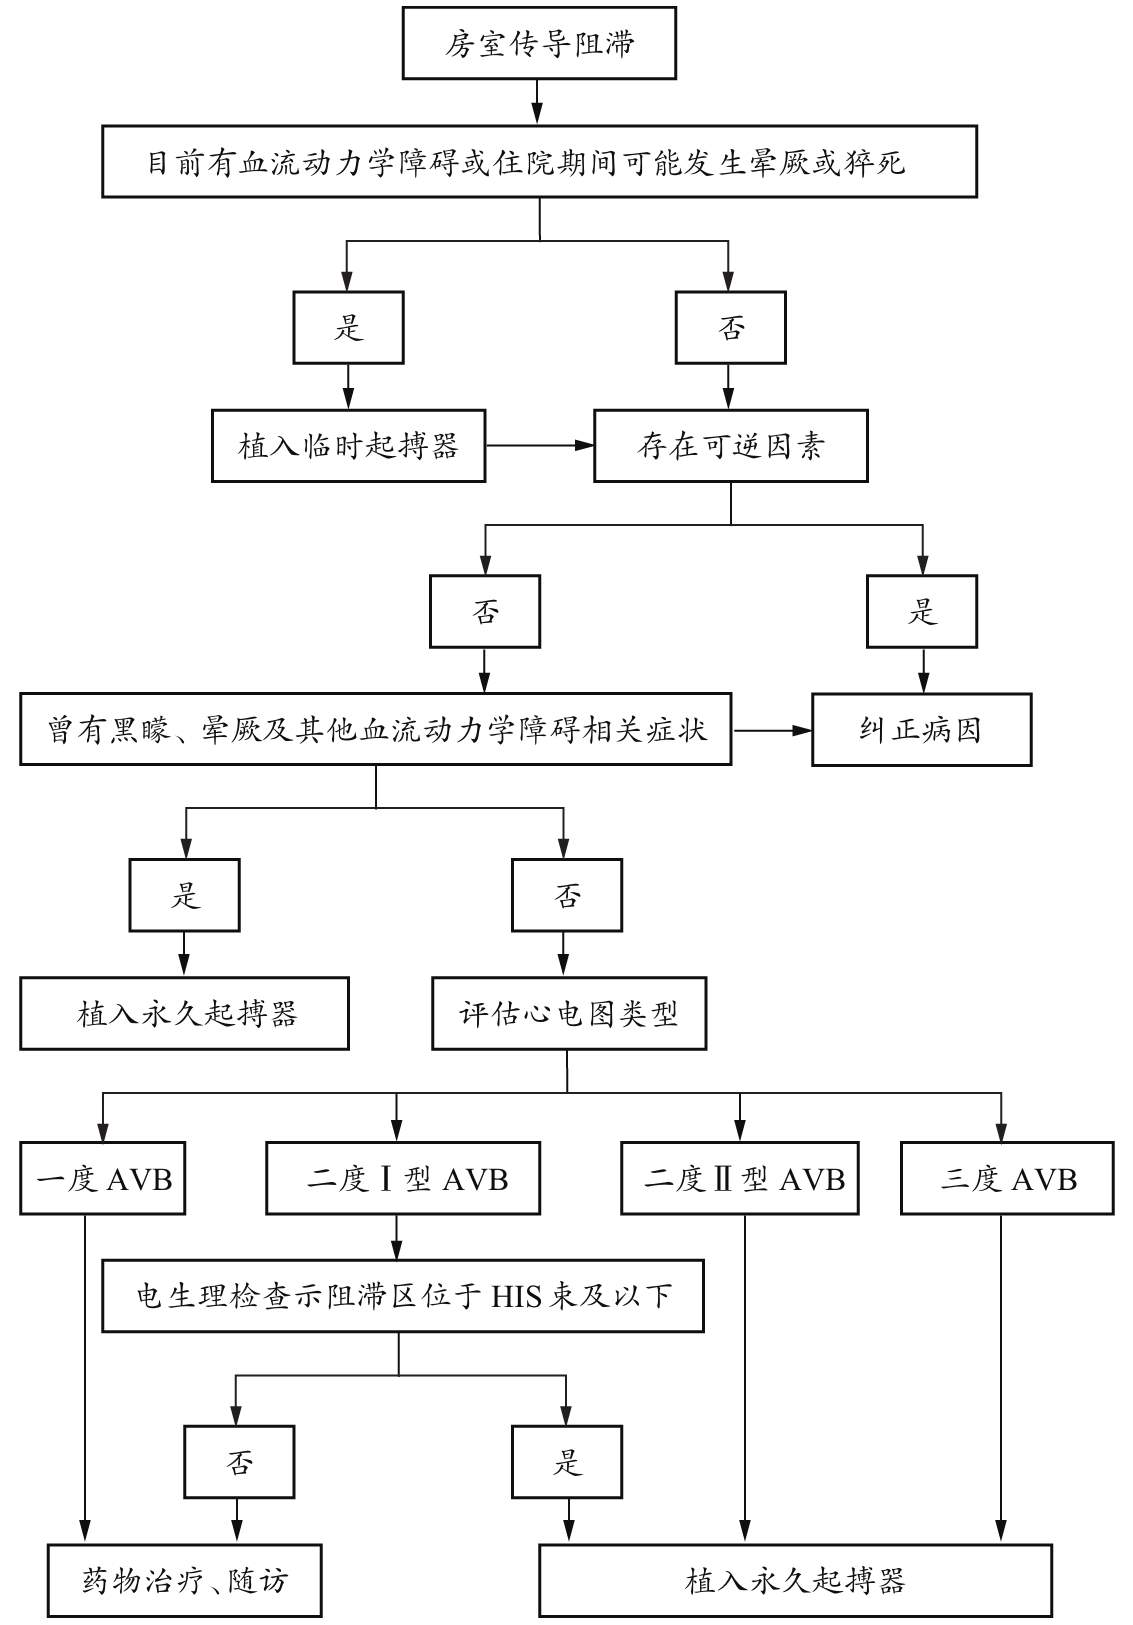
\includegraphics{./images/Image00068.jpg}
 \captionsetup{justification=centering}
 \caption{房室传导阻滞的治疗程序}
 \label{fig2-2-23}
  \end{figure} 

【治疗方案】

1.
病因治疗 包括解除迷走神经过高张力、停用有关药物、纠正电解质紊乱等。各种急性心肌炎、心脏直视术损伤或急性心肌梗死引起的房室传导阻滞可试用糖皮质激素治疗。

2. 药物治疗

(1)拟交感神经药物:常用异丙肾上腺素每4小时含服5\textasciitilde{}10mg,或沙丁胺醇2\textasciitilde{}4mg,每日3\textasciitilde{}4次,或麻黄碱口服,30mg,每日3\textasciitilde{}4次。预防或治疗房室传导阻滞引起的阿-斯综合征发作,宜用0.5mg/dl异丙肾上腺素液连续静脉滴注,控制滴速使心室率维持在60\textasciitilde{}70次/分。

(2)阿托品:每4小时口服0.3mg,适用于房室束分支以上的阻滞,尤其是迷走神经张力过高所致的阻滞,必要时肌内注射或静脉注射,每4\textasciitilde{}6小时0.5\textasciitilde{}1.0mg。

(3)碱性药物:碳酸氢钠或乳酸钠可改善心肌细胞应激性、促进传导系统心肌细胞对拟交感神经药物反应的作用,一般用静脉滴注或推注,尤其适用于高血钾或伴酸中毒时。

3. 人工心脏起搏治疗 参见人工心脏起搏章节。

【疗效观察与随访】 观察治疗前后的症状、体征、心电图以及动态心电图等转归。

【治疗经验与解析】 房室束分支以上阻滞形成的一至二度房室传导阻滞主要针对病因治疗,房室束分支以下阻滞者,不论是否引起房室传导阻滞,均须慎重考虑人工心脏起搏器适应证。

{(四)心室内传导阻滞}

心室内传导阻滞指房室束分支以下的传导障碍。心室内传导阻滞心电图改变包括完全性右束支传导阻滞和完全性左束支传导阻滞。左束支阻滞常提示心室肌弥漫性病变,如冠心病、心肌病或主动脉狭窄等。右束支传导阻滞不一定有广泛心肌损害,常见病因包括风心病、先天性房间隔缺损等,不完全性右束支传导阻滞可见于无心脏病证据的健康人。

1.
完全性右束支传导阻滞(CRBBB) 心电图(图\ref{fig2-2-24})表现为QRS时限0.12秒以上,Ⅰ导联有明显增宽的S波,V1、V2导联有小r波、大R波或R波双峰,V5、V6导联R波窄而高,S波增宽,T波与QRS主波方向相反。

\begin{figure}[!htbp]
 \centering
 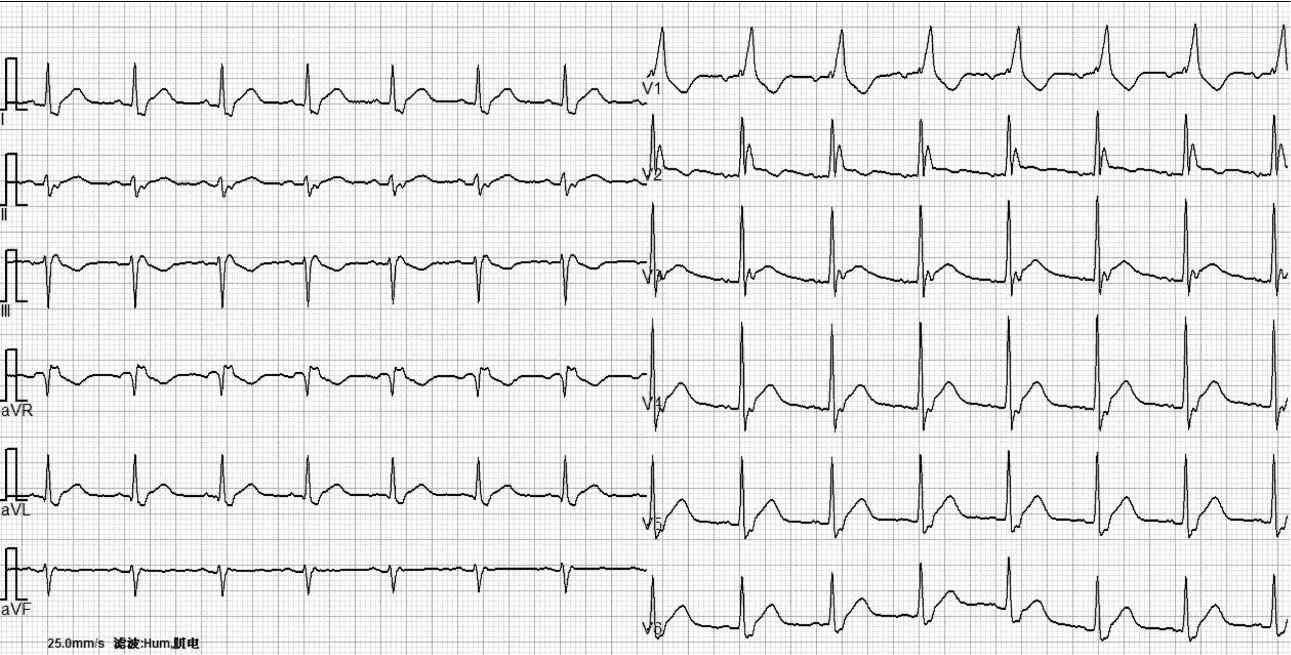
\includegraphics[
    height=.3\textheight,
    width=\textwidth,
    keepaspectratio]{./images/Image00069.jpg}
 \captionsetup{justification=centering}
 \caption{完全性右束支传导阻滞}
 \label{fig2-2-24}
  \end{figure} 

2.
完全性左束支传导阻滞(CLBBB) 心电图(图\ref{fig2-2-25})表现为QRS时限0.12秒以上,Ⅰ导联R波宽大或有切迹,V1、V2导联r波极小,S波宽大,V5、V6导联R波有切迹或呈双重R波,无Q波,T波与QRS主波方向相反。

\begin{figure}[!htbp]
 \centering
 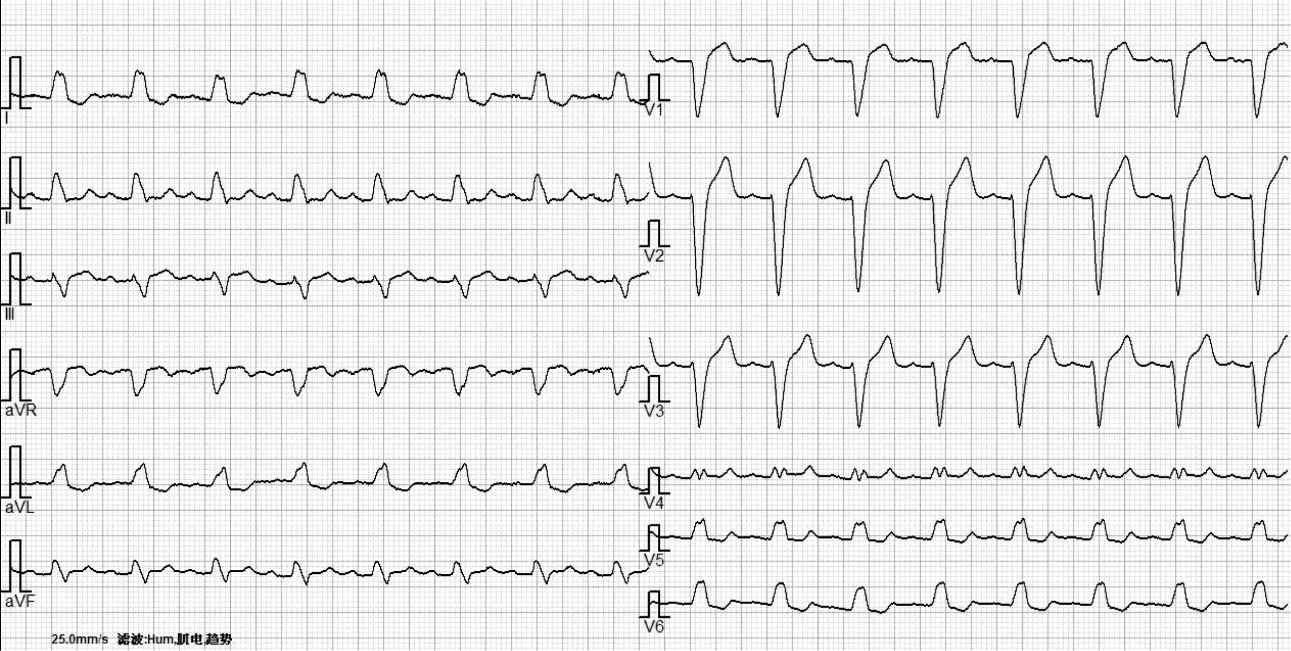
\includegraphics[
    height=.3\textheight,
    width=\textwidth,
    keepaspectratio]{./images/Image00070.jpg}
 \captionsetup{justification=centering}
 \caption{完全性左束支传导阻滞}
 \label{fig2-2-25}
  \end{figure} 

【治疗方案】 一般无需治疗,如果多束支阻滞,出现三度AVB,则行相应治疗。


\section{心脏骤停与心源性猝死}

心脏骤停(suddencardiacarrest,SCA)是指心脏泵血功能的突然终止。多见于器质性心脏病,导致心脏骤停的病理生理学机制常见于快速性心律失常,其次为缓慢性心律失常和心室停搏,较少见于无脉性电活动。心源性猝死(sudden
cardiac
death,SCD)是指由心脏原因引起的突然死亡,通常发生在急性症状发作后1小时内,以意识丧失为特征。心脏骤停和心源性猝死通常是连续的病理生理过程,除少数自行恢复外,不经积极救治的心脏骤停通常是心源性猝死的直接原因。

【治疗程序】 如图\ref{fig2-3-1}所示。

\begin{figure}[!htbp]
 \centering
 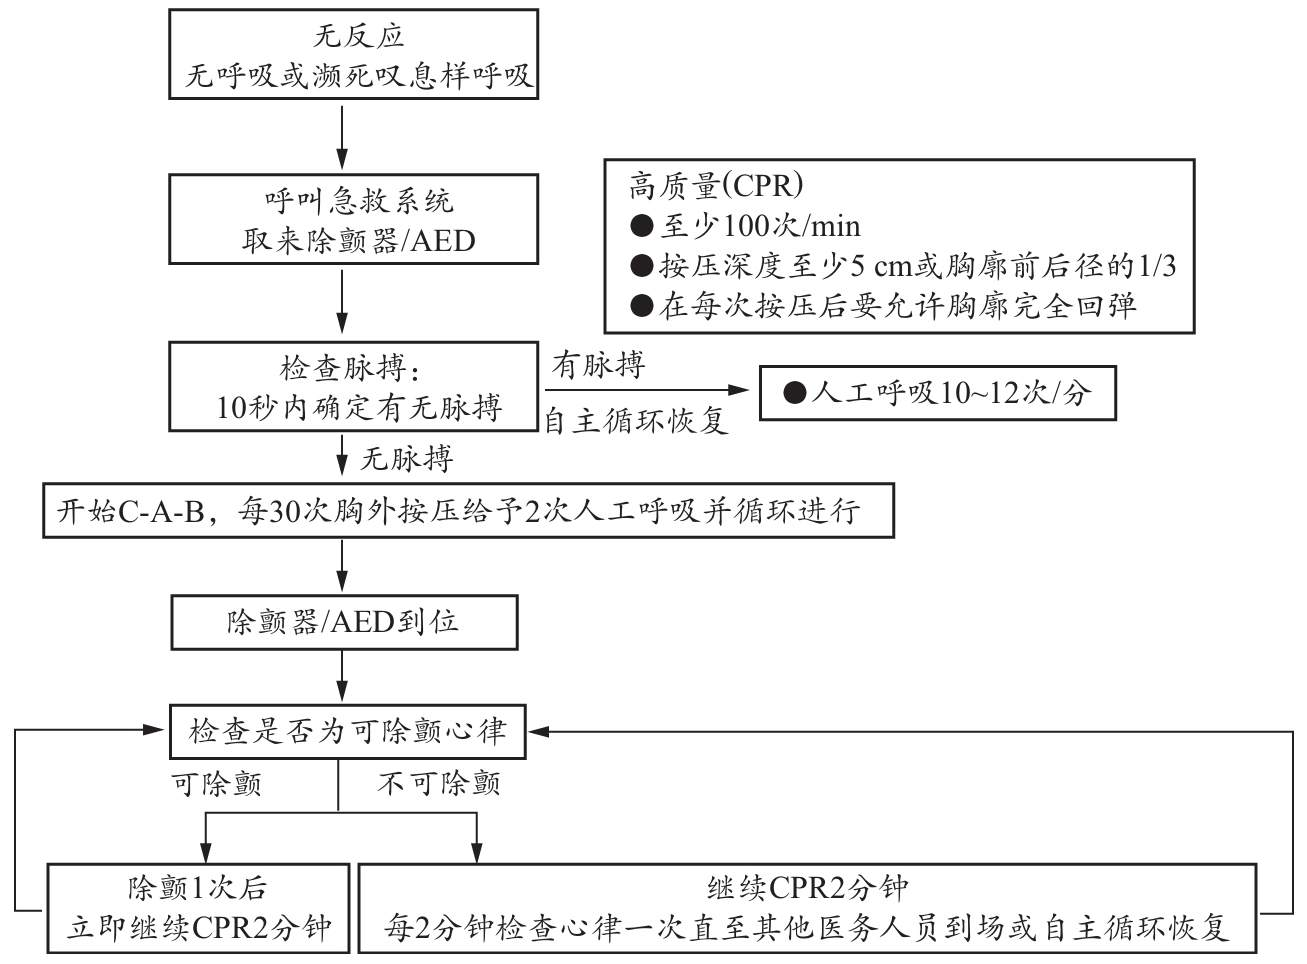
\includegraphics{./images/Image00071.jpg}
 \captionsetup{justification=centering}
 \caption{心脏骤停与心源性猝死的治疗程序}
 \label{fig2-3-1}
  \end{figure} 

【治疗方案】

{(一)基础生命支持}

1.
立即识别和呼叫急救系统 发现患者突然倒地且意识丧失、无呼吸或叹息样呼吸,可判定患者发生SCA,立即启动急救系统,120调度员应指导非专业施救者按步骤施行心肺复苏(CPR)。在启动急救系统后,现场施救者都应立即对该成年患者进行CPR。

2.
脉搏检查 非专业施救人员可以不必检查脉搏直接开始胸外按压。医务人员检查脉搏时间不应超过10秒,如果在10秒内无法明确感觉到脉搏,应开始胸外按压。

3.
尽早开始CPR 成人胸外按压速率每分钟至少100次,且按压深度应为至少5厘米或者胸廓前后径的1/3。在每一次按压后要允许胸廓充分回弹,尽可能避免胸外按压中断,中断时间不应超过10秒。需完成5个循环,约2分钟,再行判断呼吸、心律。未经培训的普通施救者可实施仅做胸外按压的CPR。医务人员应使患者仰头抬颏保持气道通畅,怀疑有颈椎损伤,应使用双下颌上提法而不能拉伸头部。经训练的施救者使用口对口或气囊面罩人工呼吸来供氧及通气。总要求如下:每次通气时间1秒以上;足够的潮气量以使得胸廓抬起;采用按压通气的比率为30∶2。

4.
快速电除颤 现场仅一名施救者时,应先启动急救系统,如有除颤器/AED立即除颤,并立即进行胸外按压。当现场有两名及以上施救者时,一人立即胸外按压,另一人迅速启动急救系统,并取除颤器尽快除颤。在放电后立即继续胸外按压,2分钟后再判断是否除颤成功。

{(二)高级心血管生命支持}

1.
通气与氧供 如患者自主呼吸仍未恢复应尽早行气管插管,院外予面罩或简易球囊维持通气,院内采用呼吸机,通常初始采用容量控制通气模式,潮气量设定为6\textasciitilde{}7ml/kg或500\textasciitilde{}600ml,根据动脉血气结果调整参数。

2. 除颤、复律与起搏治疗

(1)室颤/无脉性室速:抢救人员应立即应用除颤器给予一次电击,能量双相波为200J,单相波为360J。前侧位是首选的电极位置,在不同情况下电极贴选择前-后、前-左肩胛下和前-右肩胛下位均是合理的。电击后立即从胸外按压开始继续进行CPR2分钟,再检查心律,如需要可再次电击。如果电击后室颤终止,但稍后室颤又复发,可按前次能量再次电击。治疗室颤/无脉性室速期间,医务人员必须保证CPR的其他操作如胸外按压与人工通气和电除颤之间的有效协调。当至少1次除颤和2分钟CPR后室颤/无脉性室速仍持续时,可给予肾上腺素或血管加压素。当室颤/无脉性室速对CPR、除颤和血管活性药均无反应时,可给予胺碘酮。如无胺碘酮,可给予利多卡因。

(2)无脉性电活动/心室停搏:抢救人员应立即进行CPR2分钟,再重新检查心律,观察心律有无变化,如无变化继续循环进行上述抢救措施。有应用抢救药品的条件时,应给予肾上腺素或血管加压素,不推荐使用阿托品。

3. 药物治疗 可选择的给药途径包括经外周静脉、骨髓腔、中心静脉和气管。

(1)肾上腺素:主要作用为激动α-肾上腺素能受体提高CPR期间的冠状动脉和脑动脉灌注压。在ACLS期间,在至少2分钟CPR和1次电除颤后,每3\textasciitilde{}5分钟应经静脉或骨髓腔注射1次1mg肾上腺素。递增肾上腺素剂量方法不能提高患者存活率。

(2)血管加压素:与肾上腺素相比在预后上无差异。可经静脉或骨髓腔应用一次血管加压素40U替代第1或第2次剂量的肾上腺素。

(3)胺碘酮:可以用于对CPR、除颤和血管活性药治疗无反应的室颤或无脉性室速,首剂为300mg(或5mg/kg)经静脉或骨髓腔内注射,用20ml的5\%葡萄糖溶液稀释后快速推注,随后电除颤1次,如仍未转复,可于10\textasciitilde{}15分钟后再次应用150mg,如需要可重复6\textasciitilde{}8次。在首个24小时内使用维持剂量,开始6小时内1mg/min,后18小时为0.5mg/min,总量不超过2.0\textasciitilde{}2.2g。

(4)碳酸氢钠和溶栓治疗:对SCA患者,不常规使用碳酸氢钠和溶栓治疗。用适当的有氧通气恢复氧含量、用高质量的胸外按压维持组织灌注和心排出量,然后尽快恢复自主循环,是恢复SCA期间酸碱平衡的主要方法。当代谢性酸中毒是SCA病因等特殊情况下可使用碳酸氢钠。溶栓治疗增加颅内出血风险,但怀疑或确定肺栓塞是SCA的病因时,可考虑经验性溶栓治疗。

(5)其他备选的血管活性药:与肾上腺素相比,其他的血管活性药(去甲肾上腺素等)并不能提高存活率。

{(三)综合的心脏骤停后治疗}

1. 气体交换的最优化 气管插管患者应进行CO{2}
波形图监测。用脉搏血氧饱和度测定仪持续监测患者氧合情况。维持脉搏血氧饱和度在94\%\textasciitilde{}99\%。避免肺或其他脏器发生氧中毒。

2.
心脏节律和血流动力学监测和管理 评估生命体征及监测心律失常复发。在自主循环恢复后、转运及住院期间都要进行连续心电监护直至患者稳定。静脉使用血管活性药物如肾上腺素、多巴胺、去甲肾上腺素等,并逐步调整剂量使收缩压≥90mmHg,或平均动脉压≥65mmHg。

3.
亚低温治疗 推荐降温到32\textasciitilde{}34℃并持续12\textasciitilde{}24小时,以改善神经系统恢复。降低体温方法可采用冰毯、大量冰袋或输注等渗冷冻液体等方法。

4. PCI 当SCA的原因为急性ST段抬高性心肌梗死时立即采用PCI。

5.
病因治疗 针对各种导致SCA病因如低血容量、低氧血症、任何病因的酸中毒、高钾/低钾血症、严重的低体温、中毒、心脏压塞、张力性气胸及冠脉栓塞或肺栓塞等进行治疗。

6.
血糖控制 对于SCA后自主循环恢复的成人患者,应该控制血糖在8\textasciitilde{}10mmol/L(144\textasciitilde{}180mg/dl)之间。

7.
神经学诊断、管理及预测 SCA后用神经保护药物并不能改善预后。有条件可行脑电图、诱发电位、神经影像学对神经功能进行评价。

【疗效观察与随访】

1. 观察指标

(1)初级心肺复苏成功的判断指标:面色由苍白变红润、出现自主呼吸、大动脉搏动、瞳孔回缩、末梢循环恢复。

(2)复苏后监测指标:血压、脉搏血氧饱和度、心电图、呼吸末二氧化碳分压、动脉血气分析、动脉压、中心动脉压、肺动脉压等,后三者为有创性血流动力学监测,有条件建议施行,能更好地评估血流动力学情况。如48\textasciitilde{}72小时后上述指标能保持稳定,此次复苏成功。

2. 心源性猝死的预防

(1)危险分层:高危人群的识别是SCD预防的关键,目前研究已确定的SCD高危因素及危险分层方法如下:①有器质性心脏病。②有晕厥或者猝死家族史。③有猝死未遂或者晕厥病史。④心肌梗死后LVEF值低于40\%。⑤T波电交替(TWA)阳性(心率\textless{}110次/分时出现≥1.9μV)。⑥电生理检查(EPS)阳性(诱发出持续室速),该指标是有创性检查,限制其临床应用。

(2)基础病因治疗:维持水、电解质和酸碱平衡,抗凝及抗血小板治疗防治栓塞性疾病,用药安全(避免药物过量)、保障通气功能。

(3)药物:心肌梗死、心力衰竭患者,长期服用美托洛尔、抗血小板药物、他汀类及RAS系统拮抗剂,有效降低心血管事件、SCD风险。

(4)介入干预:

①对于急性冠脉综合征患者:在充分药物治疗基础上,尽早开通罪犯血管,改善心肌灌注是预防因缺血导致恶性心律失常发作的有效方法。

②对于严重的缓慢性心律失常,如SSS、高度房室传导阻滞等:应尽早植入永久心脏起搏器,防止心动过缓导致的阿-斯综合征发作。

③对于存在非一过性或非可逆性的心肺复苏后存活患者,或者上述高危人群:建议植入埋藏式心律转复除颤器(ICD),治疗致命性心律失常,以提高远期生存率。

【治疗经验与解析】

1.
必须强调不间断循环支持对复苏成功率的保证,其他任何抢救措施的施行均不应干扰胸外心脏按压的进行。

2.
关于除颤的能量设定问题,2005年指南推荐,单向波360J、双向波150\textasciitilde{}200J,2010年指南推荐采用低能双向波除颤,120J、150J、170J,无效后再升至最大能量。

3.
复苏后恶性心律失常,常见室性心动过速,包括尖端扭转型室性心动过速和心室颤动,如处理不当,仍可导致心脏再次停跳,降低心肺复苏成功率。引起心律失常的原因很多,心脏骤停患者通常有心脏基础病变,可能诱发心律失常,复苏过程中心肌缺氧、酸中毒、电解质紊乱,特别是高钾血症、体温过低、大量应用心脏兴奋剂及缺血--再灌注损伤等也可诱发或加重心律失常。治疗上早期应用抗心律失常药物需谨慎,推荐使用胺碘酮,代替利多卡因。急性缺血和衰竭应激状态下,心肌易发生心电不稳,引起交感风暴致反复发作性室性心动过速/心室颤动,推荐使用美托洛尔。

4.
体外膜肺氧合治疗(ECMO)是一种呼吸循环支持技术,其原理是经导管将静脉血引到体外,在血泵驱动下,经过膜式氧合器氧合,再输回患者体内,能同时提供左、右心室辅助,且可代替肺功能,为心肺复苏患者提供稳定的循环血量,使心肺功能得到恢复,及时有效地恢复心、脑等重要脏器血供和氧供,为心肺复苏后呼吸循环短期维持提供新方法。

5. ICD应用适应证

(1)Ⅰ类:①非可逆性原因引起的室颤、持续性室速导致的血流动力学不稳,所致的心脏骤停(证据水平:A)。②伴有器质性心脏病的自发性持续性室性心动过速,无论血流动力学是否稳定(证据水平:B)。③原因不明的晕厥,在心电生理检查时诱发有血流动力学显著临床表现的持续室速或室颤(证据水平:B)。④心肌梗死40日以上,LVEF\textless{}35\%,NYHAⅡ\textasciitilde{}Ⅲ级(证据水平:A)。⑤非缺血性心肌病患者,心功能Ⅱ\textasciitilde{}Ⅲ级,LVEF≤35\%(证据水平:B)。⑥心肌梗死40日以上,LVEF\textless{}30\%,NYHAⅠ级(证据水平:A)。⑦心肌梗死所致非持续室速,LVEF\textless{}40\%,且心电生理检查能诱发出室颤或持续室速(证据水平:B)。

(2)Ⅱa类:①原因不明的晕厥,伴有明显左室功能障碍的扩张型心肌病(证据水平:C)。②心室功能正常或接近正常的持续性室速(证据水平:C)。③肥厚型心肌病,有一项以上主要SCD危险因素(证据水平:C)。④致心律失常性右室发育不良/心肌病,有一项以上主要SCD危险因素(证据水平:C)。⑤服用β受体阻滞剂期间发生晕厥和(或)室速的长QT综合征(证据水平:B)。⑥等待心脏移植患者(证据水平:C)。⑦有晕厥史的Brugada综合征患者(证据水平:C)。⑧有明确室速史,但未引起心脏骤停的Brugada综合征患者(证据水平:C)。⑨儿茶酚胺敏感性室速,服用β受体阻滞剂后,仍出现晕厥和(或)室速(证据水平:C)。⑩心脏结节病、巨细胞性心肌炎或Chagas病(证据水平:C)。

(3)Ⅱb类:①非缺血性扩张型心肌病,LVEF≤35\%,NYHA心功能Ⅰ级(证据水平:C)。②有SCD危险因素的长QT综合征患者(证据水平:B)。③有晕厥和严重器质性心脏病,侵入性和非侵入性检查不能明确原因(证据水平:C)。④有猝死史的家族性心肌病患者(证据水平:C)。⑤左室致密化不全患者(证据水平:C)。

(4)Ⅲ类:①即使符合上述Ⅰ、Ⅱa和Ⅱb类适应证,但预期寿命短于1年(证据水平:C)。②无休止的室速或室颤(证据水平:C)。③存在明显的精神疾病,可能被器械植入术加重,或是不能进行系统的随访(证据水平:C)。④没有条件行心脏移植或CRT-D治疗,药物难以控制的NYHAⅣ级的心力衰竭患者(证据水平:C)。⑤原因不明的晕厥,既没有可诱发的室性快速性心律失常也不合并器质性心脏病者(证据水平:C)。⑥合并预激综合征的房性心律失常、右室或左室流出道室速、特发性室速,或无器质性心脏病的分支相关性室速,经手术或导管消融可治愈者(证据水平:C)。⑦无器质性心脏病,由完全可逆病因导致的室性快速性心律失常(如电解质紊乱、药物或创伤)(证据水平:B)。


\section{动脉粥样硬化}

动脉粥样硬化(atherosclerosis)是一组称为动脉硬化的血管病中最常见、最重要的一种。动脉硬化的共同特点是动脉管壁增厚变硬、失去弹性和管腔缩小。动脉粥样硬化过程,受累动脉病变从内膜开始,有多种病变合并存在,包括局部脂质及复合糖类积聚、纤维组织增生、钙质沉着形成斑块,并有动脉中层逐渐退变,继发性病变尚有斑块内出血、斑块破裂及局部血栓形成。动脉粥样硬化病变涉及巨噬细胞游移、平滑肌细胞增生、大量胶原纤维、弹力纤维和蛋白多糖等结缔组织基质形成,并在细胞内、外脂质积聚。在动脉内膜积聚的脂质外观呈黄色粥样,因此称为动脉粥样硬化。其他常见的动脉硬化类型包括小动脉硬化(arteriolosclerosis)和动脉中层硬化(monckeberg
arteriosclerosis)。前者是小型动脉弥漫性增生病变,主要发生在高血压患者。后者多累及中型动脉,常见于四肢动脉,尤其是下肢动脉,在管壁中层有广泛钙沉积,除非合并粥样硬化,多不产生明显症状。动脉粥样硬化通常简称为“动脉硬化”。

【治疗方案】

{(一)一般治疗}

1.
发挥患者的主观能动性配合治疗 研究证实,经过合理防治可延缓和阻止病变进展,甚至可使之逆转消退,还可促使动脉侧支循环形成,使病情得到改善。因此,患者接受长期防治很重要。

2. 合理的膳食

(1)控制膳食总热量,以维持正常体重为度,40岁以上者尤应预防肥胖。正常体质量指数的简单计算方法为:体重指数BMI=体重(kg)/[身高(m)]{2}
,一般以20\textasciitilde{}24为正常范围,或以腰围为标准,一般以女性≥80cm,男性≥85cm为超标。

(2)超过正常标准体重者,应减少每日进食总热量,强化低脂饮食,脂肪摄入量不超过总热量的30\%,其中动物性脂肪不超过10\%、胆固醇摄入量每日不超过200mg,并限制酒和蔗糖及含糖类食物的摄入。多食富含维生素C食物如新鲜蔬菜、瓜果和植物蛋白,如豆类及其制品。尽量选择花生油、豆油、菜籽油等植物油。

(3)40岁以上,无论基础血脂水平如何,均应避免过量食用动物性脂肪和胆固醇含量较高的食物,如肥肉、肝、脑、肾、肺等内脏,猪油、蛋黄、蟹黄、鱼子、奶油及其制品、椰子油、可可油等。食用低胆固醇、低动物性脂肪食物,如鱼、禽肉、各种瘦肉、蛋白、豆制品等为宜。

(4)已确诊有冠状动脉粥样硬化者,严禁暴饮暴食,以免诱发心绞痛或心肌梗死。合并有高血压或心力衰竭者,强调限盐。

3.
适当的体力劳动和体育活动 体力活动量应根据身体情况、活动习惯和心脏功能而定,要循序渐进,不宜勉强作剧烈活动,对老年人提倡散步,每日1小时左右,可分次进行,做保健体操,打太极拳等。

4.
合理安排工作和生活 做到规律生活、乐观情绪,避免过度劳累和情绪激动,注意劳逸结合,保证充分睡眠。

5. 提倡戒烟、戒酒。

6.
积极控制与本病有关的危险因素 包括高血压、糖尿病、高脂血症、肥胖症等。

本病预防应从儿童期开始,控制高胆固醇、高动物性脂肪饮食,避免摄食过量,防止肥胖。

{(二)药物治疗}

1.
调整血脂药物 血脂异常者,经正规改善生活方式干预3个月后,未达到血脂控制目标者,应首选他汀类降低低密度脂蛋白(LDL-c)、三酰甘油(TC)水平,其他如贝特类、烟酸类、胆酸螯合剂、不饱和脂肪酸等。

2.
抗血小板药物 抗血小板粘附和聚集的药物有助于防止血栓形成,预防血管阻塞性病变发展,预防冠状动脉和脑动脉血栓栓塞。常用药物包括阿司匹林、氯吡格雷、阿昔单抗、埃替巴肽、替若非班等药。

3. 溶血栓和抗凝药物 对动脉内血栓形成者,可用溶栓剂、继而加抗凝剂治疗。

4. 缺血症状的对症治疗 针对心绞痛,应用β受体阻滞剂、血管扩张剂等。

{(三)介入和外科手术治疗}
 对狭窄或闭塞血管,特别是冠状动脉、肾动脉和四肢动脉行血运重建术,以恢复有效的动脉供血。以球囊导管进行经皮腔内血管成形术,将突入动脉管腔的粥样斑块压向动脉壁使血管畅通;在此基础上,发展了经皮腔内血管旋切术、旋磨术、激光成形术等多种介入治疗手段,将粥样斑块切下、磨碎、气化吸出实现血管再通。目前应用较多的是经皮腔内血管成形术、支架包括药物洗脱支架植入术。

【疗效观察与随访】

1.
观察指标 治疗前后观察血脂水平,包括血总胆固醇、低密度脂蛋白胆固醇(LDL-c)、高密度脂蛋白胆固醇(HDL-c)、三酰甘油、ApoA、ApoB和Lp(a)。X线检查用于判断主动脉粥样硬化情况。多普勒超声检查有助于判断颈动脉、四肢动脉和肾动脉的血管病变及血流情况。其他检查如脑电阻抗图、脑电图、X线、电子计算机断层显像(CT)或磁共振显像有助于判断脑动脉、组织结构及功能情况。核素心肌扫描、超声心动图、心电图及负荷试验的特征性变化,有助于冠心病的诊断及预后判断。

2.
治愈标准 动脉造影有助于了解冠状动脉、脑动脉、肾动脉、肠系膜动脉和四肢动脉粥样硬化导致的管腔狭窄程度、动脉瘤病变,介入或外科治疗后效果;血管内超声显像和血管镜检查进一步观察斑块情况。

3.
介入及手术指征 改善生活方式及正规药物治疗后,其症状仍无改善者,考虑行介入或外科手术治疗。

【治疗经验与解析】 动脉粥样硬化是一种动脉血管硬化性疾病,其处理包括改善生活方式、药物治疗,并定期复查血压、血糖血脂水平。经积极药物治疗后症状仍不能改善者,进一步行血管造影了解血管病变情况,存在动脉严重狭窄时,考虑行介入或外科手术治疗。


\section{冠状动脉粥样硬化性心脏病}

冠状动脉粥样硬化性心脏病(coronary atherosclerotic heart
disease)指冠状动脉粥样硬化使血管腔狭窄或阻塞,和(或)因冠状动脉功能性改变(痉挛)导致心肌缺血缺氧或坏死而引起的心脏病,统称为冠状动脉性心脏病(coronary
heart disease),简称为冠心病,亦称为缺血性心肌病。

\subsection{隐匿性冠状动脉粥样硬化性心脏病}

隐匿性冠状动脉粥样硬化性心脏病是指无临床症状,但有心肌缺血客观证据,包括心电活动、心肌血流灌注及心肌代谢等异常的冠心病,亦称无症状性冠心病。其心肌缺血的心电图表现可见于静息或增加心脏负荷状态,常为动态心电图记录所发现,又称为无症状性心肌缺血。此类患者经冠状动脉造影检查或尸检,多数证实存在冠状动脉的明显狭窄病变。

【治疗方案】

{(一)改善生活方式}

1.
控制膳食总热量 控制体质量指数(BMI)20\textasciitilde{}24,女性腰围≥80cm,男性≥85cm为超标。超重患者应减少每日进食总热量,食用低脂(脂肪摄入量不超过总热量的30\%,其中动物性脂肪不超过10\%)、低胆固醇(每日不超过200mg)膳食,并限制酒和蔗糖及糖类食物。提倡饮食清淡,多食富含维生素C(如新鲜蔬菜、瓜果)和植物蛋白(如豆类及其制品)的食物。尽量以花生油、豆油、菜籽油等植物油为食用油。40岁以上,即使血脂无异常,也应避免食用过多动物脂肪和高胆固醇食物,如肥肉、肝、脑、肾、肺等内脏,猪油、蛋黄、蟹黄、鱼子、奶油及其制品、椰子油、可可油等。以食用低胆固醇、低动物性脂肪食物,如鱼、禽肉、各种瘦肉、蛋白、豆制品等为宜。严禁暴饮暴食,应同时限制食盐。

2.
体力活动量 应根据原来身体情况、体力活动习惯和心脏功能状态而定,以不过多增加心脏负担和不引起不适感觉为原则。体育活动要循序渐进,不宜勉强做剧烈活动,对老年人提倡散步(每日1小时,可分次进行),做保健体操,打太极拳等。

3.
合理安排工作和生活 生活要有规律,保持乐观、愉快的情绪,避免过度劳累和情绪激动,注意劳逸结合,保证充分睡眠。

4. 提倡不吸烟,不饮烈性酒。

5.
积极控制与本病有关的危险因素 包括高血压、糖尿病、高脂血症、肥胖症等。

{(二)药物治疗}

1.
调整血脂药物 血脂异常者,经改善生活方式3个月后,仍未达到目标水平者,可加用降脂药物,包括他汀类、贝特类、烟酸类、胆酸螯合剂、不饱和脂肪酸等。以他汀类最常用,常用的剂量范围:瑞舒伐他汀5\textasciitilde{}20mg、阿托伐他汀10\textasciitilde{}40mg、氟伐他汀20\textasciitilde{}80mg、洛伐他汀10\textasciitilde{}80mg、辛伐他汀5\textasciitilde{}40mg,普伐他汀10\textasciitilde{}40mg,并推荐在晚上服用。

2.
抗血小板药物 常用阿司匹林75\textasciitilde{}150mg/d,其他包括氯吡格雷、阿昔单抗、埃替巴肽、替若非班等。

3.
减少无症状心肌缺血发作 单独或联用β受体阻滞剂、硝酸酯制剂、钙通道阻滞剂。

(1)β受体阻滞剂:常用对心脏高度选择性的制剂如,酒石酸美托洛尔25\textasciitilde{}100mg,每日2次;琥珀酸美托洛尔95\textasciitilde{}190mg,每日1次;阿替洛尔12.5\textasciitilde{}25mg,每日1次;比索洛尔2.5\textasciitilde{}10mg,每日1次;纳多洛尔40\textasciitilde{}80mg,每日1次;塞利洛尔200\textasciitilde{}300mg,每日1次;兼有α受体阻滞作用的卡维地洛6.25\textasciitilde{}25mg,每日2次;阿罗洛尔10mg,每日2次等。

(2)硝酸酯类:硝酸异山梨酯片剂或胶囊口服每次5\textasciitilde{}20mg,每日3次,服后半小时起效,持续3\textasciitilde{}5小时;缓释制剂药效可维持12小时,可用20mg,每日2次。长效硝酸甘油制剂如5单硝酸异山梨酯每次20\textasciitilde{}40mg,每日2次。

(3)钙通道阻滞剂:常用制剂有维拉帕米40\textasciitilde{}80mg,每日3次或缓释剂每日240mg;硝苯地平,其缓释制剂20\textasciitilde{}40mg,每日2次;控释剂30mg,每日1次,不良反应有头痛、头晕、乏力、血压下降、心率增快、水肿等;尼索地平10\textasciitilde{}40mg,每日1次;氨氯地平5\textasciitilde{}10mg,每日1次;地尔硫䓬
30\textasciitilde{}60mg,每日3次,其缓释制剂90mg,每日1次。

{(三)介入和外科手术治疗}
 正规药物治疗后,仍有持续心肌缺血发作者,建议行冠状动脉造影检查明确病变严重程度,必要时行血运重建术。

【疗效观察与随访】

1. 观察指标 包括静息、动态或负荷心电图、放射性核素心肌显像。

2.
好转标准 心电图示ST段压低、T波倒置减轻等,放射性核素心肌显像(静息或负荷试验)示心肌缺血减轻。

3.
随访 密切观察病情变化,定期复查心电图、超声心动图。必要时检查放射性核素心肌显像。

【治疗经验与解析】

1.
无症状患者的预后与冠状动脉病变的范围、程度相关。动态心电图显示反复发作ST段压低,其心脏病事件的风险相对升高。

2.
他汀类、抗血小板药物有助于粥样斑块稳定,减少血栓形成,降低不稳定型心绞痛和心肌梗死的发生率。

3.
β受体阻滞剂、钙通道阻滞剂减少心绞痛发作,两者对心律及血压均有影响,注意监测血压及心律。

\subsection{心绞痛}

{(一)稳定型心绞痛}  稳定型心绞痛(stable angina
pectoris)亦称稳定型劳力性心绞痛,是在冠状动脉固定性严重狭窄基础上,心肌负荷增加引起心肌急剧、暂时缺血缺氧的临床综合征。其特点为阵发性的胸前压榨性疼痛或憋闷感觉,主要位于胸骨后部,放射至心前区和左上肢尺侧,通常发生于劳力负荷增加时,持续数分钟,休息或用硝酸酯制剂后消失。本症男性多于女性,多在40岁以上,劳累、情绪激动、饱食、受寒、急性循环衰竭等为常见诱因。

根据加拿大心血管病学会(CCS)心绞痛严重度分为四级。

Ⅰ级:一般体力活动(如步行和登楼)不受限,仅在强、快或持续用力时发生心绞痛。

Ⅱ级:一般体力活动轻度受限。快步、饭后、寒冷或刮风中、精神应激或醒后数小时内发作心绞痛。一般情况下平地步行200m以上或登楼一层以上受限。

Ⅲ级:一般体力活动明显受限,一般情况下平地步行200m,或登楼一层引起心绞痛。

Ⅳ级:轻微活动或休息时即可发生心绞痛。

【治疗方案】 治疗原则包括缓解心绞痛,改善冠状动脉血供和降低心肌耗氧,同时治疗动脉粥样硬化。

1. 发作期治疗

(1)休息:发作时立刻休息,多数患者在停止活动后症状即可缓解。

(2)药物治疗:较重的发作可使用作用较快的硝酸酯制剂。硝酸甘油0.3\textasciitilde{}0.6mg,舌下含化。硝酸异山梨酯5\textasciitilde{}10mg,舌下含化。

2. 缓解期的治疗

(1)药物治疗:可单独选用、交替应用或联用下列作用持久药物。

β受体阻滞剂:①目前常用对心脏β{1}
受体有高度选择性制剂如酒石酸美托洛尔25\textasciitilde{}100mg,每日2次,琥珀酸美托洛尔95\textasciitilde{}190mg,每日1次;②阿替洛尔12.5\textasciitilde{}25mg,每日1次;③比索洛尔2.5\textasciitilde{}5mg,每日1次;④纳多洛尔40\textasciitilde{}80mg,每日1次;⑤塞利洛尔200\textasciitilde{}300mg,每日1次或卡维地洛25mg,每日2次;⑥阿罗洛尔10mg,每日2次。

硝酸酯制剂:①硝酸异山梨酯片剂或胶囊口服,每次5\textasciitilde{}20mg,每日3次;缓释制剂20mg,每日2次;②5单硝酸异山梨酯:每次20\textasciitilde{}40mg,每日2次;③长效硝酸甘油制剂:每次2.5mg,每8小时1次;④用2\%硝酸甘油油膏或橡皮膏贴片(含5\textasciitilde{}10mg)涂或贴在胸前或上臂皮肤。

钙通道阻滞剂:常用制剂有:①维拉帕米40\textasciitilde{}80mg,每日3次或缓释剂每日240mg。②硝苯地平,其缓释制剂20\textasciitilde{}40mg,每日2次;控释剂30mg,每日1次;尼索地平10\textasciitilde{}40mg,每日1次;氨氯地平5\textasciitilde{}10mg,每日1次等。③地尔硫䓬
30\textasciitilde{}60mg,每日3次,其缓释制剂90mg,每日1次。

曲美他嗪20mg,每日3次,饭后服。

窦房结抑制剂:伊伐布雷定。

中医中药治疗:目前以“活血化瘀”、“芳香温通”和“祛痰通络”法最为常用。此外,针刺或穴位按摩治疗也可能有一定疗效。

其他治疗:增强型体外反搏治疗可能增加冠状动脉血供也可考虑应用。合并心力衰竭或因心力衰竭而诱发心绞痛者,宜用速效的洋地黄类制剂。

(2)血运重建治疗:包括经皮冠状动脉介入术(PCI)和外科治疗,如主动脉冠状动脉旁路移植术(CABG)或内乳动脉远端和冠状动脉吻合术。

(3)运动锻炼疗法:谨慎安排进度适宜运动锻炼,有助于促进侧支循环形成,提高体力活动耐量而改善症状。

【疗效观察与随访】

1.
观察指标 治疗前后注意观察心绞痛发作的诱发因素、频率及持续时间。复查肝功能、血脂,并检测血压、心律。

2. 好转标准 心绞痛发作频率降低、发作程度减轻、持续时间缩短。

3.
随访 治疗后,密切观察病情变化,特别是疗效观察,定期复查心电图、心肌酶谱等变化。

【治疗经验与解析】

1.
降脂、抗血小板治疗,有助于稳定并逆转动脉粥样硬化斑块,减少血栓形成,从而降低不稳定型心绞痛、心肌梗死的发生率。

2.
β受体阻滞剂、钙通道阻滞剂减少心绞痛发作,在应用过程中,应注意监测心率、血压变化。

3. 药物治疗仍有心绞痛发作时,建议及时行冠状动脉造影,选择血运重建治疗。

{(二)不稳定型心绞痛和非ST段抬高型心肌梗死}
 (非ST段抬高型急性冠脉综合征) 不稳定心绞痛(unstable
angina,UA)是在冠状动脉粥样硬化基础上,发生了冠状动脉内膜出血、斑块纤维帽出现裂隙、斑块破裂、表面上有血小板聚集、刺激冠状动脉痉挛,远端小血管栓塞引起的急性、亚急性心肌缺血所致,是急性冠脉综合征的常见类型。如UA伴有血清心肌坏死标记物明显升高,此时可确诊为非ST段抬高型心肌梗死(NSTEMI)。由于非NSTEMI的严重程度不同,其处理和预后也有很大的差别。

对急性冠脉综合征(ACS)的危险性评估遵循以下原则,先是明确诊断,然后进行临床分类和危险分层,而后确定治疗方案。美国心脏病学会/美国心脏病协会(ACC/AHA)将具有下述情况之一者作为高危非ST段抬高型ACS的评判标准:①缺血症状在48小时内恶化;②长时间进行性静息性胸痛(\textgreater{}20分钟);③低血压或新出现杂音或杂音突然变化、心力衰竭,心动过缓或心动过速,年龄\textgreater{}75岁;④心电图改变,包括静息性心绞痛伴一过性ST段改变(\textgreater{}0.05mV),新出现的束支传导阻滞,持续性室性心动过速;⑤心肌损伤标志物(TnI、TnT)明显增高(\textgreater{}0.1ng/ml)。中危为无高度危险特征,但具备下列中的1条:①既往MI、周围或脑血管疾病、或冠状动脉搭桥、既往使用阿司匹林;②长时间(\textgreater{}20分钟)静息性胸痛已缓解,或过去2周内新发CCS分级Ⅲ级或Ⅳ级心绞痛并有高度至中度冠状动脉病变可能;夜间心绞痛;③年龄\textgreater{}70岁;④心电图改变:T波倒置\textgreater{}0.2mV,病理性Q波,或多个导联静息ST段压低\textless{}0.1mV;⑤TnI或TnT轻度增高(即\textless{}0.1ng/ml但\textgreater{}0.01ng/ml)。低度危险性为无上述高度、中度危险特征,但有下列特征:心绞痛的频率、程度和持续时间延长,诱发胸痛的阈值降低,2周至2个月内新发心绞痛;②胸痛期间心电图正常或无变化;③心脏标志物正常。

【治疗方案】

1.
一般治疗 收住冠心病监护病房,卧床休息至少12\textasciitilde{}24小时,持续心电监测。保持大便通畅,便时避免过度用力,便秘可给予缓泻剂。最初2\textasciitilde{}3日以流质饮食为主,随着症状好转可增加半流质饮食如面条、粥,宜少量多餐。出现呼吸困难、发绀者应给吸氧,维持血氧饱和度达到90\%以上;烦躁不安、剧烈疼痛者给予吗啡5\textasciitilde{}10mg,皮下注射。

2. 抗栓治疗

(1)抗血小板治疗:环氧化酶抑制剂:如无禁忌证,阿司匹林起始负荷剂量300mg,嚼服,并以小剂量75\textasciitilde{}100mg/d长期维持。

二磷酸腺苷受体拮抗剂:包括氯吡格雷、替格雷诺、坎格雷诺,目前常用氯吡格雷,用于阿司匹林不能耐受者,起始负荷剂量300mg,以后75mg/d维持。非ST段抬高型急性冠脉综合征患者,无论是否行介入治疗,应联用阿司匹林、氯吡格雷12月。

血小板膜糖蛋白Ⅱb/Ⅲa(GPⅡb/Ⅲa)受体拮抗剂:用于ACS急诊PCI手术治疗,持续应用24\textasciitilde{}36小时。

(2)抗凝治疗:除非有禁忌证如活动性出血或使用链激酶、组织型纤溶酶原激活剂治疗时,所有患者均应在抗血小板基础上使用抗凝剂,常用低分子肝素,如伊诺肝素40mg、那曲肝素0.4ml,皮下注射,每12小时1次,通常在急性期用5\textasciitilde{}7日。

3. 抗心肌缺血药物

(1)硝酸酯类药物:可以口服、舌下含服、经皮肤或静脉用药。对于持续性胸部不适、高血压、急性左心衰患者在最初24\textasciitilde{}48小时治疗中,可静脉用硝酸甘油。先舌下含服0.3\textasciitilde{}0.6mg,继以静脉点滴,开始5\textasciitilde{}10μg/min,每5\textasciitilde{}10分钟增加5\textasciitilde{}10μg,直至症状缓解或平均压降低10\%,但收缩压不低于90mmHg。症状消失24小时后改为口服。长期治疗中应逐渐减量至停用。

(2)阿片受体激动剂:哌替啶50\textasciitilde{}100mg肌内注射或吗啡5\textasciitilde{}10mg皮下注射,必要时1\textasciitilde{}2小时后再注射1次,以后每4\textasciitilde{}6小时可重复应用,注意防治对呼吸功能的抑制。

(3)β受体阻滞剂:口服剂量应个体化。特殊情况下,伴血压明显升高、心率增快者,可静脉滴注艾司洛尔250μg/(kg·min),停药后20分钟内作用消失。

(4)非二氢吡啶类钙拮抗剂:硫氮䓬
酮1\textasciitilde{}5μg/(kg·min)持续静脉滴注。

(5)ACEI和ARB:在起病早期应用,从低剂量开始,如卡托普利(起始6.25mg,然后12.5\textasciitilde{}25mg,每日2次)、依那普利(2.5mg,每日2次)、雷米普利(5\textasciitilde{}10mg,每日1次)、福辛普利(10mg,每日1次)等。

(6)他汀类调脂药:冠心病患者应常规使用他汀类,并注意监测血脂、肝功及肌酶变化。

4.
血运重建治疗 冠状动脉血运重建治疗包括:①经皮冠状动脉介入术(PCI):适用于血流动力学不稳定、心肌损伤标记物显著升高、顽固性或反复发作心绞痛伴有动态心电图改变、有心力衰竭或有威胁生命的心律失常,应尽早行冠状动脉造影和PCI。中危患者也应早期行冠状动脉影像学检查,选择血运重建。②冠状动脉旁路移植术(CABG)。

【疗效观察与随访】

1. 观察指标 心电图、心肌酶谱、血象、症状与体征等。

2. 好转标准 症状与体征转轻,心电图改善,心肌酶改善。

3.
随访 密切观察病情变化,特别注意及时复查心电图及心肌酶谱,一旦出现异常改变,及时到医院诊治。

【治疗经验与解析】

1. 溶栓不适于非ST段抬高型急性冠脉综合征。

2.
约30\%UA患者在发病3个月内发生心肌梗死(MI),猝死较少见,其近期死亡率低于NSTEMI或STEMI。UA或NSTEMI的远期死亡率或非致死性事件发生率高于STEMI,可能与其冠状动脉病变更严重相关。

{(三)心肌梗死}  心肌梗死(myocardial
infarction,MI)是由于冠状动脉急性狭窄或闭塞,冠脉血流急剧减少或中断,使相应心肌产生急性缺血或严重坏死。其主要发病机制是冠状动脉内不稳定的粥样硬化斑块破裂、出血并血栓形成,致血管腔狭窄或完全闭塞。急性心肌梗死(AMI)临床表现有持久的胸骨后剧烈疼痛、血清心肌坏死标记物增高以及心电图进行性改变;可发生心律失常、休克或心力衰竭,属急性冠脉综合征(acute
coronary syndrome,ACS)的严重类型。AMI主要死因是室性心律失常和泵衰竭。

【治疗程序】 如图\ref{fig2-5-1}所示。

\begin{figure}[!htbp]
 \centering
 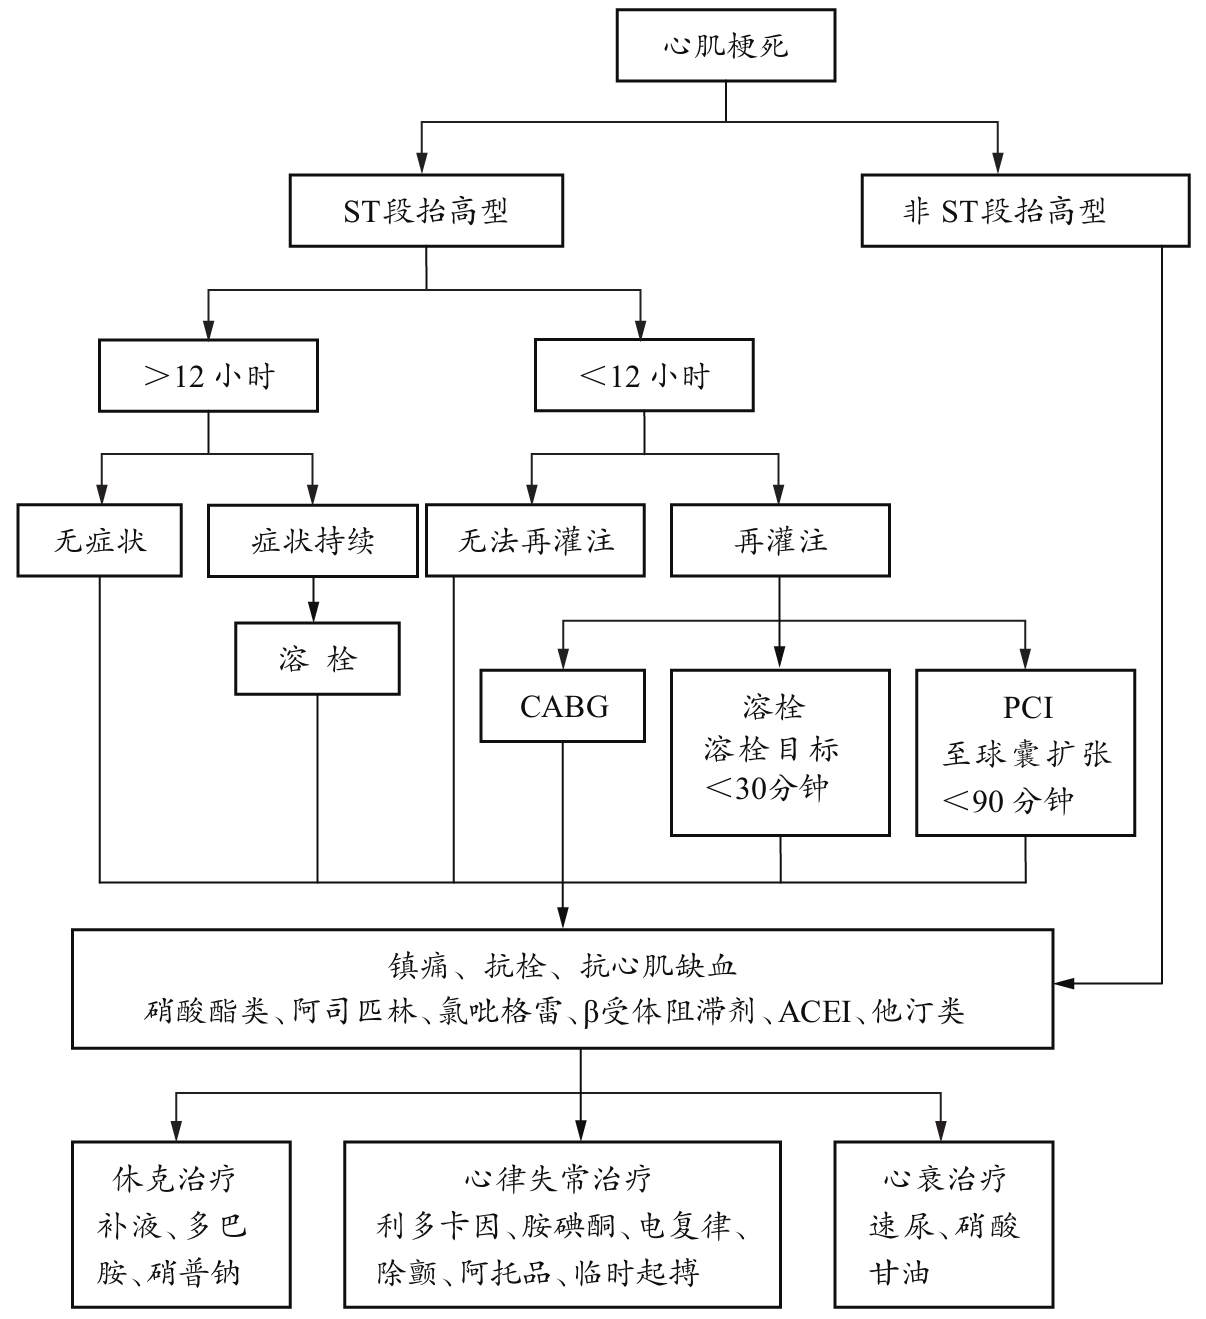
\includegraphics{./images/Image00072.jpg}
 \captionsetup{justification=centering}
 \caption{心肌梗死的治疗程序}
 \label{fig2-5-1}
  \end{figure} 

【治疗方案】

1. 监护和一般治疗

(1)休息:急性期卧床休息1\textasciitilde{}3日,通常第2日可允许患者坐在床旁排便,第3日在病房内走动;梗死后第4\textasciitilde{}5日,逐步增加活动直至每日3次步行100\textasciitilde{}150米。病情不稳定及高危患者卧床时间可适当延长。

(2)监测:进行心电图、血压和呼吸的监测,除颤仪应随时处于备用状态。严重心脏泵衰竭患者应监测肺毛细血管压(PCWP)和静脉压。

(3)吸氧:呼吸困难、血氧饱和度低者,最初数日间断或持续鼻导管、面罩吸氧,有严重低氧血症,需面罩加压给氧或气管插管并机械通气。

2. 镇痛治疗

(1)可予吗啡3mg静脉注射,必要时5分钟重复1次,总量不宜超过15mg;哌替啶50\textasciitilde{}100mg肌内注射,必要时1\textasciitilde{}2小时后再注射1次,以后每4\textasciitilde{}6小时可重复应用。

(2)胸痛较轻者,给予罂粟碱0.03\textasciitilde{}0.06g,肌内注射或口服。

(3)硝酸甘油0.5mg或硝酸异山梨酯5\textasciitilde{}10mg舌下含用或静脉滴注,静脉滴注硝酸甘油应从低剂量(5\textasciitilde{}10μg/min)开始,酌情加量直至症状控制。

(4)心肌再灌注治疗,可有效解除胸疼痛。

3.
再灌注治疗 起病3\textasciitilde{}6小时内,心肌再灌注治疗可使濒临坏死心肌得以存活,或使坏死心肌范围缩小。对ST段抬高急性心肌梗死,及早实施心肌再灌注治疗很重要。通常应在到达医院后30分钟内开始溶栓,或90分钟内接受PCI。

(1)溶栓治疗:发病12小时内,对不具备实施急诊PCI、不能迅速转运、无溶栓禁忌证的STEMI患者,均应在患者就诊30分钟内实施溶栓治疗。

适应证:①两个或两个以上相邻导联ST段抬高(胸导联≥0.2mV,肢导联≥0.1mV),或病史提示AMI伴左束支传导阻滞,起病时间\textless{}12小时,患者年龄\textless{}75岁。②STEMI患者,≥75岁,权衡利弊后仍可考虑。③STEMI,发病时间12\textasciitilde{}24小时,仍有进行性缺血性胸痛者,广泛ST段抬高者也可考虑。

禁忌证:①以往脑出血病史,脑血管结构异常(如动静脉畸形),6个月内缺血性卒中或短暂性脑缺血史(不包括3小时内的缺血性卒中);②颅内肿瘤;③近期(2\textasciitilde{}4周)有活动性内脏出血;④疑诊主动脉夹层;⑤未控制的严重高血压(\textgreater{}180/110mmHg)或慢性严重高血压病史;⑥已知使用治疗剂量的抗凝剂有出血倾向;⑦近期(2\textasciitilde{}4周)创伤史,包括头部外伤、创伤性心肺复苏或持续10分钟以上的心肺复苏;⑧近期3周内外科大手术;⑨2周内出现不能压迫部位的大血管行穿刺术;⑩感染性心内膜炎、妊娠、活动性消化性溃疡。

溶栓药物:①非特异性纤溶酶原激活剂:如尿激酶、链激酶,对血栓部位或体循环中纤溶系统均有作用。尿激酶(UK):150万U溶于100ml生理盐水,30分钟内静脉滴注。链激酶(SK)或重组链激酶(rSK)150万U,60分钟内静脉滴注,用链激酶时,注意寒战、发热、过敏反应等。②组织性纤溶酶原激活剂:人重组型组织纤维蛋白溶酶原激活剂(rt-PA)、阿替普酶,其他特异性纤溶酶原激活剂,采用基因工程改良的组织纤溶酶原激活剂衍生物,溶栓治疗的选择性更高,有瑞替普酶、兰替普酶和替奈普酶等。阿替普酶,全量90分钟加速给药法,首先静脉推注15mg,随后以0.75mg/kg在30分钟内持续静脉滴注(最大剂量不超过50mg),继之0.5mg/kg于60分钟持续静脉滴注(最大剂量不超过35mg);也可半量给药,其血管再通率相对偏低。50mg溶于50ml专用溶剂,首先静脉推注8mg,而后42mg于90分钟内滴完。瑞替普酶10U溶于5\textasciitilde{}10ml注射用水,2分钟以上静脉推注,30分钟后重复上述剂量。替奈普酶,一般为30\textasciitilde{}50mg溶于10ml生理盐水静脉推注。根据体重调整剂量:如体重\textless{}60kg,剂量为30mg;体重每增加10kg,剂量增加5mg,最大剂量为50mg。③溶栓期间辅助抗凝治疗参见“抗栓和抗心肌缺血治疗”。

(2)经皮冠状动脉介入治疗(PCI):

直接PCI:及早实施PCI有助于挽救心肌与生命,从就诊至球囊扩张时间应少于90分钟,对出现症状12小时内的STEMI、伴有新出现的左束支传导阻滞患者,应及早行直接PCI;对于STEMI并发心源性休克、非STEMI,但梗死相关动脉严重狭窄也可选择直接PCI。

转运PCI:高危STEMI患者就诊于无PCI条件的医院,有溶栓禁忌证,虽无溶栓禁忌证但发病超过3小时,可在抗栓治疗同时,尽快转运患者至可行PCI医院。

溶栓后紧急PCI:发病后已经采取溶栓治疗36小时内的心源性休克,或发病12小时内严重心力衰竭和(或)肺水肿(KillipⅢ级);溶栓治疗后仍有持续心肌缺血的高危患者可行紧急PCI。

择期PCI:早期溶栓治疗成功或未溶栓患者,心肌梗死再发、心肌缺血表现、心源性休克、心力衰竭、严重心律失常者,在病情稳定7\textasciitilde{}14日后(危重者可延长时间)行冠状动脉造影,必要时可行PCI治疗。

(3)冠状动脉旁路移植术(CABG):介入治疗失败或溶栓治疗无效而有手术指征者,宜在6\textasciitilde{}8小时内施行CABG。机械性并发症(如心室游离壁破裂、乳头肌断裂、室间隔穿孔)引起心源性休克时,需在急性期行CABG和相应心脏手术治疗。

4. 抗栓治疗

(1)抗血小板治疗:

阿司匹林:无禁忌证者立即嚼服肠溶阿司匹林300mg,然后以100mg/d长期口服。

二磷酸腺苷(ADP)受体拮抗剂:氯吡格雷首次负荷量300mg(拟直接PCI者600mg),以后以75mg/d维持。未置入支架者,应使用氯吡格雷75mg/d至少28日。因急性冠状动脉综合征接受支架置入者,术后使用氯吡格雷75mg/d至少12个月。

血小板膜糖蛋白Ⅱb/Ⅲa(GPⅡb/Ⅲa)受体拮抗剂:静脉溶栓联合GPⅡb/Ⅲa受体拮抗剂可提高疗效,但出血并发症增加。在双抗血小板治疗及有效抗凝治疗时,不推荐常规应用GPⅡb/Ⅲa受体拮抗剂。在直接行PCI的STEMI患者,术后可静脉使用阿昔单抗、依替非巴肽和替罗非班。阿昔单抗,静脉推注0.25mg/kg,再以0.125\textasciitilde{}10μg/(kg·min)维持静脉滴注12小时。依替非巴肽,先静脉推注180μg,10分钟后再推注180μg,再以2μg/(kg·min)静脉滴注12\textasciitilde{}24小时。替罗非班,静脉推注负荷量25μg/kg,再以0.15μg/(kg·min)维持静脉滴注24小时。

(2)抗凝治疗:

普通肝素:rt-PA溶栓前先静脉注射肝素60U/kg(最大量4000U),继以12μg/(kg·h)(最大1000U/h),使APTT值维持在对照值1.5\textasciitilde{}2.0倍,至少应用48小时。尿激酶和链激酶为非选择性溶栓剂,无需充分抗凝治疗,溶栓后6小时开始测定APTT或活化凝血时间(ACT),待其恢复到对照时间2倍以内时开始给予皮下肝素治疗。溶栓期间溶栓结束后6\textasciitilde{}12小时后皮下注射普通肝素7500U,共3\textasciitilde{}5日。若需用GPⅡb/Ⅲa受体拮抗剂,肝素剂量需酌情减量。

低分子量肝素:具有应用方便、无需监测凝血时间、血小板减少症的发生率低等优点,建议用低分子量肝素代替普通肝素。依诺肝素,年龄\textless{}75岁,血肌酐≤221μmol/L(2.5mg/dl)(男),或≤177μmol/L(2.0mg/dl)(女)者,先静脉推注30mg,15分钟后开始1mg/kg皮下注射,12小时1次,直至出院,最长使用8日;≥75岁者,不用静脉负荷量,直接0.75mg/kg皮下注射,12小时1次,最长使用8日。肌酐清除率\textless{}30ml/min者,给予1mg/kg皮下注射,24小时1次。

磺达肝癸钠:属于间接Xa因子抑制剂,有利于降低死亡和再梗死发生率,不增加出血并发症。初始静脉注射2.5mg,随后每日2.5mg皮下注射1次,最长8日。

5. 抗心肌缺血和其他治疗

(1)硝酸酯类:包括硝酸甘油、硝酸异山梨酯和5-单硝山梨醇酯(用法参见“不稳定心绞痛”)。

(2)β受体阻滞剂:如无禁忌证可尽早使用美托洛尔、卡维地洛等,尤其是前壁心肌梗死伴有交感神经功能亢进者,缩小梗死范围。美托洛尔静脉注射每次5mg,必要时可再给予1\textasciitilde{}2次,如心率\textless{}60次/分,收缩压\textless{}100mmHg,应停止静脉给药。口服酒石酸美托洛尔每次25\textasciitilde{}50mg,每6\textasciitilde{}8小时1次,若患者耐受良好,可转换为相应剂量的长效控释制剂。

(3)ACEI和ARB:ACEI无禁忌证者从小剂量开始逐渐增加至目标剂量,如卡托普利(起始6.25mg,然后12.5\textasciitilde{}25mg,每日2次)。不能耐受ACEI者可选用ARB类制剂。

(4)钙通道阻滞剂:STEMI患者不推荐使用短效二氢吡啶类钙拮抗剂;对无左心室收缩功能不全或AVB的STEMI患者,为缓解心肌缺血、控制房颤或心房扑动的快速心室率,如果β受体阻滞剂无效或有禁忌证时,可应用非二氢吡啶类钙拮抗剂。STEMI后合并严重心绞痛时,在β受体阻滞剂基础上可加用地尔硫䓬
。STEMI合并难治性高血压,在ACEI和β受体阻滞剂基础上,加用长效二氢吡啶类钙拮抗剂。

(5)他汀类药物:除调脂作用外,他汀类药物还具有抗炎、改善内皮功能、抑制血小板聚集等,所有无禁忌证的STEMI患者入院后应尽早开始他汀类药物治疗。

6. 抗心律失常治疗

(1)室性心律失常:

室性早搏:对无症状室性早搏,无需抗心律失常药物治疗。

室性逸搏心律:急性STEMI早期常见。除非心率过缓,一般无需特殊处理。

室速和室颤:非持续性室速(持续时间\textless{}30秒且无明显血流动力学异常者)和加速性室性自主心律,通常无需预防性使用抗心律失常药物。多形性室速、持续性单形性室速伴有血液动力学不稳定时应给予同步直流电复律。血流动力学稳定的室速可静脉注射利多卡因、胺碘酮、索他洛尔等。①胺碘酮首剂75\textasciitilde{}150mg稀释于20ml生理盐水中,10分钟内静脉注入;继之以1mg/min静脉滴注6小时,后改为0.5mg/min,总量小于1200mg/d;静脉用药2\textasciitilde{}3日后改为口服,每日0.6\textasciitilde{}0.8g,1周后减为0.1\textasciitilde{}0.4g/d。②利多卡因50\textasciitilde{}100mg静脉注射,每5\textasciitilde{}10分钟重复1次,至期前收缩消失或总量已达300mg,继以1\textasciitilde{}3mg/min静脉滴注维持(100mg加入5\%葡萄糖液100ml,滴注1\textasciitilde{}3ml/min),稳定后可给予美西律150\textasciitilde{}200mg,每6\textasciitilde{}8小时1次。③索他洛尔首剂1\textasciitilde{}1.5mg/kg,以5\%葡萄糖20ml稀释,15分钟内注入,疗效不明显可重复1次,后改为口服160\textasciitilde{}640mg/d。室颤或持续多形性室性心动过速时,立即非同步直流电除颤或同步直流电复律。单形性室性心动过速药物疗效不佳时,也应及早同步直流电复律。

(2)对缓慢性心律失常:可用阿托品0.5\textasciitilde{}1mg肌内或静脉注射。Ⅱ\textasciitilde{}Ⅲ度房室传导阻滞,伴血流动力学障碍、心脏停搏者宜用临时起搏器治疗。

(3)室上性快速心律失常:选用维拉帕米、地尔硫䓬
、美托洛尔、洋地黄制剂、胺碘酮等药物治疗,不能控制时,可考虑用同步直流电复律治疗。

7.
心源性休克的治疗 根据单纯心源性休克,或有周围血管舒缩障碍或血容量不足等因素存在,而分别处理。

(1)补充血容量:血容量不足或中心静脉压和肺动脉楔压低者,用右旋糖酐或5\%\textasciitilde{}10\%葡萄糖液静脉滴注,输液后如中心静脉压上升\textgreater{}18cmH{2}
O,肺小动脉楔压\textgreater{}15\textasciitilde{}18mmHg,则应停止。右心室梗死时,中心静脉压升高并非是补充血容量的禁忌证。

(2)应用升压药:若补液1000\textasciitilde{}2000ml血压仍不升,而肺小动脉楔压和心排血量正常时,可用多巴胺起始剂量3\textasciitilde{}5μg/(kg·min),或多巴酚丁胺起始剂量2.5\textasciitilde{}5μg/(kg·min),亦可选用去甲肾上腺素2\textasciitilde{}8μg/min静脉滴注。

(3)应用血管扩张剂:经上述处理血压仍不升,而肺动脉楔压(PCWP)高,心排血量低或周围血管显著收缩以致四肢厥冷并有发绀时,硝普钠15μg/min开始静脉滴注,每5分钟逐渐增量至PCWP降至15\textasciitilde{}18mmHg;硝酸甘油10\textasciitilde{}20μg/min开始静脉滴注,每5\textasciitilde{}10分钟增加5\textasciitilde{}10μg/min直至左室充盈压下降。

(4)其他措施:包括纠正酸中毒和电解质紊乱,避免脑缺血、保护肾功能,必要时应用洋地黄制剂等。为了降低心源性休克的病死率,条件允许时考虑用主动脉内球囊反搏术(IABP)进行辅助循环,然后作选择性冠状动脉造影,及时实施PCI或CABG可挽救部分患者的生命。

8.
治疗心力衰竭 主要是治疗急性左心衰竭,利尿剂可降低左室充盈压力,一般有效,亦可选用血管扩张剂如硝酸甘油静脉滴注减轻心脏前后负荷,或用多巴酚丁胺10μg/(kg·min)静脉滴注或用短效血管紧张素转换酶抑制剂从小剂量开始等治疗。洋地黄制剂可能引起室性心律失常,在梗死发生后24小时内宜尽量避免使用。右心室梗死患者应慎用利尿剂。

9. 其他治疗

(1)极化液疗法:氯化钾1.5g、胰岛素10U加入10\%葡萄糖液500ml中,静脉滴注,每日1\textasciitilde{}2次,7\textasciitilde{}14日为一个疗程。可减少心律失常,为缺血心肌提供代谢支持。

(2)中医中药治疗:四逆汤、独参汤或参附汤对心梗伴低血压或休克有一定疗效,患者如兼有阴虚表现可用参脉散。

10.
并发症的治疗 并发栓塞时可予抗凝治疗。室壁瘤形成伴心力衰竭或引起严重心律失常可考虑手术切除或同时作主动脉冠状动脉旁路移植手术。心脏破裂和乳头肌功能严重失调都可考虑手术治疗,但手术死亡率高。心肌梗死后综合征可用糖皮质激素或阿司匹林、吲哚美辛等治疗。

11.
右心室心肌梗死的处理 治疗措施与左心室MI略有不同。右心室心肌梗死引起右心衰竭伴低血压,而无左心衰竭的表现时,治疗宜补充血容量。在血流动力学监测下静脉滴注输液,直到低血压得到纠治或肺毛细血管压达15\textasciitilde{}18mmHg。若低血压仍未能纠正,可用正性肌力药如多巴酚丁胺。利尿药和硝酸酯类可能引起严重的低血压,临床应相对禁忌使用。伴有房室传导阻滞者可予以临时起搏。

12.
非ST段抬高性心肌梗死的处理 非ST段抬高性MI通常为非Q波性,此类患者不宜溶栓治疗。其中,低危患者如无合并症、血流动力异常、不伴反复胸痛者,以抗凝及抗血小板为主;中危患者,如伴持续或反复胸痛、心电图无变化或ST段压低1mm者,及高危患者包括并发心源性休克、肺水肿或持续低血压者,则以介入治疗为首选。其余治疗原则同上。

【疗效观察与随访】

1.
观察指标 心电图、心肌酶谱、血象、临床症状与体征等。溶栓治疗时注意出凝血指标。

2.
治愈标准 症状消失,心电图回复正常,心功能正常,心肌酶谱正常,3个月内未复发。

3. 随访 密切观察病情变化,1年内定期复查心电图、心肌酶谱及肝肾功能。

【治疗经验与解析】

1.
镇痛时首选吗啡,除了镇痛作用外,还有扩张血管,减轻心脏负荷和降低心脏耗氧量。副作用主要是呼吸抑制、低血压。如出现呼吸抑制,可予纳洛酮0.4\textasciitilde{}0.8mg拮抗;出现低血压时,很少需要使用升压药,取仰卧或静脉滴注生理盐水。

2.
患者就诊早(发病≤3小时),不能及时进行介入治疗者,或虽具备急诊PCI治疗条件,就诊至球囊扩张时间与就诊至溶栓开始时间相差\textgreater{}60分钟,且就诊至球囊扩张时间\textgreater{}90分钟者应优先考虑溶栓治疗。在发病3小时内行溶栓治疗,梗死相关血管的开通率增高,病死率明显降低,其临床疗效与直接PCI相当。发病3\textasciitilde{}12小时内行溶栓治疗,其疗效不如直接PCI,发病12\textasciitilde{}24小时内,仍有持续或间断缺血症状和持续ST段抬高,也可考虑溶栓治疗。

3.
溶栓主要并发症是出血,尤其是颅内出血,应立即停用溶栓剂,同时降低颅内压,包括适当控制血压、抬高床头30°、静脉滴注甘露醇、气管插管和辅助通气,必要时外科脑室造口术、颅骨切除术以及抽吸血肿等。还可使用逆转溶栓、抗血小板和抗凝的药物:24小时内每6小时给予新鲜冰冻血浆2U;4小时内使用过普通肝素患者,推荐用鱼精蛋白中和(1mg鱼精蛋白中和100U普通肝素);如果出血时间异常,可输入6\textasciitilde{}8U血小板。

4.
PCI时应注意 ①由有经验者施术,以避免延误时机;②发病12小时以上不宜施行PCI;③不宜对非“罪犯”动脉施行PCI;④有心源性休克者宜先行主动脉内球囊反搏术,待血压稳定后再施手术。

5.
急性缺血心肌再灌注时,出现再灌注损伤,表现为再灌注性心律失常。各种快速、缓慢性心律失常均可出现,应作好抢救准备。出现严重心律失常情况少见,最常见非持续性室性心动过速,不必行特殊处理。

6.
心肌梗死合并室性心律失常,应寻找和治疗导致室性心律失常的原因。血钾低者可静脉或口服补钾,也可用硫酸镁来治疗复杂性室性心律失常;早期用β受体阻滞剂可降低室性心律失常的发生率;预防性应用利多卡因可能增加死亡风险,目前不主张使用。

7.
加强二级随访 出院后适度参加体力活动,在医生指导下坚持服药,控制饮食,改变不良的生活习惯,戒烟、戒酒,限制高胆固醇摄入,注意防治高血压、高血脂和糖尿病。

{(四)缺血性心肌病}

缺血性心肌病(ischemic
cardiomyopathy)是指由于冠心病的病理基础导致心肌纤维化(或称硬化)。为心肌的长期血供不足,心肌组织发生营养障碍和萎缩,或大面积MI后,纤维组织增生所致。其临床特点是心脏逐渐扩大,发生心律失常和心力衰竭。因此与扩张型心肌病颇为相似,故被称为缺血性心肌病。

【治疗方案】

1. 预防在于积极防治动脉粥样硬化。

2. 改善冠状动脉供血和心肌营养。

3.
对心力衰竭按一般慢性收缩期心力衰竭的治疗原则,改善心室重构,应用ACEI(或ARB)、β受体阻滞剂、利尿剂或加用地高辛。

4.
对于既往有血栓栓塞病史、心力衰竭、心脏明显扩大、心房颤动或超声心动图证实有附壁血栓形成应给予抗凝。常用阿司匹林85\textasciitilde{}325mg/d,或使用华法林2.5mg/d,据凝血酶原时间的国际标准比值(PT-INR)调整剂量,使PT-INR保持在2\textasciitilde{}3。

5.
病态窦房结综合征和房室传导阻滞而有阿-斯综合征发作者,及早安置永久性人工心脏起搏器;心房颤动患者,如转复窦性心律,应注意合并病态窦房结综合征的可能,以免转复窦性心律后,心率缓慢引起不利后果。发生严重室性心律失常者,除药物治疗外,还可考虑埋藏式自动复律除颤器治疗。

6. 终末期缺血性心肌病患者是心脏移植的主要适应证之一。

【疗效观察与随访】

1. 观察指标 症状与体征,心电图、心功能、超声心动图等。

2.
治愈标准 水肿消失,心率、心律正常,心电图恢复正常半年以上,无并发症。

好转标准 水肿减轻,心电图有改善,心律规整。

3. 随访 定期复查心电图、超声心动图、心功能,随访病情变化。

【治疗经验与解析】

1.
本病是一种持续进展性病变,必须及时采取有效措施以阻止其发展。近年来认为,高度β{1}
选择性的β受体阻滞剂卡维地洛12.5\textasciitilde{}100mg/d,与传统治疗措施合用疗效较好。如琥珀酸美托洛尔23.75\textasciitilde{}190mg/d。

2.
应用曲美他嗪可改善呼吸困难,解除残留的心绞痛症状并减少对其他辅助治疗的需要。

3. 有相应指征的,可行PCI或CABG。

4.
心脏移植虽为终末期的主要适应证,但由于供体缺乏,因而选用时必须极其慎重。


\section{晕厥}

晕厥是一种症状,为短暂的、自限性的意识丧失,常常导致晕倒。晕厥的发生机制是短暂脑缺血,发生较快,随即自动完全恢复。有些晕厥有先兆症状,无先兆症状的突发性意识丧失更多见。通常随着晕厥恢复,行为和定向力也立即恢复。有时可出现逆行性遗忘,多见于老年患者。有时晕厥恢复后可有明显乏力。典型的晕厥发作是短暂的,血管迷走神经性晕厥的意识完全丧失的时间一般不超过20秒。个别晕厥发作时间较长可达数分钟,应与其他原因造成的意识丧失相鉴别。

晕厥主要分三类:①神经反射性晕厥,包括血管迷走神经性晕厥,如情绪异常包括恐惧、疼痛、医疗器械检查、晕血引起的晕厥及立位性晕厥;情境性晕厥,如咳嗽、打喷嚏、胃肠道刺激、排尿后、运动后、饱餐后等;颈动脉窦性晕厥;非典型性晕厥诱因不明和/或症状不典型。②直立性低血压性晕厥,包括原发自主神经异常性晕厥,如单纯自主神经衰竭、多系统萎缩、帕金森病合并自主神经衰竭、痴呆等;继发性自主神经异常性晕厥,如糖尿病、淀粉样变性、尿毒症、脊髓损伤等;药物致体位性低血压,如酒精、血管扩张剂、利尿剂、噻嗪类药物、抗抑郁剂等;血容量不足,如出血、腹泻、呕吐等。③心源性晕厥,包括:心律失常,如心动过缓、慢快综合征、房室交界区异常、辅助器械装置故障、室上性或室性心动过速、药物性心律失常等;器质性病变,如心血管疾病、急性心肌梗死/缺血、肥厚性心肌病、心房粘液瘤、心包疾病/填塞、先天性冠状动脉异常等,其他如肺栓塞、急性主动脉夹层、肺动脉高压。

【治疗程序】 如图\ref{fig2-6-1}所示。

\begin{figure}[!htbp]
 \centering
 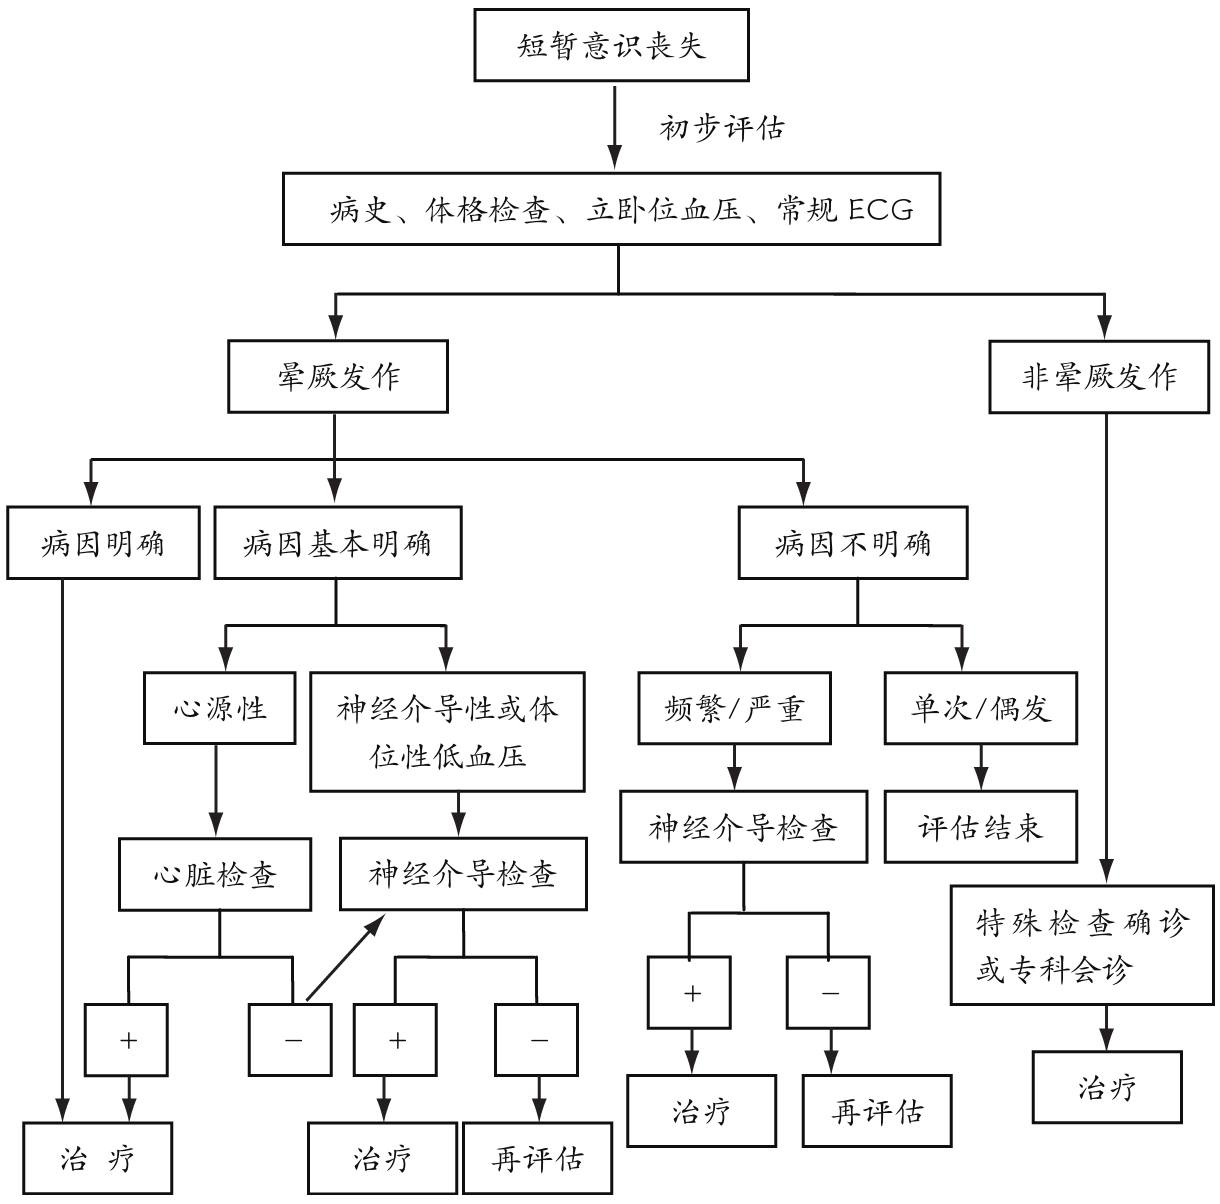
\includegraphics{./images/Image00073.jpg}
 \captionsetup{justification=centering}
 \caption{晕厥的治疗程序}
 \label{fig2-6-1}
  \end{figure} 

【治疗方案】

1. 反射性(血管迷走神经性、情景性、颈动脉窦性)晕厥

(1)物理治疗:已成为治疗反射性晕厥的一线方案,临床试验显示,物理抗压力训练如交叉腿或握力训练能显著升高先兆晕厥者的血压,从而能在多数情况下避免或延迟晕厥发生。对体位诱发因素高度敏感的反复血管神经性晕厥者,逐渐延长站立时间(亦称“倾斜训练”)可减少晕厥发作;但短期倾斜训练并不能降低复发率。

(2)药物治疗:

α受体激动剂:因反射性晕厥患者的周围血管不能适时适度收缩,故有学者认为可用α受体激动剂(依替福林和米多君)。研究证实,依替福林并不能降低晕厥发作频率与次数,而米多君能显著降低晕厥的发生率,而对尿量有不利影响,老年男性患者应慎用。另有研究显示,反射性晕厥单用α受体激动剂疗效不理想,偶有晕厥者不推荐长期应用。

β受体阻滞剂:用于治疗血管迷走神经性晕厥,其主要机制在于负性肌力作用,降低静脉回流量时突然减少时压力感受器的活性,该理论尚未得到临床证实。β阻滞剂还可能会加重颈动脉窦综合征患者的心动过缓,5项长期随访研究显示该类药物对神经反射性晕厥无效。故目前不推荐使用β受体阻滞剂(Ⅲ类,A级)。

(3)心脏起搏:起搏治疗对心脏抑制引起的血管迷走神经性晕厥有效,以血管抑制为主者效差。除严重自发性心动过缓外,反射性晕厥的起搏治疗效果不明显。

2. 直立性低血压和体位性晕厥

(1)健康教育加上改变生活方式可明显改善体位性低血压的症状。动态血压监测有助于了解全天不同环境下的血压变化、药物对患者卧位或夜间血压的影响。

(2)药物诱发的自主神经异常性晕厥首先停药,无高血压者可采取扩充血容量如摄取足够盐和水(每日摄入2\textasciitilde{}3升水和10g氯化钠);快速摄入冷开水对运动中或餐后低血压者有明显疗效;高枕位睡眠(头部抬高10o)可防止夜间多尿,维持适量的体液量及改善夜间高血压。老年患者可佩戴腹带或加压弹力袜以减轻下肢血液蓄积;有先兆晕厥时可采取交叉腿和蹲位姿势等预防措施。

(3)α受体激动剂是慢性自主神经异常者的首选药物。氟氢可的松(每日0.1\textasciitilde{}0.3mg)可促进钠水潴留及扩张血容量,改善晕厥症状。其他治疗如去氨加压素用于伴夜尿增多者;奥曲肽用于餐后低血压,促红细胞生成素用于贫血者等。

3. 心律失常性晕厥

(1)窦房结功能不全伴缓慢心律失常或SNRT异常引起的晕厥,首先停用加重或诱发心动过缓的药物,如无合适的替代药物应行心脏起搏。起搏治疗可明显缓解症状,但对生存率无影响。

(2)房室传导阻滞引起的晕厥需起搏治疗,永久右室心尖部起搏的危害已得到证实,但其替代起搏位点仍存争议。房室传导阻滞伴射血分数下降、心力衰竭及QRS间期延长所致的晕厥可采用双腔起搏。

(3)阵发性室上性和室性心动过速或典型房扑引起的晕厥应首选导管消融术。尖端扭转型室速所致的晕厥主要是应用延长QT间期的药物所致,应立即停药。心功能正常或轻度受损者,出现室性心动过速伴晕厥,考虑导管消融或药物治疗。心功能不全、室性心动过速或室颤伴晕厥,且病因无法去除者应植入ICD。尽管ICD不能有效预防晕厥复发,但可降低猝死风险,其适应证包括:①明显室速及器质性心脏病者(Ⅰ类,B级);②既往有心肌梗死、电生理检查显示持续单型室速者(Ⅰ类,B级);③明显室速伴遗传性心肌疾病或离子通道异常者(Ⅱa类,B级)。

4.
继发于器质性心脏病或心血管疾病性晕厥 严重主动脉狭窄或心房粘液瘤所致的晕厥可考虑手术治疗;继发于急性心血管事件如肺栓塞、心肌梗死或心包填塞者主要采取病因治疗;大多数心肌缺血所致者可采用药物和(或)血管重建;由原发性肺动脉高压或限制性心肌病引起者,一般不易纠正原发病。

5. 有猝死高危因素伴原因不明性晕厥

(1)急、慢性冠状动脉疾病或左室射血分数下降均可增加死亡风险,故有必要评估缺血的严重程度,如有适应证应考虑血运重建。但血运重建并不能改善恶性心律失常引起的不良后果,因此该类患者应行电生理检查以评估有无心律失常。心力衰竭且符合最新指南制定的ICD适应证者,无论晕厥发生机制是否明确,均应植入ICD。研究显示,植入ICD的晕厥患者生存率明显增加;不明原因晕厥的缺血性或非缺血性心肌病伴心衰或LVEF严重下降者应植入ICD(Ⅰ类,A级);左室射血分数正常和电生理检查阴性者不建议植入ICD。

(2)肥厚型心肌病伴不明原因晕厥尤其发作间期短(\textless{}6个月)、相对危险度\textgreater{}5,其猝死风险性较高;植入ICD效果明显。

(3)约1/3致心律失常性右室心肌病(ARVC)者会发生晕厥。年轻、严重右室发育不全、左室功能障碍、多形性室性心动过速、心室晚电位、epsilon波及有猝死家族史者,如无其他病因应考虑植入ICD。

(4)遗传性离子通道异常性心脏病常以晕厥为先兆表现,该类患者是否应植入ICD仍存争议。

【疗效观察与随访】

1. 观察指标

(1)心源性晕厥:密切观察心率、心律变化,及时检查心电图,必要时进行心电监测。

(2)血源性晕厥:密切观察血糖、血气及电解质变化,必要时进行血气监测、血糖监测。

(3)血管源性晕厥:密切观察血压、脉搏变化,必要时进行心电监护。

(4)反射性晕厥:询问出现的原因及情况,加强教育与预防,常因人、因情况而异。

(5)情景性晕厥:注意发作情景,消除诱发因素。

2.
治愈标准 神志清楚,生命体征恢复正常,各项相关检查指标恢复正常,1周内未复发。

3. 随访 1周内围绕病因进行复查,特别注意病情有无复发。

【治疗经验与解析】

1.
物理抗压力训练、健康教育及避免诱发因素有助于血管迷走神经性晕厥的治疗。在干预生活方式、抗压力训练后,症状仍未改善者,考虑倾斜训练,特别适用于年轻、症状严重及对诱发因素高度敏感者。

2.
情景性晕厥患者,祛除或避免诱因很重要;如果诱因难以祛除,应适当补充血容量、保持适当体位。

3. 以心脏抑制为主的颈动脉窦综合征 患者可考虑心脏起搏(Ⅱ{a}
类,B级);反复神经性晕厥、年龄\textgreater{}40岁及心电监测显示以心脏抑制为主者也可考虑心脏起搏(Ⅱ{a}
类,B级);倾斜试验出现心脏抑制反应、频发无先兆晕厥、年龄\textgreater{}40岁且改变治疗方案无效者可考虑心脏起搏(Ⅱ{b}
类,C级);非心脏抑制为主的反射性晕厥,不推荐起搏治疗(Ⅲ类,C级)。


\section{高血压}

\subsection{高血压病}

原发性高血压(primary
hypertension)是指排除了各种继发因素,以血压升高为主要临床表现伴或不伴有多种心血管危险因素的综合征,通常简称为高血压病。高血压是多种心、脑血管疾病的重要病因和危险因素,影响重要脏器,如心、脑、肾的结构与功能,最终导致器官功能衰竭。高血的压定义为,诊室测量收缩压≥140mmHg和(或)舒张压≥90mmHg,根据血压升高水平,进一步将高血压分为1\textasciitilde{}3级。24小时动态血压监测,平均血压≥130/80mmHg。左、右上臂血压分别相差小于10\textasciitilde{}20mmHg和10mmHg,右侧高于左侧。下肢高于上肢,血压相差20\textasciitilde{}40mmHg。临床上原发性高血压多有遗传因素、高龄、高盐饮食、肥胖、吸烟、饮酒、精神紧张、缺乏运动、对常规降压药有降压反应等病史。

【治疗程序】 根据血压分级、心血管危险因素、糖尿病、靶器官损害以及并发症情况,将高血压患者分为低危、中危、高危和很高危(表\ref{tab2-7-1})。

\begin{longtable}[]{@{}lll@{}}
    \caption{不同患者的危险度与治疗程序}
    \label{tab2-7-1}\\
\toprule
危险性分层 & 10年内心血管事件的绝对危险 & 治疗程序\tabularnewline
\midrule
\endfirsthead
\caption[]{不同患者的危险度与治疗程序}\\
\toprule
危险性分层 & 10年内心血管事件的绝对危险 & 治疗程序\tabularnewline
\midrule
\endhead
\bottomrule
\endfoot
低危 & \textless{}15\% &
改变生活行为3\textasciitilde{}6个月,如不达标药物治疗\tabularnewline
中危 & 15\%\textasciitilde{}20\% &
如病情许可,改变生活行为1个月,如不达标药物治疗\tabularnewline
高危 & 20\%\textasciitilde{}30\% &
改变生活行为+强化药物治疗\tabularnewline
很高危 & \textgreater{}30\% & 改变生活行为+强化药物治疗\tabularnewline
\end{longtable}

其他心血管危险因素包括:①男性\textgreater{}55岁,女性\textgreater{}65岁;②吸烟;③血胆固醇(TC)\textgreater{}5.72mmol/L(220mg/dl),或低密度脂蛋白胆固醇(LDL-c)\textgreater{}3.3mmol/L(130mg/dl),或高密度脂蛋白胆固醇(HDL-c)\textless{}1.0mmol/L(40mg/dl);④早发心血管疾病家族史(一级亲属发病年龄\textless{}50岁);⑤腹型肥胖(腹围:男性≥85cm,女性≥80cm),或体质量指数BMI\textgreater{}28kg/m{2}
;⑥高敏C反应蛋白(hs-CRP)≥1mg/dl;⑦缺乏体力活动。

用于分层的靶器官损害:①左心室肥厚(心电图或超声心动图);②颈动脉超声证实有动脉粥样斑块或内膜中层厚度(IMT)≥0.9mm;③血肌酐轻度升高:男性115\textasciitilde{}133μmol/L(1.3\textasciitilde{}1.5mg/dl),女性107\textasciitilde{}124μmol/L(1.2\textasciitilde{}1.4mg/dl);④微量白蛋白尿30\textasciitilde{}300mg/24h,或尿白蛋白/肌酐比值:男性≥22mg/g,女性≥31mg/g。

用于分层的并发症包括心脏疾病如心绞痛、心肌梗死、冠状动脉血运重建、心力衰竭,脑血管疾病如脑出血、缺血性卒中、短暂性脑缺血发作,肾脏疾病如糖尿病肾病、血肌酐升高,男性\textgreater{}133μmol/L或女性\textgreater{}124μmol/L、临床蛋白尿\textgreater{}300mg/24h,血管疾病如主动脉夹层、外周血管病,高血压性视网膜病变如出血或渗出、视乳头水肿。

【治疗方案】

{(一)治疗原则}

1. 从小剂量开始,逐渐增加药物剂量,3个月内降压达标。

2. 选用疗效维持24小时的长效降压药。

3. ≥2级的高血压需联合使用降压药物。

4. 多重心血管危险因素协同控制,个体化治疗。

{(二)血压控制目标值}

1.
应将患者血压降到其能最大耐受水平,通常血压控制目标值至少\textless{}140/90mmHg。

2.
高危人群(糖尿病、冠心病、卒中、慢性肾病)血压控制在\textless{}130/80mmHg,2013年欧洲高血压管理指南改为140/80mmHg。

3.
老年患者血压\textless{}150/90mmHg,老年或冠心病患者舒张压不低于60mmHg。

{(三)非药物治疗}

1. 改善生活方式 是高血压患者降压治疗的基础。

2. 减轻体重 尽量将体质量指数(BMI)控制在\textless{}25。

3. 限制钠盐摄入 每人每日食盐量以不超过6g为宜。

4. 补充钙和钾盐 食用新鲜蔬菜、牛奶。

5. 减少脂肪摄入 膳食中脂肪量应控制在总热量的25\%以下。

6. 戒烟、限制饮酒 饮酒量每日不可超过相当于50g乙醇的量。

7.
增加运动 可根据年龄及身体状况选择慢跑或步行,一般每周3\textasciitilde{}5次,每次30\textasciitilde{}60分钟。

8. 保持心理卫生。

{(四)药物治疗}

1.
降压药物种类 目前常用降压药物可归纳为五大类,即钙通道阻滞剂(CCB)、血管紧张素转换酶抑制剂(ACEI)和血管紧张素Ⅱ{1}
受体阻滞剂(ARB)、利尿剂、β受体阻滞剂。

2.
合理的联合治疗 适用于2级以上高血压以及高危的高血压患者,常见的联合方案有以下几种:

(1)CCB+ACEI:如氨氯地平、尼群地平、硝苯地平+依那普利、贝那普利、培哚普利。

(2)利尿剂+ACEI:如吲达帕胺、氢氯噻嗪+依那普利、贝那普利、培哚普利。

(3)CCB+β受体阻滞剂:如尼群地平+琥珀酸美托洛尔、尼群地平+阿替洛尔。

(4)CCB+利尿剂:如尼群地平+吲达帕胺、氢氯噻嗪、非洛地平+氢氯噻嗪。

(5)3种以上的药物联合:如ACEI+CCB+利尿剂、ARB+CCB+利尿剂。除有禁忌证外,三种降压药合理的联合治疗方案必须包含利尿剂。

3. 各种降压药物作用特点

(1)利尿剂:有噻嗪类、襻利尿剂和保钾利尿剂三类。适用于轻、中度高血压,在盐敏感性高血压、合并肥胖或糖尿病、更年期女性和老年人高血压有较强降压效应。利尿剂的主要不良反应是低血钾症,影响血脂、血糖、血尿酸代谢,推荐使用小剂量。痛风患者禁用,襻利尿剂主要用于肾功能不全时。

(2)β受体阻滞剂:包括选择性(β{1} )、非选择性(β{1} 与β{2}
)和兼有α受体阻滞作用三类。适用于高肾素型,心率较快的中、青年患者或合并心绞痛患者。不良反应主要有心动过缓、乏力、四肢发冷、降低生活质量等。急性心力衰竭、支气管哮喘、病态窦房结综合征、Ⅱ度Ⅱ型房室传导阻滞和外周血管病患者禁用。

(3)钙通道阻滞剂:分为二氢吡啶类和非二氢吡啶类,前者包括硝苯地平、非洛地平、氨氯地平,后者有维拉帕米、地尔硫䓬
。起效迅速、强力,可用于不同程度的高血压,特别适用于老年高血压或合并稳定性心绞痛、高钠低肾素型患者。主要不良反应包括初心率增快、面部潮红、头痛、下肢水肿等,多见于初始治疗阶段,尤其短效制剂时。非二氢吡啶类抑制心肌收缩及自律性和传导性,不宜用于心力衰竭加重期、窦房结功能低下或心脏传导阻滞患者。

(4)血管紧张素转换酶抑制剂:根据化学结构分为巯基、羧基和磷酰基三类。特别适用于伴有心力衰竭、心肌梗死后、糖耐量减退或糖尿病肾病的高血压患者。不良反应主要是刺激性干咳和血管性水肿。高血钾症、妊娠妇女和双侧肾动脉狭窄患者禁用。血肌酐超过3mg患者需慎用。

(5)血管紧张素Ⅱ1型受体拮抗剂:通过拮抗血管紧张素Ⅱ1型受体而发挥降压作用。尽管ACEI与ARB在适应证、禁忌证方面相似,ARB比ACEI的刺激性干咳不良反应少,持续治疗的依从性高。

{(五)有高血压并发症和合并疾病的降压治疗}

1.
脑血管病 可选择ARB、长效钙拮抗剂、ACEI或利尿剂。以单个降压药并从小剂量开始,再缓慢递增剂量或联合治疗。

2.
冠心病 高血压合并稳定性心绞痛的降压治疗,应选择β受体阻滞剂、血管紧张素转换酶抑制剂和长效钙拮抗剂;有心肌梗死病史患者,应选择ACEI和β受体阻滞剂。

3.
心力衰竭 高血压合并无症状左心室功能不全的降压治疗,应选择ACEI和β受体阻滞剂,从小剂量开始。有心力衰竭症状者,加用利尿剂、ACEI或ARB和β阻滞剂联合治疗。

4.
慢性肾衰竭 ACEI或ARB在早、中期能延缓肾功能恶化,要注意在低血容量或病情晚期(肌酐清除率\textless{}30ml/min或血肌酐超过265μmol/L,即3.0mg/dl)可能使肾功能恶化。血液透析患者仍需降压治疗。

5. 糖尿病 ACEI或ARB、长效钙拮抗剂和小剂量利尿剂是较合理的选择。

{(六)顽固性高血压治疗(图\ref{fig2-7-1})}

\begin{figure}[!htbp]
 \centering
 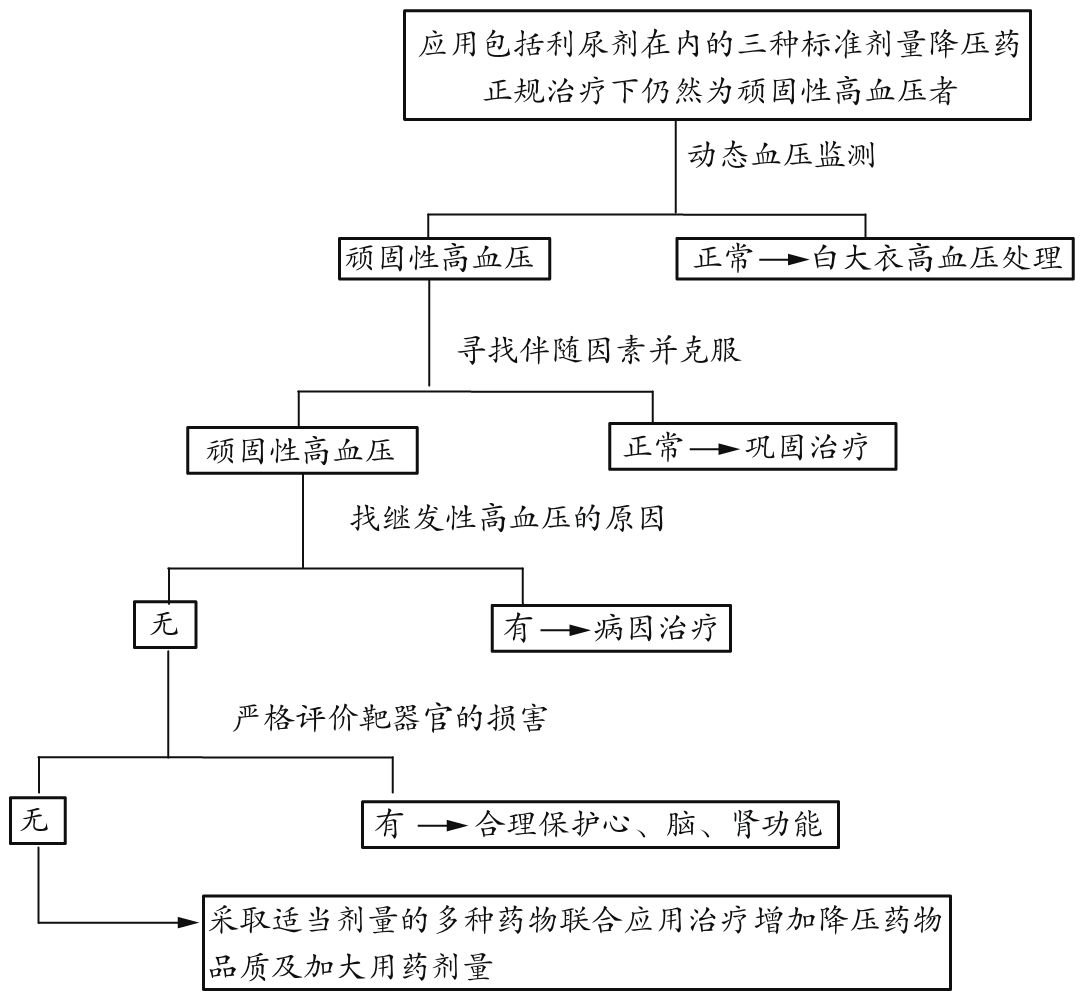
\includegraphics{./images/Image00074.jpg}
 \captionsetup{justification=centering}
 \caption{顽固性高血压治疗程序}
 \label{fig2-7-1}
  \end{figure} 

{(七)高血压危象的处理}

1.
高血压急症 应在数分钟或1小时内将血压降至目标值,一般先降到原来动脉血压的20\%\textasciitilde{}30\%。通常经非胃肠给药,如硝普钠开始时以50mg/500ml浓度每分钟10\textasciitilde{}25μg速率静脉滴注,立即发挥降压作用,可用于各种高血压急症。硝酸甘油开始时以每分钟5\textasciitilde{}10μg速率静脉滴注,然后每5\textasciitilde{}10分钟增加滴注速率至每分钟20\textasciitilde{}50μg。硝酸甘油主要用于急性心力衰竭或急性冠脉综合征时高血压急症。地尔硫䓬
配制成50mg/500ml浓度,以每小时5\textasciitilde{}15mg速率静脉滴注,主要用于高血压危象或急性冠脉综合征。拉贝洛尔开始时缓慢静脉注射50mg,以后可以每隔15分钟重复注射,总剂量不超过300mg,也可以每分钟0.5\textasciitilde{}2mg速率静脉滴注。主要用于妊娠或肾衰竭时高血压急症。

2.
高血压次急症 需在数小时到24小时内降低血压,可使用快速起效的口服降压药。

【疗效观察与随访】

1. 观察指标 血压、血糖、血脂、心电图、临床症状与体征等。

2. 疗效判定

治愈标准:血压连续稳定在正常范围3个月以上,无并发症。

好转标准:血压仍略高,对降压药敏感。

3. 随访

(1)定期随诊:血压达标后,可每3\textasciitilde{}6个月随访1次,有合并症如心力衰竭或伴随其他疾病如糖尿病,应增加随诊频率,随访过程中应注意监测和纠正其他危险因素。每年至少检查1\textasciitilde{}2次血钾和肌酐,随诊过程中还须监测药物的不良反应。

(2)药物剂量的调整和减药:开始给小剂量药物,经过1个月治疗,如血压未达标而不良反应少或可耐受,逐渐增加剂量;如出现不良反应导致不能耐受,改用另一种药物;如患者血压已长期得以控制,可以尝试小心、逐步减少服药次数或剂量。

【治疗经验与解析】

1.
老年人对钙通道拮抗剂敏感,中青年对β受体阻滞剂敏感,如果患者对ACEI或ARB特别敏感,排除严重肾功能损害,应考虑有肾动脉狭窄的可能。

2.
降压起效速度:CCB\textgreater{}利尿剂\textgreater{}β受体阻滞剂\textgreater{}ACEI\textgreater{}ARB。

3.
不同的降压药物联用可产生协同作用,相同的降压药物联合只能在原降压疗效基础上增加20\%。

\subsection{继发性高血压}

继发性高血压又称为症状性高血压,是指由某些确定的疾病或病因引起的血压升高,约占所有高血压的5\%。不少继发性高血压,如原发性醛固酮增多症、嗜铬细胞瘤、肾血管性高血压、肾素分泌瘤等,可通过手术得到根治或改善。及早确诊可明显提高治愈率或阻止病情进展。

【治疗方案】

1.
原发性醛固酮增多症 是肾上腺皮质增生或肿瘤分泌过多醛固酮所致,临床上以长期高血压伴低血钾为特征,少数患者血钾正常,其发病年龄高峰为30\textasciitilde{}50岁,女性多于男性。手术切除腺瘤是其治疗方案。术前给予醛固酮拮抗剂(如螺内酯或依普利酮)。对肾上腺增生,给予醛固酮拮抗剂治疗。治疗程序如图\ref{fig2-7-2}\footnote{PAC---血浆醛固酮浓度;PRA---血浆肾素活性;18-(OH)-B---18羟皮质酮}所示。

\begin{figure}[!htbp]
 \centering
 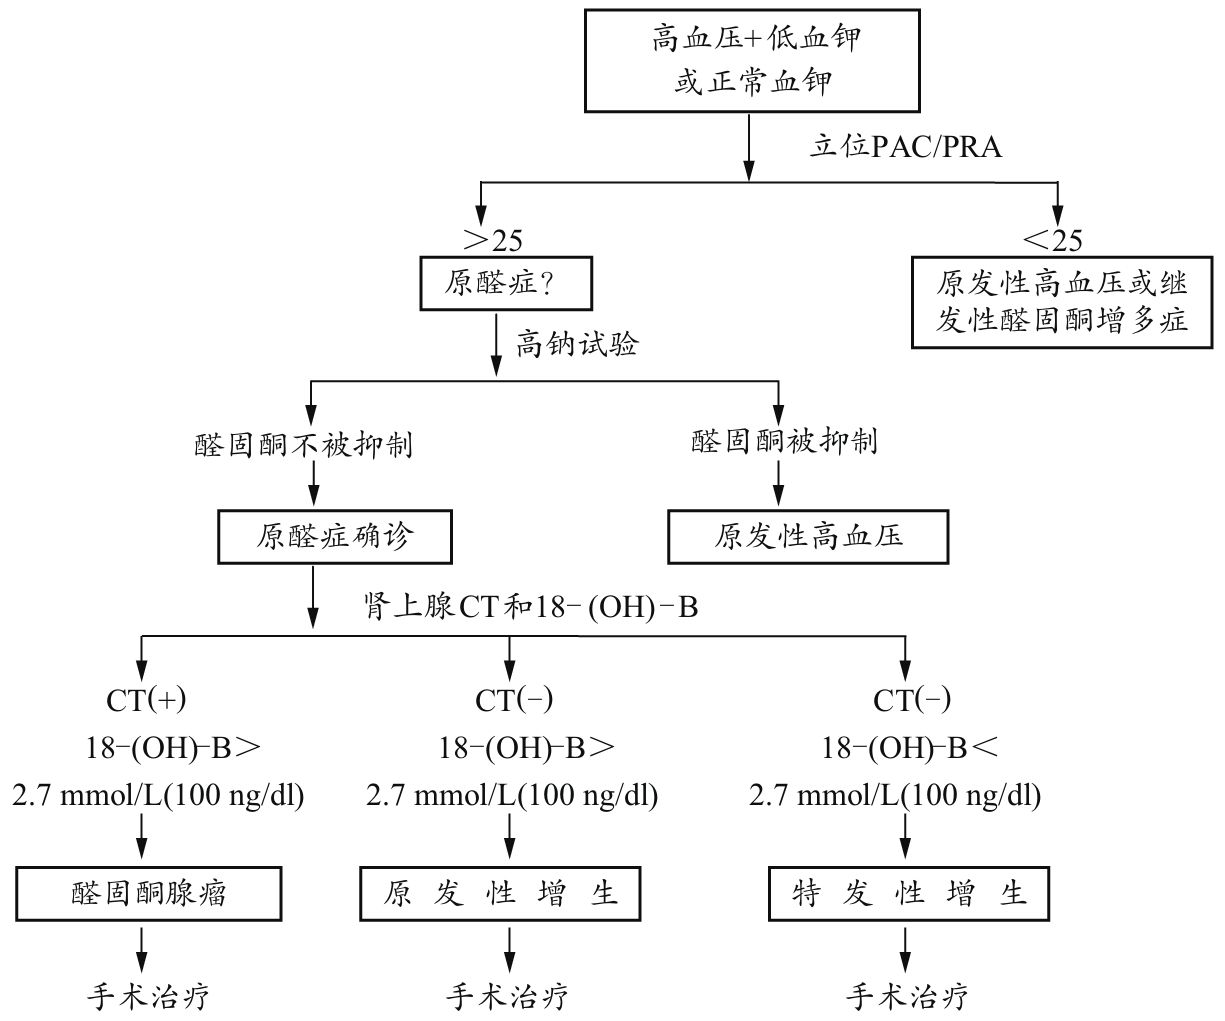
\includegraphics{./images/Image00075.jpg}
 \captionsetup{justification=centering}
 \caption{原发性醛固酮增多症与高血压的治疗程序}
 \label{fig2-7-2}
  \end{figure} 

2.
肾脏疾病与高血压 肾脏疾病包括肾实质病变和肾血管异常,引起的高血压称为肾性高血压,占成人高血压患者的5\%\textasciitilde{}10\%。

(1)肾实质性高血压:病因包括原发性肾小球肾炎、糖尿病性肾病、慢性肾盂肾炎、结缔组织性肾脏疾病、多囊肾、先天性肾发育不全、放射性肾炎、肾结核、肾肿瘤、肾积水、肾移植后等多种肾脏病变引起的高血压。90\%是由于水钠潴留导致的容量依赖性高血压,约10\%为RAAS导致的“肾素依赖型”高血压。对于肾实质性高血压应先处理相应肾实质性疾病,降低血压应包括非药物治疗(即治疗性生活方式改变)和药物治疗,同时应给予其他控制心血管危险因素的药物如他汀、抗血小板等药物。通常需要3种或3种以上降压药联合,将血压控制在130/80mmHg以下,24小时尿蛋白\textgreater{}1g者,血压\textless{}125/75mmHg;联合治疗方案中应包括ACEI、ARB、利尿剂等。

(2)肾血管性高血压:是单侧或双侧肾动脉主干或分支狭窄引起的高血压。常见病因有多发性大动脉炎、肾动脉纤维肌性发育不良和动脉粥样硬化,前两者主要见于青少年(\textless{}40岁),后者见于老年人(\textgreater{}50岁)。通常以一侧或双侧肾动脉及其分支阻塞、狭窄的程度\textgreater{}50\%作为肾动脉狭窄的标准。因肾血流减少,导致肾脏缺血,激活RAAS是其主要发病机制。进展迅速或突然加重的高血压,均应怀疑本症。本症大多有舒张压中、重度升高,在上腹部或背部肋脊角处可闻及血管杂音。肾动脉造影可明确诊断并提供具体狭窄部位,其他检查包括CT肾动脉造影、超声、核素等。治疗可根据患者病情和条件选择经皮肾动脉成形术、手术和药物治疗。肾血管性高血压可选用钙拮抗剂,单侧肾动脉狭窄选用β受体阻滞剂或ACEI或ARB治疗;双侧肾动脉严重狭窄者禁用ACEI或ARB,利尿剂可刺激RAAS系统,对高肾素型肾动脉狭窄不宜选用。

3.
嗜铬细胞瘤与高血压 嗜铬细胞瘤起源于肾上腺髓质、交感神经节和体内其他部位嗜铬组织,肿瘤间歇或持续释放过多肾上腺素、去甲肾上腺素与多巴胺。临床表现多变,典型发作表现为阵发性血压升高伴心动过速、头痛、出汗、面色苍白。发作期间可测定血或尿儿茶酚胺或其代谢产物3-甲氧基-4-羟基苦杏仁酸(VMA),如有显著增高,提示嗜铬细胞瘤。超声、放射性核素、CT或磁共振等可作定位诊断。

嗜铬细胞瘤大多为良性,约10\%嗜铬细胞瘤为恶性,手术切除效果好。术前或恶性病变已有多处转移无法手术者,选择α和β受体阻滞剂联合降压治疗。

4.
皮质醇增多症与高血压 皮质醇增多症又称Cushing综合征,由于促肾上腺皮质激素(ACTH)分泌过多导致肾上腺皮质增生或肾上腺皮质腺瘤,引起糖皮质激素过多所致。80\%患者有高血压,同时合并向心性肥胖、满月脸、水牛背、皮肤紫纹、毛发增多、血糖增高等。24小时尿中17-羟和17-酮类固醇增多,地塞米松抑制试验和肾上腺皮质激素兴奋试验有助于诊断。颅内蝶鞍X线检查,肾上腺CT,放射性核素肾上腺扫描可确定病变部位。治疗主要采用手术、放射和药物方法根治病变本身,降压治疗可采用利尿剂或与其他降压药物联合应用。

5.
主动脉缩窄与高血压 主动脉缩窄多数为先天性,少数为多发性大动脉炎所致。临床表现为上臂血压增高,而下肢血压不高或降低。在肩胛间区、胸骨旁、腋部有侧支循环的动脉搏动和杂音,腹部听诊有血管杂音。胸部X线检查可见肋骨受侧支动脉侵蚀引起的切迹。主动脉造影可确定诊断。治疗包括介入植入支架术或外科手术。

6.
阻塞性睡眠呼吸暂停低通气综合征(OSAS)与高血压 OSAS表现为反复发作的严重打鼾、呼吸暂停、低通气、低氧血症和白天嗜睡。多数患者先有OSAS,逐渐发生高血压;纠正睡眠呼吸暂停低通气后,血压下降或恢复正常。对于OSAS合并高血压患者的降压治疗,选择ACEI、ARB、CCB等,β受体阻滞剂不宜选用,此外可无创持续正压通气治疗、外科治疗,内科治疗还包括减轻体重、侧卧睡眠、戒烟酒、治疗原发病等。

【疗效观察与随访】 针对不同的病因,采取相应的治疗措施,观察治疗后的血压水平以及有无血压增高引起的相应症状。可参阅高血压病等内容。

【治疗经验与解析】

1. 慢性肾脏疾病患者使用利尿剂时应注意

(1)定期监测血压、肾小球滤过率,有无血容量不足及用药后症状性低血压或低GFR。

(2)监测血钾及其他电解质水平。

2.
糖尿病肾病的特点是早期即出现高血压、蛋白尿,同时或继之出现慢性肾脏疾病;原发性高血压肾小球动脉硬化很少出现明显蛋白尿,肾功能减退首先从肾小管浓缩功能开始,逐渐引起血肌酐升高。

3.
并非所有肾动脉狭窄均引起高血压。长期高血压及动脉硬化可引起肾动脉狭窄,原发性高血压与肾血管性高血压并存;缺血性肾病是一种进展性疾病;对肾动脉狭窄的治疗既要考虑血压控制,也要重视对肾功能保护。肾血管性高血压患者血压不宜降压过低,以免导致肾功能严重损害。


\section{心脏瓣膜病}

心脏瓣膜病(valvular heart
disease)是由于炎症、粘液样变性、退行性改变、先天性畸形、缺血性坏死、创伤等原因引起的单个或多瓣膜结构(包括瓣叶、瓣环、腱索或乳头肌)的功能或结构异常,导致瓣口狭窄及(或)关闭不全。心室和主、肺动脉根部严重扩张也可产生相应房室瓣和半月瓣的相对性关闭不全。二尖瓣最常受累,其次为主动脉瓣。

风湿性心脏病(rheumatic heart
disease)简称风心病,指风湿性炎症过程所致的瓣膜损害,主要累及40岁以下人群。我国风心患者群患病率在20世纪70年代成人为1.9‰\textasciitilde{}2.9‰,儿童为0.4‰\textasciitilde{}2.7‰,80年代分别为1.99‰和0.25‰,已有下降。但风心病仍是我国常见的心脏病之一。瓣膜粘液样变性和老年人的瓣膜钙化在我国日益增多。

\subsection{风湿热}

风湿热是常见的风湿性疾病,主要表现为心脏炎、游走性关节炎、舞蹈病、环形红斑和皮下小结,可反复发作。心脏炎是最严重的表现,急性期可危及病儿生命,反复发作可致永久性心脏瓣膜病变,本病好发年龄为6\textasciitilde{}15岁,一年四季均可发病,以冬春多见,是A组乙型溶血性链球菌咽峡炎后的晚期并发症。

【治疗方案】

1. 休息 卧床休息时间取决于心脏受累程度和心功能状态。

(1)急性期无心脏炎患儿:卧床休息2周,随后逐渐恢复活动。

(2)心脏炎无心力衰竭患儿:卧床休息4周,随后于4周内逐渐恢复活动。

(3)心脏炎伴充血性心力衰竭患儿:需卧床休息至少8周,在以后2\textasciitilde{}3个月内逐渐增加活动量。

2.
清除链球菌感染 应用青霉素80万U肌内注射,每日2次,持续2周,青霉素过敏者可改用红霉素等。

3.
抗风湿热治疗 心脏炎时泼尼松每日2mg/kg,最大剂量不超过60mg/d,分次口服,2\textasciitilde{}4周后减量,总疗程8\textasciitilde{}12周。无心脏炎的患儿可用阿司匹林,每日100mg/kg,最大量\textless{}3g/d,分次服用;2周后逐渐减量,疗程4\textasciitilde{}8周。

4.
其他治疗 有充血性心力衰竭给予大剂量静脉注射糖皮质激素,如氢化可的松或甲基泼尼松龙10\textasciitilde{}30mg/kg,每日1次,共1\textasciitilde{}3次;低盐饮食,必要时给予利尿剂如呋塞米20mg,每日1次,安体舒通20mg,每日1次,血管扩张剂如消心痛5mg,每日3次。舞蹈病时用苯巴比妥、安定等。关节肿痛时应予制动。

【疗效观察与随访】

1. 观察指标 临床症状与体征、心电图、血象、血沉、ASO等。

2.
治愈标准 症状、体征消失,3个月未复发,无并发症,相关检查指标恢复正常。

3. 随访 定期复查ASD、BNP、血沉、心电图、心功能及6分钟步行试验等。

【治疗经验与解析】

1.
风湿热预后主要取决于心脏炎的严重程度、首次发作是否得到正确抗风湿热治疗以及是否正规抗链球菌治疗。

2.
每3\textasciitilde{}4周肌内注射卞星青霉素120万U,预防注射期限至少5年,最好持续至25岁,有风湿性心脏病者,宜作终身药物预防,对青霉素过敏者可改用红霉素类药物口服,每月口服6\textasciitilde{}7日,持续时间同前。

3.
风湿热或风湿性心脏病患儿,当拔牙或行其他手术时,术前、术后应用抗生素以预防感染性心内膜炎。

4. 有充血性心力衰竭时,应慎用洋地黄制剂,并注意观察以免发生洋地黄中毒。

\subsection{二尖瓣疾病}

{(一)二尖瓣狭窄}  二尖瓣狭窄(mitral
stenosis)是我国主要的瓣膜病,最常见病因是风湿热,2/3为女性。约半数患者有反复链球菌腭扁桃体炎或咽峡炎史。慢性二尖瓣狭窄导致左心房扩大、钙化,特别合并房颤时左心耳及左心房内易形成附壁血栓。二尖瓣中度狭窄(瓣口面积\textless{}1.5cm{2}
)时,临床逐渐出现症状,主要表现有呼吸困难、咯血、咳嗽、声嘶等;常见体征包括二尖瓣面容,双颧绀红,心尖区有低调的隆隆样舒张中晚期杂音,有时在胸骨左缘第二肋间闻及舒张早期吹风样杂音,称Graham
Steell杂音。并发症有心房颤动、急性肺水肿、血栓栓塞、右心衰竭、感染性心内膜炎、肺部感染等。超声心动图是确诊及量化诊断二尖瓣狭窄的可靠方法。

【治疗程序】 如图\ref{fig2-8-1}所示。

\begin{figure}[!htbp]
 \centering
 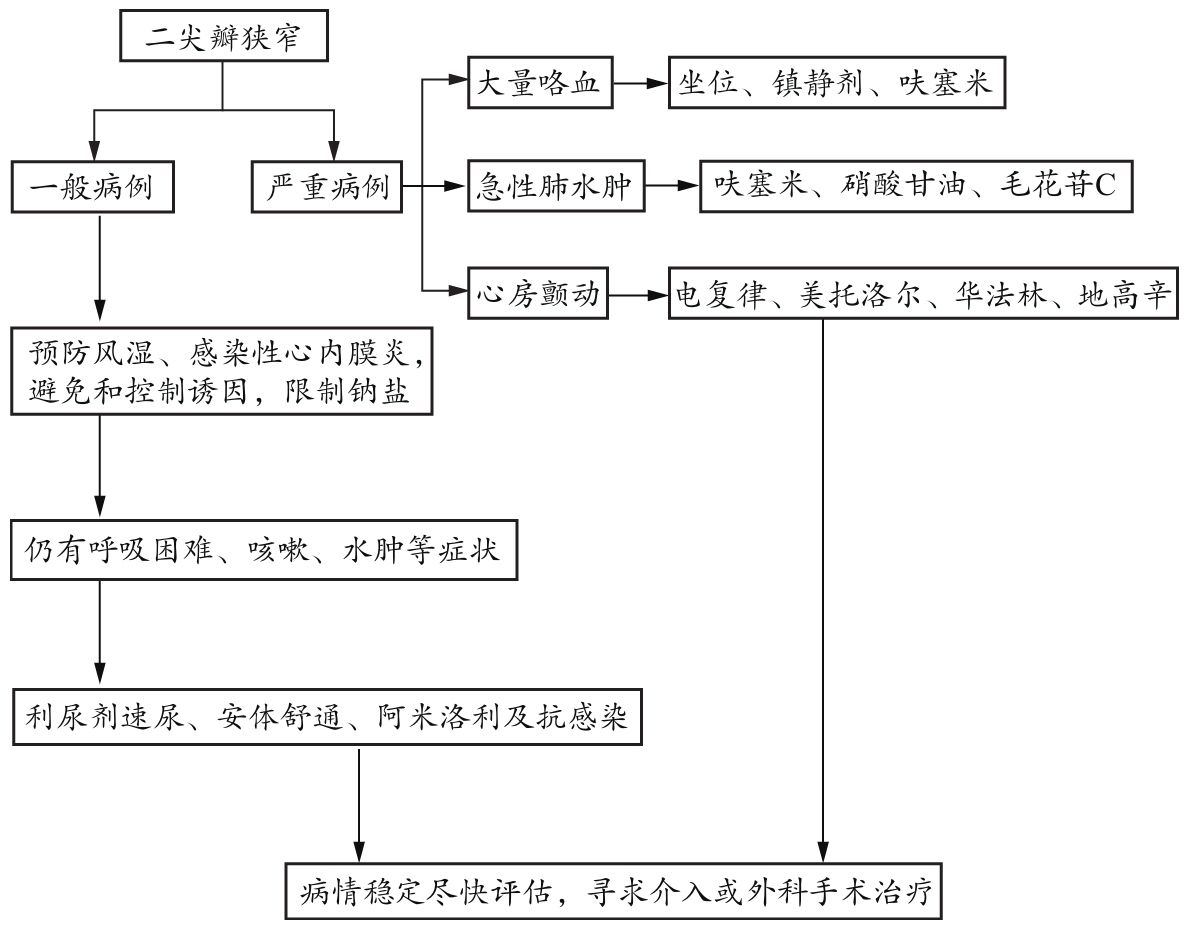
\includegraphics{./images/Image00076.jpg}
 \captionsetup{justification=centering}
 \caption{二尖瓣狭窄的治疗程序}
 \label{fig2-8-1}
  \end{figure} 

【治疗方案】

1. 一般治疗

(1)有风湿活动者应给予抗风湿治疗。特别强调预防风湿热复发,一般应坚持至患者40岁甚至终身应用苄星青霉素120万U,每4周肌内注射1次。

(2)预防感染性心内膜炎:

在口腔、上呼吸道手术或操作,预防药物应针对草绿色链球菌:常用①阿莫西林2.0g,术前1小时口服。②不能口服者,氨苄西林2.0g,术中30分钟内肌内注射或静脉注射。③对青霉素过敏者,克林霉素600mg,术前1小时口服或术前30分钟静脉注射;或头孢氨苄2.0g,术前1小时口服;或头孢唑林1.0g,术前30分钟静脉注射或肌内注射;或头孢羟氨苄2.0g,术前1小时口服;或甲基红霉素500mg,术前1小时口服。高危患者(人工瓣、心内膜炎史、复杂发绀型先天性心脏病或体-肺循环分流术后)术后6小时需重复应用抗生素半量。

泌尿、生殖和消化道手术或操作:预防用药针对肠球菌:①高危患者:予氨苄西林加庆大霉素,即氨苄西林2.0g加庆大霉素1.5mg/kg,术中30分钟内静脉注射或肌内注射,术后6小时,氨苄西林1.0g静脉注射或肌内注射;或阿莫西林1.0g口服。青霉素过敏者予万古霉素加庆大霉素,即万古霉素1.0g,术前30分钟静脉滴注1\textasciitilde{}2小时,加庆大霉素1.5mg/kg,术前30分钟静脉注射或肌内注射。术后不必重复用药。②中危患者(瓣膜病和除外房间隔缺损的先天性心脏病):予阿莫西林或氨苄西林,即阿莫西林2.0g,术前1小时口服;或氨苄西林2.0g,术前30分钟肌内注射或静脉注射。青霉素过敏者予万古霉素,即万古霉素1.0g,术前30分钟静脉滴注1\textasciitilde{}2小时。术后不必重复。

(3)无症状者:避免剧烈体力活动,定期(6\textasciitilde{}12个月)复查。

(4)有呼吸困难者:应减少体力活动,限制钠盐摄入,口服利尿剂,可用呋塞米每日20mg、安体舒通每日20mg口服,避免和控制诱发急性肺水肿的因素,如急性感染、贫血等。

2. 并发症的处理

(1)大量咯血:应取坐位,用镇静剂安定10mg肌内注射,静脉注射呋塞米每次20\textasciitilde{}40mg,以降低肺静脉压。

(2)急性肺水肿:处理原则与急性左心衰竭所致的肺水肿相似。应注意:①避免使用以扩张小动脉为主、减轻心脏后负荷的血管扩张药物,选用扩张静脉系统、减轻心脏前负荷为主的硝酸酯类药物;②正性肌力药物对二尖瓣狭窄的肺水肿无益,仅在心房颤动伴快速心室率时可静脉注射毛花苷C,以减慢心室率。

(3)心房颤动:治疗目的为满意控制心室率,争取恢复和保持窦性心律,预防血栓栓塞。

急性发作伴快速心室率,如血流动力学稳定,可先静脉注射毛花苷C0.2\textasciitilde{}0.4mg,以减慢心室率,该药起效较慢,常不能满意控制心室率,应联合经静脉使用β受体阻滞剂、地尔硫䓬
、维拉帕米;如血流动力学不稳定,出现肺水肿、休克、心绞痛或晕厥时,应立即电复律,如复律失败,尽快用药减慢心室率。

慢性心房颤动:①如心房颤动病程\textless{}1年,左心房直径\textless{}60mm,无高度或完全性房室传导阻滞和病态窦房结综合征,可行电复律或药物转复,成功恢复窦性心律后需长期口服抗心律失常药物,预防或减少复发。复律之前3周和成功复律之后4周需服抗凝药物(华法林),预防栓塞。②如患者不宜复律、或复律失败、或复律后不能维持窦性心律且心室率快,则可口服β受体阻滞剂,控制静息心室率在70次/分左右,日常活动时心率90次/分左右。如心室率控制不满意,可加用地高辛,每日0.125\textasciitilde{}0.25mg。③如无禁忌证,应长期服用华法林,预防血栓栓塞。

(4)预防栓塞:口服华法林,定期监测INR。华法林的初始剂量建议为3mg/d;大于75岁的老年人和出血风险患者,应从2mg开始,每日1次口服,目标INR依病情而定,一般为2.0\textasciitilde{}3.0g。

(5)右心衰竭:限制钠盐摄入,应用利尿剂等。

3.
介入和手术治疗 是治疗本病的有效方法。当二尖瓣口有效面积\textless{}1.5cm{2}
。伴有症状,尤其症状进行性加重时,应用介入或手术方法扩大瓣口面积,减轻狭窄。如肺动脉高压明显,即使症状轻,也应及早干预。

(1)经皮球囊二尖瓣成形术:是缓解单纯二尖瓣狭窄的首选方法。将球囊导管从股静脉经房间隔穿刺跨越二尖瓣,用生理盐水和造影剂各半的混合液体充盈球囊,分离瓣膜交界处的粘连融合而扩大瓣口。在瓣叶(尤其是前叶)活动度好,无明显钙化,瓣下结构无明显增厚者效果较好。高龄、伴有严重冠心病,因其他严重的肺、肾、肿瘤等疾病不宜手术或拒绝手术、妊娠伴严重呼吸困难、外科分离术后再狭窄患者也可选择该疗法。术前用食管超声探查有无左心房血栓,对有血栓或慢性心房颤动患者应在术前充分用华法林抗凝。术后症状和血流动力学立即改善,严重并发症少见,主要应注意减少二尖瓣关闭不全、脑栓塞和心房穿孔所致的心脏压塞,手术死亡率\textless{}0.5\%。其近期与远期(5年)效果与外科闭式分离术相似,基本可取代后者。

(2)闭式分离术:经开胸手术,将扩张器由左心室心尖部插入二尖瓣口分离瓣膜交界处的粘连融合,适应证和效果与经皮球囊二尖瓣成形术相似,目前临床已很少使用。

(3)直视分离术:适用于瓣叶严重钙化、病变累及腱索和乳头肌、左心房内有血栓的二尖瓣狭窄的患者。在体外循环下,直视分离融合的交界处、腱索和乳头肌,去除瓣叶的钙化斑,清除左心房内血栓。较闭式分离术解除瓣口狭窄程度大,因而血流动力学改善更好。手术死亡率\textless{}2\%。

(4)人工瓣膜置换术适应证为:①严重瓣叶和瓣下结构钙化、畸形,不宜做分离术者;②二尖瓣狭窄合并明显二尖瓣关闭不全者。手术应在有症状而无严重肺动脉高压时考虑。严重肺动脉高压增加手术风险,并非手术禁忌,术后多有肺动脉高压减轻。人工瓣膜置换术手术死亡率(3\%\textasciitilde{}8\%)和术后并发症均高于分离术。术后存活者,心功能恢复较好。

【疗效观察与随访】

1. 观察指标 相关症状、体征、心功能、6分钟步行试验、UCG、BNP等。

2. 临床疗效判定

显效:术后症状、体征消失,心功能恢复至正常范围,UCG、BNP显著改善。

好转:临床症状、NYHA心功能分级、6分钟步行试验等有一定程度改善。

3. 随访 术后定期监测症状、体征及心功能变化。

【治疗经验与解析】 在未开展手术治疗的年代,在无症状被确诊后,本病10年存活率84\%,症状轻者为42\%,中、重度者为15\%。从发生症状到完全致残期平均7.3年。死亡原因为心力衰竭(62\%)、血栓栓塞(22\%)和感染性心内膜炎(8\%)。抗凝治疗后,栓塞发生减少。手术治疗提高了患者的生活质量和存活率,如有条件应尽早进行。

{(二)二尖瓣关闭不全}
 收缩期二尖瓣关闭依赖二尖瓣装置如瓣叶、瓣环、腱索、乳头肌等,及左心室的结构、功能的完整性,其中任何部分异常可致二尖瓣关闭不全(mitral
incompetence)。常见病因有风湿性损害、原发性粘液性变、感染性心内膜炎、肥厚型心肌病、急性心肌梗死、退行性变等。临床表现有急性左心衰竭,严重时发生急性肺水肿、心源性休克;慢性发作导致心排出量减少,常见症状如疲乏、无力,肺淤血症状如呼吸困难出现较晚。心脏听诊为全收缩期吹风样高调杂音,在心尖区最响。杂音向左腋下和左肩胛下区传导。冠心病乳头肌功能失常时可有收缩早期、中期、晚期或全收缩期杂音。腱索断裂时杂音可似海鸥鸣或乐音性。脉冲式多普勒超声和彩色多普勒血流显像诊断二尖瓣关闭不全的敏感性近100\%。并发症包括心房颤动、感染性心内膜炎、脑栓塞、心律失常、猝死、腱索断裂、严重二尖瓣关闭不全和心力衰竭。

【治疗方案】

1.
急性二尖瓣关闭不全 治疗目的是降低肺静脉压,增加心排出量和纠正病因。内科治疗一般为术前过渡措施,尽可能在床旁Swan-Ganz导管血流动力学监测指导下进行。静脉滴注硝普钠通过扩张小动静脉,降低心脏前、后负荷,减轻肺淤血,减少反流,增加心排出量。静脉注射利尿剂有助于降低前负荷。外科治疗为根本措施,视病因、病变性质、反流程度和对药物治疗的反应,采取紧急、择期或选择性手术(人工瓣膜置换术或修复术)。部分患者经药物治疗后症状基本控制,进入慢性代偿期。

2. 慢性二尖瓣关闭不全

(1)内科治疗:①风心病伴风湿活动者,需抗风湿治疗并预防风湿热复发。②预防感染性心内膜炎。③无症状、心功能正常者无需特殊治疗,但应定期随访。④心房颤动的处理同二尖瓣狭窄,但维持窦性心律不如在二尖瓣狭窄时重要。除因心房颤动导致心功能显著恶化需恢复窦性心律外,多数只需满意控制心室率。慢性心房颤动,有体循环栓塞史、超声检查见左心房血栓者,应长期抗凝治疗。⑤心力衰竭者应限制钠盐摄入,使用利尿剂、血管紧张素转换酶抑制剂、β受体阻滞剂和洋地黄。

(2)外科治疗:为恢复瓣膜关闭完整性的根本措施。应在发生不可逆的左心室功能不全之前施行,否则术后预后不佳。慢性二尖瓣关闭不全的手术适应证:①重度二尖瓣关闭不全伴心功能NYHAⅢ或Ⅳ级;②心功能NYHAⅡ级伴心脏大,左室收缩末期容量指数(LVESVI)\textgreater{}30ml/m{2}
;③重度二尖瓣关闭不全,左室射血分数(LVEF)减低,左室收缩及舒张末期内径增大,LVESVI高达60ml/m{2}
,虽无症状也应考虑手术治疗。严重二尖瓣关闭不全,术前LVESVI正常(\textless{}30ml/m{2}
)的患者,术后左室功能正常;而LVESVI显著增加者(\textgreater{}90ml/m{2}
),围术期死亡率增加,术后心功能差;LVESVI中度增加者(30\textasciitilde{}90ml/m{2}
)常能耐受手术,术后心功能可能减低。手术方法有瓣膜修补术和人工瓣膜置换术二种:

瓣膜修补术:如瓣膜损坏较轻,瓣叶无钙化,瓣环有扩大,腱索无严重增厚者可行瓣膜修复成形术。瓣膜修复术死亡率低,能获得长期临床改善,作用持久。术后发生感染性心内膜炎和血栓栓塞少,不需长期抗凝,左心室功能恢复较好。手术死亡率为1\%\textasciitilde{}2\%。与换瓣相比,较早和较晚期均可考虑瓣膜修补手术,但LVEF≤0.15\textasciitilde{}0.20时为禁忌。

人工瓣膜置换术:瓣叶钙化,瓣下结构病变严重,感染性心内膜炎或合并二尖瓣狭窄者必须置换人工瓣。感染性心内膜炎感染控制不满意或反复栓塞或合并心衰药物治疗不满意者提倡早做换瓣手术,真菌性心内膜炎应在心衰或栓塞发生之前行换瓣手术。目前换瓣手术死亡率约5\%左右。多数患者术后症状和生活质量改善,肺动脉高压减轻,心脏大小和左心室重量减少,较内科治疗存活率明显改善,但心功能改善不如二尖瓣和主动脉瓣置换术满意。严重左心室功能不全(LVEF≤0.30\textasciitilde{}0.35)或左心室重度扩张(左心室舒张末内径LVEDα≥80mm,左心室舒张末容量指数LVEDVI≥300ml/m{2}
),不宜换瓣。

【疗效观察与随访】

1. 观察指标 症状、体征、心功能、6分钟步行试验、UCG、BNP等。

2.
临床疗效判定 显效:症状、体征消失,心功能改善,6分钟步行试验等明显改善,UCG、BNP明显改善。

3.
随访 术后1年内定期观察临床症状和体征的变化,必要时复查心功能、UCG、BNP等。

【治疗经验与解析】 急性严重反流伴血流动力学不稳定者,如不及时手术干预,死亡率极高。在手术治疗前的年代,慢性重度二尖瓣关闭不全确诊后内科治疗5年存活率80\%,10年存活率60\%。单纯二尖瓣脱垂无明显反流,无收缩期杂音者大多预后良好;年龄\textgreater{}50岁、有明显收缩期杂音和二尖瓣反流、瓣叶冗长增厚、左心房左心室增大者预后较差。

\subsection{主动脉瓣疾病}

{(一)主动脉瓣狭窄}
 主动脉瓣狭窄常见病因有:风心病、先天性畸形、老年退化性主动脉瓣狭窄。常见临床表现有呼吸困难、心绞痛和晕厥。心脏听诊可闻及收缩期喷射性杂音,在第一心音稍后或紧随喷射音开始,止于第二心音前,为吹风样、粗糙、递增递减型,在胸骨右缘第2或左缘第3肋间最响,主要向颈动脉、也可向胸骨左下缘传导,常伴震颤。有细迟脉。超声心动图是明确诊断和判定狭窄程度的重要方法。并发症有心房颤动、室性心律失常、心脏性猝死、感染性心内膜炎、体循环栓塞、心力衰竭、胃肠道出血等。

【治疗方案】

1.
内科治疗 主要目的为确定狭窄程度,观察狭窄进展情况,为有手术指征患者选择合理手术时间。

(1)预防感染性心内膜炎:风心病伴风湿活动者,应预防风湿热。

(2)无症状的轻度狭窄患者:每2年复查1次,包括超声心动图定量测定。中和重度狭窄患者:避免剧烈体力活动,每6\textasciitilde{}12个月复查1次。

(3)合并频发房性期前收缩:应予抗心律失常药物,如胺碘酮0.2,每日1次,预防心房颤动。

(4)心绞痛:可试用硝酸酯类药物如硝酸异山梨酯10mg,每日3次。

(5)心力衰竭者:应限制钠盐摄入,可用洋地黄类药物如地高辛0.125mg,每日1次;应用利尿剂,如双氢克尿噻25mg、每日1次,呋噻米20\textasciitilde{}40mg,每日1次。

2.
外科治疗 人工瓣膜置换术为治疗成人主动脉狭窄的主要方法。无症状的轻、中度狭窄患者无手术指征。重度狭窄(瓣口面积\textless{}0.75cm{2}
或平均跨瓣压差\textgreater{}50mmHg)伴心绞痛、晕厥或心力衰竭症状为手术的主要指征。无症状的重度狭窄患者,如伴有进行性心脏增大和(或)明显左心室功能不全,也应考虑手术。严重左心室功能不全、高龄、合并主动脉瓣关闭不全或冠心病,增加手术和术后晚期死亡风险,但不是手术禁忌证。手术死亡率≤5\%。有冠心病者,需同时作冠状动脉旁路移植术。术后的远期预后优于二尖瓣疾病和主动脉关闭不全的换瓣患者。

儿童和青少年的非钙化性先天性主动脉瓣严重狭窄,甚至包括无症状者,可在直视下行瓣膜交界处分离术。

3.
经皮球囊主动脉瓣成形术 经股动脉逆行将球囊导管推送至主动脉瓣,用生理盐水与造影剂各半的混合液体充盈球囊,裂解钙化结节,伸展主动脉瓣环和瓣叶,解除瓣叶和分离融合交界处,减轻狭窄和症状。近年,也发展了经皮主动脉瓣膜置换术,疗效待观察。

尽管此技术的中期结果令人失望(操作死亡率3\%,1年死亡率45\%),但它主要的治疗对象为高龄、有心力衰竭和手术高危患者,在不适于手术治疗的严重钙化性主动脉瓣狭窄患者仍可改善左心室功能和症状,适应证包括:①严重主动脉瓣狭窄的心源性休克者;②严重主动脉瓣狭窄需急诊非心脏手术治疗,因有心力衰竭而具极高手术危险者,作为以后人工瓣膜置换的过渡;③严重主动脉狭窄的妊娠妇女,无法保证胎儿生存者;④严重主动脉瓣狭窄,拒绝手术治疗的患者。

与经皮球囊二尖瓣成形不同,经皮球囊主动脉瓣成形的临床应用范围局限。

【疗效观察与随访】 参见二尖瓣狭窄章节。

【治疗经验与解析】

1.
主动脉狭窄患者不能耐受心房颤动,一旦出现,应及时转复为窦性心律。其他可导致症状或血流动力学后果的心律失常也应积极治疗。

2.
伴有心力衰竭者应小心应用利尿剂,过度利尿可因低血容量致左心室舒张末压降低和心排血量减少,发生直立性低血压。不宜使用小动脉血管扩张剂,以防血压过低。

3.
可多年无症状,但大部分患者的狭窄进行性加重,一旦出现症状,预后恶化,出现症状后的平均寿命仅3年左右,其中,出现晕厥后为3年、心绞痛为5年、左心衰竭\textless{}2年。死亡原因为左心衰竭(70\%)、猝死(15\%)和感染性心内膜炎(5\%)。退行性钙化性狭窄较先天性或风湿性病变发展迅速。未手术治疗的症状性患者预后较二尖瓣疾病或主动脉瓣关闭不全患者差。人工瓣膜置换术后预后明显改善,手术存活者的生活质量和远期存活率显著优于内科治疗的患者。

{(二)主动脉瓣关闭不全}
 主动脉瓣关闭不全是由于主动脉瓣及(或)主动脉根部疾病所致。急性病变病因包括感染性心内膜炎、创伤、主动脉夹层、人工瓣撕裂。慢性病变病因有:主动脉瓣疾病如风心病、感染性心内膜炎、先天性畸形、主动脉瓣粘液样变性、强直性脊柱炎,主动脉根部扩张如梅毒性主动脉炎、Marfan综合征、强直性脊柱炎、升主动脉瘤等。临床表现:急性病变如急性左心衰竭和低血压。慢性病变如心悸、心前区不适、头部强烈搏动感等症状,晚期始出现左心室衰竭表现。常见体征为与第二心音同时开始的高调叹气样递减型舒张早期杂音,坐立前倾位和深呼气时易听到,杂音在胸骨左中下缘明显;重度反流者,常在心尖区听到舒张中晚期隆隆样杂音(Austin-Flint杂音)。超声心动图为明确诊断和判定关闭不全程度的重要方法。并发症:感染性心内膜炎较常见;可发生室性心律失常但心脏性猝死少见;心力衰竭在急性者出现早,慢性者于晚期始出现。

【治疗方案】

1.
急性主动脉瓣关闭不全 外科治疗(人工瓣膜置换术或主动脉瓣修复术)为根本措施。内科治疗一般仅为术前准备过渡措施,目的在于降低肺静脉压,增加心排出量,稳定血流动力学,应尽量在Swan-Granz导管床旁血流动力学监测下进行。静脉滴注硝普钠有助于降低前后负荷、改善肺淤血、减少反流量和增加排血量。也可酌情经静脉使用利尿剂和正性肌力药物。血流动力学不稳定者,如严重肺水肿,应立即手术。主动脉夹层即使伴轻或中度反流,也需紧急手术。活动性感染性心内膜炎患者,争取在完成7\textasciitilde{}10日强化抗生素治疗后手术。创伤性或人工瓣膜功能障碍者,根据病情采取紧急或择期手术。个别患者药物可完全控制病情,心功能代偿良好,手术可延缓。但真菌性心内膜炎所致者,无论反流轻重,几乎均需早日手术。

2. 慢性主动脉瓣关闭不全

(1)内科治疗:适用于①预防感染性心内膜炎,风心病患者伴风湿活动应预防风湿热。②梅毒性主动脉炎,应予青霉素治疗。③舒张压\textgreater{}90mmHg者应用降压药。④无症状的轻或中度反流者,应限制重体力活动,并每1\textasciitilde{}2年随访1次,应包括超声心动图检查。在有严重主动脉瓣关闭不全和左心室扩张者,即使无症状,也可使用血管紧张素转换酶抑制剂,以延长无症状和心功能正常时期,推迟手术时间。⑤左室收缩功能不全出现心力衰竭时应用血管紧张素转换酶抑制剂和利尿剂,必要时可加用洋地黄类药物。⑥心绞痛可用硝酸酯类药物。⑦积极纠正心房颤动和治疗心律失常,主动脉瓣关闭不全患者耐受这些心律失常的能力极差。⑧如有感染应及早积极控制。

(2)外科治疗:人工瓣膜置换术为严重主动脉瓣关闭不全的主要治疗方法,应在不可逆性左心室功能不全发生之前进行,注意掌握手术时机。无症状(呼吸困难或心绞痛)和左心室功能正常的严重反流不需手术,但需密切随访。下列情况的严重关闭不全应手术治疗:①有症状和左心室功能不全者;②无症状伴左心室功能不全者,经系列无创检查(超声心动图、放射性核素心室造影等)显示持续或进行性左心室收缩末容量增加或静息射血分数降低者应手术;如左心室功能测定为临界值或不恒定的异常,应密切随访;③有症状而左心室功能正常者,先试用内科治疗,如无改善,不宜拖延手术时间。手术的禁忌证为LVEF≤0.15\textasciitilde{}0.20,LVEDD≥80mm或LVEDVI≥300ml/m{2}
。术后存活者大部分有明显临床改善,心脏大小和左心室重量减少,左心室功能有所恢复,但恢复程度不如主动脉瓣狭窄者大,术后远期存活率也低于后者。部分病例(如创伤、感染性心内膜炎所致瓣叶穿孔)可行瓣膜修复术。主动脉根部扩大者,如Marfan综合征,需行主动脉根部带瓣人工血管移植术。

【疗效观察与随访】 参见二尖瓣狭窄章节。

【治疗经验与解析】 急性重度主动脉瓣关闭不全如不及时手术治疗,常死于左心室衰竭。慢性者无症状期长。重度者经确诊后内科治疗5年存活率为75\%,10年存活率50\%。症状出现后,病情迅速恶化,心绞痛者5年内死亡50\%,严重左心室衰竭者2年内死亡50\%。

\subsection{三尖瓣疾病}

{(一)三尖瓣狭窄}  三尖瓣狭窄(tricuspid
stenosis)最常见病因为风心病,单独存在者极少见,常伴关闭不全、二尖瓣和主动脉瓣损害。女性多见,其他罕见病因有先天性三尖瓣闭锁和类癌综合征等。临床表现为心排出量低引起疲乏,体循环淤血致腹胀。可并发心房颤动和肺栓塞。体征:颈静脉扩张、胸骨左下缘有三尖瓣开瓣音、胸骨左缘第4、5肋间或剑突附近有紧随开瓣音后的,较二尖瓣狭窄杂音弱而短的舒张期隆隆样杂音,伴舒张期震颤。杂音和开瓣音均在吸气时增强,呼气时减弱、肝大伴收缩期前搏动、腹水和全身水肿。超声心动图确诊三尖瓣狭窄具有高度敏感性和特异性。

【治疗方案】

1. 内科治疗 限制钠盐摄入,应用利尿剂,控制心房颤动的心室率。

2.
外科治疗 跨三尖瓣压差\textgreater{}5mmHg或瓣口面积\textless{}2.0cm{2}
时,应手术治疗。风心病可作瓣膜交界分离术或人工瓣膜置换术。三尖瓣置换术死亡率2\textasciitilde{}3倍于二尖瓣或主动脉瓣置换术。

3. 经皮球囊三尖瓣成形术 虽易行,但适应证尚不明确。

【疗效观察与随访】 参见二尖瓣狭窄章节。

【治疗经验与解析】 本病应查明病因,针对病因治疗。手术治疗应慎重选择手术方式,经皮球囊三尖瓣成形术尚在探索中。

{(二)三尖瓣关闭不全}  三尖瓣关闭不全(tricuspid
incompetence)远较狭窄多见。功能性三尖瓣关闭不全常见,多见于风湿性二尖瓣病、先天性心血管病(肺动脉瓣狭窄、艾森门格综合征)和肺心病等;器质性三尖瓣关闭不全较少见,包括三尖瓣下移畸形(Ebstein畸形)、风心病、三尖瓣脱垂、感染性心内膜炎、冠心病、类癌综合征、心内膜心肌纤维化等。临床表现重者有疲乏、腹胀等右心室衰竭症状。三尖瓣关闭不全的杂音为高调、吹风样和全收缩期,在胸骨左下缘或剑突区最响,右心室显著扩大占据心尖区时,在心尖区最明显。杂音随吸气增强,当右心室衰竭,心搏量不能进一步增加时,此现象消失。并发症有心房颤动和肺栓塞。超声心动图为明确诊断和判定关闭不全程度的重要方法。

【治疗方案】

1.
内科治疗 右心衰竭者,限制钠盐摄入,加用利尿剂、洋地黄类药物和血管扩张药,控制心房颤动的心室率。

2.
外科治疗 继发于二尖瓣或主动脉瓣疾病者,在行人工瓣膜置换术前,评估三尖瓣反流程度,轻者不需手术,中度反流可行瓣环成形术,重者行瓣环成形术或人工瓣膜置换术。三尖瓣下移畸形、类癌综合征、感染性心内膜炎等需作人工瓣膜置换术。

【疗效观察与随访】 参见二尖瓣狭窄章节。

【治疗经验与解析】

1.
单纯三尖瓣关闭不全而无肺动脉高压,如继发于感染性心内膜炎或创伤者,一般不需要手术治疗。中、重度者可行瓣环成形术。重度者尚可行人工瓣膜置换术。

2. 本病应密切观察可能出现的并发症,特别是肺栓塞。

3.
积极治疗其他原因引起的心力衰竭,可改善功能性三尖瓣反流的严重程度。二尖瓣病变伴肺动脉高压及右心室显著扩大时,纠正二尖瓣异常,降低肺动脉压后,三尖瓣关闭不全可逐渐减轻或消失而不必特别处理。

\subsection{肺动脉瓣疾病}

{(一)肺动脉瓣狭窄}  肺动脉瓣狭窄(pulmonary
stenosis)的最常见病因为先天性畸形,风湿性极少见,且极少严重者,总是合并其他瓣膜损害,临床表现为后者掩盖。先天性肺动脉瓣狭窄(congenital
pulmonary valve
stenosis)指肺动脉瓣、瓣上或瓣下有狭窄。此种先天性畸形常单独出现,发病率较高,特别在成人先天性心脏病中可达25\%。轻症肺动脉瓣狭窄可无症状,重者在活动时有呼吸困难及疲倦,严重狭窄者可因剧烈活动而导致晕厥甚至猝死。典型的体征为胸骨左缘第二肋有一响亮的收缩期喷射性杂音,传导广泛可传及颈部,整个心前区甚至背部,常伴有震颤;肺动脉区第二心音减弱。X线检查、超声心动图检查有助于诊断。应用多普勒技术可计算出跨瓣或狭窄上下压力阶差。介入或手术治疗前应行右心导管检查及右心室造影以确定狭窄部位及程度。

【治疗方案】

1.
内科治疗 主要目的确定狭窄程度,观察狭窄进展情况,为有手术指征的患者选择合理手术时间。①无症状的轻度狭窄患者:每2年复查1次,包括超声心动图定量测定。中、重度狭窄患者应避免剧烈体力活动,每6\textasciitilde{}12个月复查1次。②频发房性期前收缩时,应予抗心律失常药物,预防心房颤动,如胺碘酮0.2,每日1次。③心力衰竭者应限制钠盐摄入,可用洋地黄类药物如地高辛0.125mg,每日1次;小心应用利尿剂,如双氢克尿噻25mg,每日1次。

2. 介入治疗 经皮球囊肺动脉瓣成形术(percutaneous balloon pulmonary
valvuloplasty,PBPV)

(1)适应证:①以单纯肺动脉瓣狭窄伴有狭窄后扩张者效果最佳。②狭窄程度以跨瓣压差为标准,过去以≥50mmHg为介入指征,由于技术进展,手术安全性提高,目前趋向于将介入指征降为≥30mmHg。③肺动脉瓣狭窄,经手术治疗后出现再狭窄者亦可进行PBPV。④作为复杂性先天性心脏病的姑息治疗,如室间隔完整型肺动脉闭锁等。⑤肺动脉瓣狭窄并其他可介入治疗的先心病如ASD、PDA等。

(2)禁忌证:①肺动脉瓣下狭窄即右室流出道漏斗部狭窄者。②肺动脉瓣上型狭窄瓣膜发育不良,无肺动脉狭窄后扩张者。

(3)并发症:主要为穿刺部位血管并发症,术中心律失常,三尖瓣受损及继发性肺动脉瓣关闭不全。此类并发症多与术者的经验,操作技术水平有关。

3.
外科治疗 球囊扩张不成功或不宜行球囊扩张者,如狭窄上下压力阶差\textgreater{}40mmHg应采取手术治疗。

【疗效观察与随访】 参见二尖瓣狭窄章节。

【治疗经验与解析】 轻度狭窄一般可不予治疗,随访观察即可。如患者有症状压力阶差\textgreater{}35mmHg者,介入或手术治疗效果均良好;PBPV治疗如适应证选择适当,近期及远期疗效与手术治疗相同,术后压力阶差明显下降者达75\%,但并发症及死亡率明显低于手术治疗,并发症\textless{}6\%,总死亡率\textless{}0.5\%。重症狭窄如不予处理,可致右心衰竭而死亡。

{(二)肺动脉瓣关闭不全}
 最常见病因为继发于肺动脉高压的肺动脉干根部扩张,引起瓣环扩大,见于风湿性二尖瓣疾病、艾森曼格综合征等情况。少见病因包括特发性和Marfan综合征的肺动脉扩张。肺动脉瓣关闭不全(pulmonary
incompetence)导致右心室容量负荷过度。如无肺动脉高压,可多年无症状;如有肺动脉高压,则加速右心室衰竭发生。多数病例因原发病的临床表现突出,肺动脉瓣关闭不全的表现被掩盖,仅偶然于听诊时发现。继发于肺动脉高压者,在胸骨左缘第2\textasciitilde{}4肋间有第二心音后立即开始的舒张早期叹气样高调递减型杂音,吸气时增强,称为Graham
Steell杂音。由于肺动脉扩张和右心搏量增加,在胸骨左缘第2肋间在喷射音后有收缩期喷射性杂音。多普勒超声对确诊肺动脉瓣关闭不全极为敏感,可半定量反流程度。二维超声心动图有助于明确病因。

【治疗方案】 以治疗导致肺动脉高压的原发性疾病为主,如缓解二尖瓣狭窄。仅在严重的肺动脉瓣反流导致难治性右心衰竭时,方考虑对该瓣膜进行手术治疗。

【疗效观察与随访】 参见二尖瓣狭窄章节。

【治疗经验与解析】 病因治疗后仍存在难治性右心衰竭,在无禁忌证的情况下,应尽早行手术治疗。三尖瓣中度反流可作瓣环成形术,重度者行瓣环成形术或瓣膜置换术,Ebstein畸形应行人工瓣膜成形术。

\subsection{多瓣膜病}

多瓣膜病(multivalvular heart
disease)的病因包括:一种疾病同时损害几个瓣膜、一个瓣膜损害致心脏容量或压力负荷过度相继引起近端瓣膜功能受累、不同疾病分别导致不同瓣膜损害。常见多瓣膜病:二尖瓣狭窄伴主动脉瓣关闭不全、二尖瓣狭窄伴主动脉瓣狭窄、主动脉瓣狭窄伴二尖瓣关闭不全、主动脉瓣关闭不全伴二尖瓣关闭不全、二尖瓣狭窄伴三尖瓣和(或)肺动脉瓣关闭不全。

【治疗方案】 内科治疗同单瓣膜损害者。手术治疗为主要措施。

【疗效观察与随访】 参见二尖瓣狭窄章节。

【治疗经验与解析】 多瓣膜人工瓣膜置换术死亡危险高,预后不良,术前确诊和明确相对严重程度对治疗决策至关重要。例如严重二尖瓣狭窄可掩盖并存的主动脉瓣疾病,如果手术仅纠正前者,将致左心室负荷剧增,引起急性肺水肿,增加手术死亡率。左心人工瓣膜置换术时,对明显受累的三尖瓣未作相应手术,术后临床改善不佳。继发于主动脉瓣关闭不全的二尖瓣关闭不全,轻者于主动脉瓣置换术后可缓解,较重者需作瓣环成形术。因此,术前应用左、右心导管检查和心血管造影以确定诊断。有些情况,如三尖瓣损害在手术中方可确诊。


\section{先天性心脏病}

\subsection{无分流的先天性心脏病}

{(一)先天性肺动脉瓣狭窄}  先天性肺动脉瓣狭窄(congenital pulmonary
valve
stenosis)指肺动脉瓣、瓣上或瓣下有狭窄。此种先天性畸形常单独出现,发病率较高,特别在成人先天性心脏病中达25\%。可分为三型:瓣膜型、瓣下型和瓣上型。主要病理生理为右心室排血受阻,右室压力增高,右室代偿性肥厚,最终右室扩大导致衰竭。根据右室压力高低判断病情轻重,如右室收缩压\textless{}50mmHg为轻型;\textgreater{}50mmHg但未超过左室收缩压者为中型;超过左室收缩压者为重型。右室压力越高表明肺动脉瓣狭窄越重,而狭窄处压力阶差越大。轻症肺动脉瓣狭窄可无症状,重者在活动时有呼吸困难及疲倦,严重狭窄者可因剧烈活动而导致晕厥甚至猝死。典型的体征为胸骨左缘第2肋有一响亮的收缩期喷射性杂音,传导广泛可传及颈部,整个心前区甚至背部,常伴有震颤;肺动脉区第二心音减弱。

【治疗方案】

1. 内科治疗 以控制心衰症状,对症处理为主。

2. 球囊扩张术

(1)适应证:①典型主动脉瓣狭窄,心输出量正常时经导管检查跨主动脉瓣压差≥50mmHg,无或仅轻度主动脉瓣反流。由于技术的进展,手术安全性提高,目前已趋向于将介入指征降为≥30mmHg。②肺动脉瓣狭窄,经手术治疗后出现再狭窄者亦可进行PBPV。③作为复杂性先天性心脏病的姑息治疗,如室间隔完整型肺动脉闭锁等。④肺动脉瓣狭窄并其他可介入治疗的先心病如ASD、PDA等。

(2)禁忌证:①主动脉瓣狭窄伴中度以上主动脉瓣反流。②发育不良型主动脉瓣狭窄。③纤维肌性或管道样主动脉瓣下狭窄。④单纯主动脉瓣上狭窄。

3.
手术治疗 球囊扩张不成功或不宜行球囊扩张者,如狭窄上下压力阶差\textgreater{}40mmHg应采取手术治疗。

【疗效观察与随访】

1. 观察指标 临床症状、体征、心电图、超声心动图、X线胸片等。

2.
疗效观察 符合以下条件为效果良好:①未发生或加重主动脉瓣反流。②跨主动脉瓣压差下降50\%以上。③主动脉瓣口面积增大25\%以上。

3.
随访 ①术后2小时内及24小时复查超声心动图。②术后1、3、6及12个月随访,包括临床检查、心电图、X线胸片及超声心动图。

【治疗经验与解析】

1.
为避免股静脉损伤,对无症状非紫绀患儿,可在2\textasciitilde{}4岁行肺动脉瓣膜成形术。

2.
一般选择球囊要大于瓣环径的20\%\textasciitilde{}40\%。为安全起见,重症PS可先选用较小球囊扩张,使严重PS得到初步改善,随后再以足够大的球囊进行扩张。还可选用双球囊扩张。

3.
球囊扩张术后伴右室流出道反应性狭窄者,给予β受体阻滞剂口服,通常维持3\textasciitilde{}6月。

{(二)先天性主动脉缩窄}  先天性主动脉缩窄(congenital coarctation of
the
aorta)为局限性主动脉管腔狭窄,常伴有明显症状及体征,多于婴幼儿期即被发现,大多存活至成年。在成人先天性心脏病中所占比例较小,根据首都医科大学附属北京安贞医院统计仅为0.35\%。有50\%以上合并无明显血流动力学障碍的二叶主动脉瓣畸形,临床表现为血压增高,可导致头痛、头晕、面部潮红、鼻出血等;缩窄以下供血不足而有下肢无力、麻木、发凉甚至有间歇性跛行。心尖搏动增强,心界常向左下扩大,沿胸骨左缘到中上腹可闻及收缩中后期喷射性杂音,有时可在左侧背部闻及。

【治疗方案】

1. 内科治疗 主要是改善心功能及对症治疗。

2. 球囊扩张术

(1)适应证:①主动脉缩窄外科手术后再狭窄,经导管测压静态跨缩窄段收缩压差\textgreater{}20mmHg。②未经外科手术的局限性、隔膜型主动脉缩窄,通常年龄\textgreater{}7个月,压力标准同上。

(2)非适应证:峡部发育不良或长段型主动脉缩窄。

3.
外科手术治疗 适应证包括峡部发育不良、长段型主动脉缩窄和球囊扩张术失败的患者。

【疗效观察与随访】

1. 观察指标 临床症状、体征、心电图、超声心动图、X线胸片,必要时作MRI。

2.
疗效观察 符合以下条件为效果良好:①跨缩窄段压差≤20mmHg。②球囊扩张后主动脉缩窄段直径较术前扩大30\%以上。③术后跨缩窄段压差较术前下降\textgreater{}50\%。

3.
随访 术后1、3、6及12个月随访,复查临床体征、心电图、X线胸片及超声心动图,必要时作MRI。

【治疗经验与解析】

1.
过去认为无症状患儿可延迟到4\textasciitilde{}6岁时手术,有资料表明远期高血压的发生率与手术年龄呈正相关,小于3岁术后持久性高血压的发生率较低。新生儿或婴儿一旦出现心力衰竭征象需立即手术。成年人因潜在严重的并发症及较高的自然病死率,一旦确诊就应积极手术。

2.
球囊扩张术中球囊过大,可能撕裂病变上、下方,发生血管破裂及动脉瘤,因此选择球囊的标准为:①比缩窄直径大2.5\textasciitilde{}4.0倍。②小于缩窄上下的主动脉直径的50\%。③尽可能选最细的导管。④球囊长度以3\textasciitilde{}4cm为宜。

3.
对主动脉峡部发育不良,长管道狭窄及轻至中度堵塞畸形等病变,目前尚可采用覆膜支架植入。

{(三)先天性二叶主动脉瓣}  先天性二叶主动脉瓣(congenital bicuspid
aortic
valve)是成人先天性心脏病中最常见的类型之一。人群发病率达1\%\textasciitilde{}2\%。单纯的二叶主动脉瓣出生时瓣膜功能正常,患者无任何症状体征。随着年龄增长二叶瓣常有渐进性钙化增厚而导致主动脉瓣狭窄,另一方面二叶瓣也可由于瓣叶和瓣环发育不匹配而出现主动脉瓣关闭不全。超声心动图是诊断二叶主动脉瓣最直接、最可靠的检查方法,对伴有的瓣膜狭窄或关闭不全的状况,亦可作出明确判断。

【治疗方案】

1. 无临床症状二叶主动脉瓣患者,可临床观察、保守治疗。

2. 瓣膜狭窄且有相应症状,跨瓣压力阶差≥50mmHg时,宜行瓣膜切开或换瓣手术。

3. 对于瓣膜关闭不全,心脏进行性增大者,应考虑换瓣手术治疗。

【疗效观察与随访】

1. 观察指标 心脏听诊、心电图、超声心动图、X线胸片等。

2.
疗效观察 球囊成形术后测跨瓣压差,并作升主动脉造影以评价主动脉瓣狭窄解除的程度及有否发生或加重主动脉瓣反流。术后跨主动脉瓣压差下降50\%以上;主动脉瓣口面积增大25\%以上为效果良好。

3.
随访 ①术后2小时内及24小时复查超声心动图,以早期发现心脏穿孔及主动脉瓣反流。②术后1、3、6及12个月随访,包括临床检查、心电图、X线胸片及超声心动图。

【治疗经验与解析】

1. 行主动脉瓣球囊成形术的患者,远期效果多数欠佳,常需外科手术治疗。

2. 本病易患感染性心内膜炎,病情可因此急剧恶化。

3.
已确定为主动脉二叶瓣畸形的患者无论有无瓣膜功能不全,突发剧烈胸痛症状时,应考虑主动脉夹层的可能。

\subsection{左向右分流的先天性心脏病}

{(一)房间隔缺损}  房间隔缺损(atrial septal
defect,ASD)是最常见的成人先天性心脏病,女性多于男性,男女之比为1∶2,有家族遗传倾向。房间隔缺损通常分为原发孔缺损(primum
atrial defect)和继发孔缺损(secundum atrial septal
defect)(包括卵圆窝型、卵圆窝上型、卵圆窝后下型以及单心房),房间隔缺损对血流动力学的影响主要取决于分流量的多少,单纯房间隔缺损在儿童期大多无症状,随年龄增长症状逐渐显现,劳力性呼吸困难为主要表现,继之可发生室上性心律失常,特别是房扑、房颤而使症状加重。晚期约15\%患者因重度肺动脉高压出现右向左分流而有青紫,形成Eisenmenger综合征。最典型的体征为肺动脉瓣区第二心音亢进呈固定性分裂,并可闻及Ⅱ\textasciitilde{}Ⅲ级收缩期喷射性杂音,此系肺动脉血流量增加,肺动脉瓣关闭延迟并相对性狭窄所致。

【治疗程序】 如图\ref{fig2-9-1}所示。

\begin{figure}[!htbp]
 \centering
 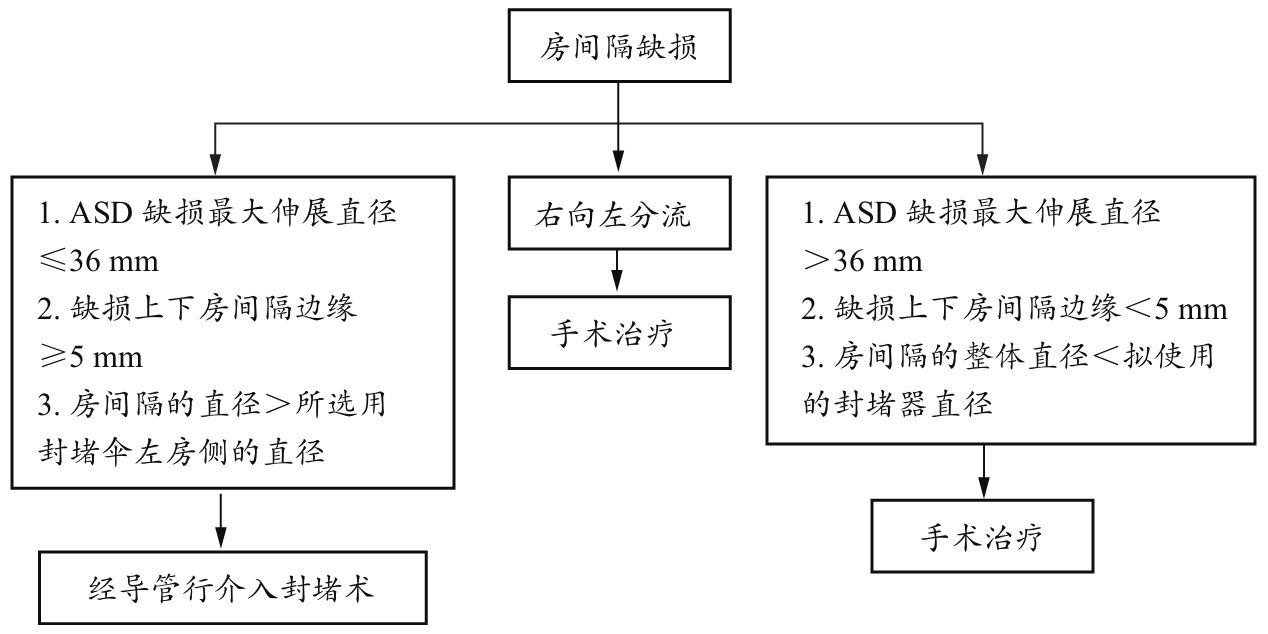
\includegraphics{./images/Image00077.jpg}
 \captionsetup{justification=centering}
 \caption{房间隔缺损的治疗程序}
 \label{fig2-9-1}
  \end{figure} 

【治疗方案】

1.
内科治疗 ①避免劳累及受凉感冒,预防和治疗并发症(如呼吸道感染、心力衰竭等)。②合并心房颤动时,应在正规抗凝治疗后进行心脏复律以恢复窦性心律,若患者通过药物或介入方法无法维持窦性心律,应进行心室率控制及抗凝治疗(Ⅰ/A)。

2. 介入封堵治疗

(1)适应证:①年龄:通常≥3岁。②直径≥5mm,伴右心容量负荷增加,≤36mm的继发孔型左向右分流ASD。③缺损边缘至冠状静脉窦,上、下腔静脉及肺静脉的距离≥5mm;至房室瓣≥7mm。④房间隔的直径\textgreater{}所选用封堵伞左房侧的直径。⑤不合并必须外科手术的其他心脏畸形。

(2)禁忌证:①原发孔型ASD及静脉窦型ASD。②心内膜炎及出血性疾患。③封堵器安置处有血栓存在,导管插入处有静脉血栓形成。④严重肺动脉高压导致右向左分流。⑤伴有与ASD无关的严重心肌疾患或瓣膜疾病。

3.
外科手术 ①3岁左右,合并肺动脉压增高、早期心力衰竭者应尽早手术。②静脉窦型、冠状静脉窦型或原发孔型ASD应行手术修补治疗。

【疗效观察与随访】

1. 观察指标 临床症状、体征、心电图、超声心动图、X线胸片等。

2.
疗效观察 根据多普勒左向右分流信号判定,无左向右分流信号为效果佳;直径\textless{}1mm左向右分流信号为微量残余分流;直径1\textasciitilde{}2mm为少量残余分流。

3.
随访 ①24小时内复查超声心动图。②术后24小时,1、3、6及12个月复查超声心动图、心电图及X线胸片。

【治疗经验与解析】

1. 不典型ASD或合并其他畸形,应行心导管检查。

2.
大多数患者可根据TTE测值推算出ASD直径,由于个体差异较大,术中球囊测量不应省略。

3. 对于ASD解剖较复杂,缺损太大、多孔型ASD应采用TEE监测完成介入封堵术。

4.
ASD合并重度肺动脉高压者较少,若合并重度肺动脉高压,应排除是否合并潜在的、未被发现的肺血管损害。

{(二)室间隔缺损}  室间隔缺损(ventricular septal
defect,VSD)是指在左、右心室之间存在一直接开口,是一种发病率最高的心脏畸形,大部分不能自行闭合而需临床治疗。室间隔解剖上由流入道、肌小梁、流出道三部分构成,分为三型:Ⅰ型肌型缺损,指缺损周边均为肌肉结构,可位于以上三部分中的任何一部分;Ⅱ型膜周部缺损,指缺损周边除肌肉结构外,一部分由房室瓣或动脉瓣间延伸的纤维组织构成,亦可见于以上三部分中的任何一部分;Ⅲ型为动脉瓣下缺损,缺损周边主要由主、肺动脉瓣延伸的结缔组织构成,仅见于流出道,室间隔缺损将导致心室水平的左向右分流,肺循环血量增加,肺动脉压力增高,早期肺血管阻力呈功能性增高,随着时间推移,肺血管发生组织学改变,形成肺血管梗阻性病变,可使右心压力逐步升高超过左心压力,转变为右向左分流,形成Eisenmenger综合征。

【治疗程序】 如图\ref{fig2-9-2}所示。

\begin{figure}[!htbp]
 \centering
 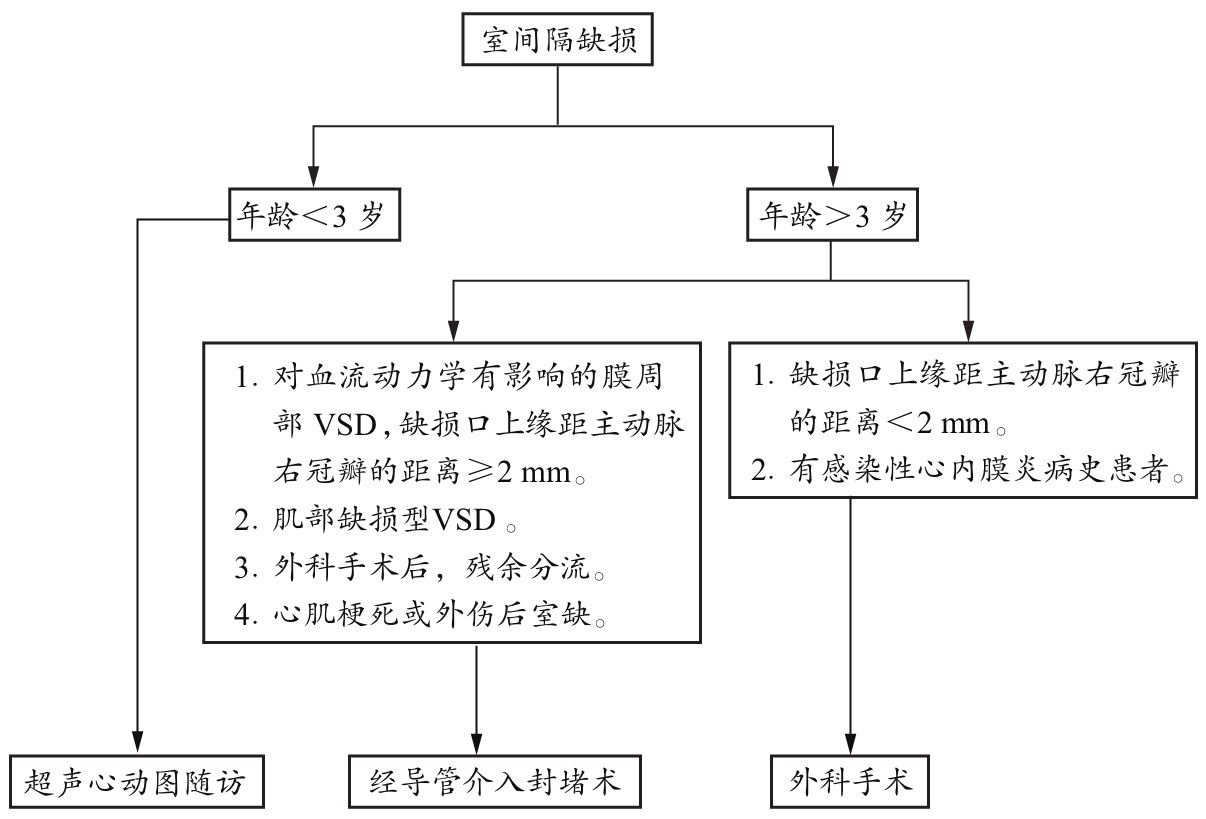
\includegraphics{./images/Image00078.jpg}
 \captionsetup{justification=centering}
 \caption{室间隔缺损的治疗程序}
 \label{fig2-9-2}
  \end{figure} 

【治疗方案】

1.
内科治疗 ①3岁以内VSD有40\%\textasciitilde{}60\%自然闭合率,故对于\textless{}3岁的患儿可临床随访,定期复查超声心动图。②合并进行性或严重肺血管疾病的VSD成年患者,可使用肺动脉扩张剂治疗。

2. 介入治疗

(1)适应证:①膜周部VSD:年龄通常≥3岁。对心脏有血流动力学影响的单纯性VSD。VSD上缘距主动脉右冠瓣≥2mm,无主动脉右冠瓣脱入VSD及主动脉瓣反流。②肌部室间隔缺损,通常≥5mm。③室间隔缺损外科手术后残余分流。④其他:心肌梗死或外伤后的室间隔缺损,也可采用先心病VSD的封堵技术进行封闭术,因局部心肌组织坏死,难以置放封堵器。必要时外科手术封堵。

(2)禁忌证:①相对禁忌证为不符合上述条件的单纯VSD。②绝对禁忌证为已有右向左分流。

3.
外科手术 ①对于肺循环与体循环血流比值(Qp/Qs)≥2.0,且临床检查证实存在左室容量超负荷患者,应予以外科手术。②有感染性心内膜炎病史。③肺动脉压低于全身血压的2/3、肺血管阻力小于全身血管阻力的2/3、Qp/Qs\textgreater{}1.5且存在单纯左向右分流的患者。④左室收缩或舒张功能衰竭、Qp/Qs\textgreater{}1.5且存在单纯左向右分流的患者。

【疗效观察与随访】

1. 观察指标 临床症状、体征、超声心动图、X线胸片等。

2.
疗效观察 封堵器安置后在TTE/TEE及左室造影下观察,封堵器安置位置恰当;无或仅有少量分流;无明显主动脉瓣及房室瓣反流,可判断为疗效良好。

3.
随访 ①24小时内复查超声心动图。②术后1、3、6和12个月随访,复查心电图、X线胸片及超声心动图。

【治疗经验与解析】

1.
典型的室间隔缺损一般不需要进行心导管检查及心血管造影。如疑有多孔缺损(室间隔上不止一个缺损口)或合并有其他先天畸形时应进行导管介入检查,对较大缺损已有继发性肺动脉病变,决定手术治疗时应行心导管检查,并进行肺动脉扩张药物试验。

2.
导管介入治疗后可发生各种心律失常,特别是束支传导阻滞及房室传导阻滞,其中房室传导阻滞可延迟发生,部分患者可于术后1周发生,故所有患者应于术后观察1周方可出院。

3.
合并严重PAH(艾森曼格综合征)的ASD女性患者由于母亲和胎儿死亡率较高,故不推荐妊娠,医生应强烈劝阻其妊娠。

{(三)动脉导管未闭}

动脉导管连接肺动脉总干与降主动脉,是胎儿期血液循环的主要渠道。出生后一般在数月内因废用而闭塞,如1岁后仍未闭塞,即为动脉导管未闭(Patent
ductus
arteriosus,PDA)。在先天性心脏病中占10\%左右。分流量小,临床上可无症状,突出体征为胸骨左缘第2肋间及左锁骨下方可闻及连续性机械样杂音,可伴有震颤。中等分流量患者常有乏力、劳累后心悸、气喘胸闷等症状;有时可在心尖部闻及由于左室扩大二尖瓣相对关闭不全及(或)狭窄所致的轻度收缩期及(或)舒张期杂音,周围血管征阳性。分流量大的未闭动脉导管,常伴有继发性严重肺动脉高压者可导致右向左分流。上述典型杂音的舒张期成分减轻或消失,继之收缩期杂音亦可消失,仅可闻及肺动脉瓣关闭不全所致的舒张期杂音,此时患者多有青紫,临床症状严重。

【治疗方案】

1. 内科治疗 预防并发症(感染、心衰等)。早产儿可采用消炎痛闭合PDA。

2.
介入治疗 主要包括最早的Porstmann栓塞法及后来的Rashkind双面伞法、Sideris纽扣法、Cook及PFM弹簧圈法。目前临床应用最广且操作简单的是Amplatzert蘑菇伞法。

(1)适应证:①左向右分流不合并需外科手术的心脏畸形的PDA。PDA最窄直径≥2mm,年龄通常≥6个月,体重≥4kg。②外科术后残余分流。

(2)禁忌证:①依赖PDA存在的心脏畸形。②严重肺动脉高压并已导致右向左分流。③败血症,封堵术前1个月内患有严重感染。

【疗效观察与随访】

1. 观察指标 临床症状、体征、超声心动图、X线胸片等。

2.
疗效观察 封堵器或弹簧栓子介入封堵术后,经主动脉弓降部造影观察如无或仅有少量残余分流为效果良好。

3.
随访 ①术后24小时,1、3、6及12个月复查超声心动图、心电图及X线胸片。②无左心容量超负荷的小型PDA患者,应接受常规随访;有左心容量超负荷的小型PDA患者,应每3\textasciitilde{}5年随访1次。

【治疗经验与解析】

1.
年龄越小PDA弹性越好者,选择略大的封堵伞,也要考虑到主动脉端大小,使主动脉端的伞尽量在PDA漏斗内,以免突出至主动脉内造成动脉狭窄。

2.
对合并重度肺动脉高压的患者,封堵器放置后肺动脉压力下降也可行封堵治疗,并能获得较好的远期疗效。

3. 已接受修补,无残余分流的PDA,无需预防感染性心内膜炎。

\subsection{有右至左分流的先天性心脏病}

{(一)法洛四联症}  先天性法洛四联症(congenital tetralogy of
Fallot)是联合的先天性心血管畸形,包括肺动脉口狭窄、心室间隔缺损、主动脉右位(主动脉骑跨于缺损的室间隔上)、右室肥大四种异常,是最常见的紫绀型先天性心脏病,在成人先天性心脏中所占比例接近10\%。本症主要畸形为室间隔缺损,均为大缺损,多为膜周部,左、右心室压力相等。本症常可伴发其他畸形,如同时有房间隔缺损则称之为法洛五联症。临床症状主要是自幼出现的进行性青紫和呼吸困难,易疲乏,劳累后常取蹲踞位休息。严重缺氧时可引起晕厥,长期右心压力增高及缺氧可发生心功能不全。患者除明显青紫外,常伴有杵状指(趾),心脏听诊肺动脉瓣第二心音减弱以致消失,胸骨左缘常可闻及收缩期喷射性杂音。脑血管意外(如脑梗死)、感染性心内膜炎、肺部感染为本病常见并发症。

【治疗方案】

1. 一般治疗 多喝水,预防感染、贫血等。

2.
缺氧发作的治疗 ①膝胸位,吸氧。②安定、鲁米那、吗啡等镇静。③β受体阻滞剂:心得安、甲氧乙心安。④纠正酸中毒。⑤纠正缺氧发作的诱因:感染、贫血、酸中毒等。

3.
外科治疗 ①根治术:1\textasciitilde{}2岁,严重者半岁前也可手术。②姑息手术,分流术等。

【疗效观察与随访】

1. 观察指标 临床症状、体征、心电图、超声心电图、X线胸片等。

2. 疗效观察 修补术后患者症状改善,手术成功,考虑疗效满意。

3.
随访 术后1、3、6及12个月随访,包括临床检查、心电图、X线胸片及超声心动图。

【治疗经验与解析】

1. 行主动脉瓣球囊成形术的患者,远期效果大多不好,多需行外科手术治疗。

2.
本病易患感染性心内膜炎,病情可因此急剧恶化。故术后6个月给予肠溶阿司匹林每日3\textasciitilde{}5mg/kg口服,术前1至术后3日静脉使用抗生素预防感染。术后6个月内常规预防感染性心内膜炎。

3.
主动脉二叶瓣畸形患者,如出现突发剧烈胸痛症状时,无论有无瓣膜功能不全,应考虑主动脉夹层的可能。

{(二)三尖瓣下移畸形}
 先天性三尖瓣下移畸形多称之为埃勃斯坦畸形(Ebstein
anomaly),是一种少见复杂先天性心脏畸形,占先天性心脏病的0.5\%\textasciitilde{}1.0\%,其主要病变为三尖瓣瓣叶及其附着部位的异常,前瓣叶大多附着于瓣环的正常部位,而膈瓣叶和后瓣叶发育不良且附着部位不在瓣环位置而下移至右心室心尖部,伴有三尖瓣关闭不全。这类畸形几乎均合并卵圆孔未闭或房间隔缺损。部分患者存在右侧房室旁路。患者自觉症状轻重不一,可有心悸、气喘、乏力、头晕和右心衰竭等。约80\%患者有青紫,有20\%患者有阵发性房室折返性心动过速病史。最突出的体征是心界明显增大,心前区搏动微弱。心脏听诊可闻及四音律,胸骨左缘下端可闻及三尖瓣关闭不全的全收缩期杂音,颈动脉扩张性搏动及肝脏肿大伴扩张性搏动均可出现。

【治疗方案】 Ebstein心脏畸形患者如属轻型、无临床症状者,可随访观察。有症状者首选房化心室折叠。如胸部X线片提示心脏明显增大、症状重者,需手术治疗。

【疗效观察与随访】

1. 观察指标 临床症状、体征、心电图、超声心动图、X线胸片等。

2. 疗效观察 外科手术后临床症状改善,无或轻度瓣膜反流,则为显效。

3.
随访 术后1、3、6及12个月随访,包括临床检查、心电图、X线胸片及超声心动图。

【治疗经验与解析】

1. 对轻型及中间型首选房化心室折叠及三尖瓣成形术。

2.
部分重症病例,右心室发育差,功能严重受损,术中可见整个右心室壁包括三尖瓣异常附着处的近心端及漏斗部均变薄扩张,显著凸起,对这类病例,多采取同时做双向腔肺动脉分流,以减轻右心负担,即1/2心室修补术(一室半术)。

3.
对于心脏显著扩大,三尖瓣发育极差,尤其前瓣或瓣下结构与右心室融合,影响前瓣活动;或前瓣虽然宽大,但过大的前瓣脱至右室流出道影响血流动力学者,应考虑行三尖瓣置换。

4.
对于功能不良右心室、右心室流出道相对狭窄、三尖瓣前瓣发育差的重症患者,可应用房间隔造口技术,安置可调试房间隔造口术。

5.
超声检查是目前准确有效的诊断方法,应当避免心导管检查,因为在操作过程中可导致严重的快速性心律失常。

{(三)艾森曼格综合征}  艾森曼格综合征(Eisenmenger
syndrome)为一组先天性心脏病发展的后果,如先天性室间隔缺损持续存在,可由原来的左向右分流,由于进行性肺动脉高压发展至器质性肺动脉阻塞性病变,出现右向左分流,从无青紫发展至有青紫时,即称之为Eiesenmenger综合征。其他如房间隔缺损、动脉导管未闭等也可有类似情况。临床表现为轻至中度青紫,于劳累后加重,逐渐出现杵状指(趾),常伴有气急、乏力、头晕等症状,以后可出现右心衰竭的相关症状。体征示心浊音界明显增大,心前区胸骨左缘3\textasciitilde{}4肋间有明显搏动,原有左向右分流的杂音减弱或消失(动脉导管未闭的连续性杂音中,舒张期部分可消失),肺动脉瓣第二心音亢进、分裂,以后可出现舒张期杂音,胸骨下段偏左部位可闻及收缩期反流性杂音。

【治疗方案】

1. 一般治疗

(1)吸氧:有利于减轻PAH患者肺血管痉挛。降低肺血管阻力,一般用于治疗低氧血症[血氧饱和度(SaO{2}
)动脉血\textless{}91\%]和急性PAH。

(2)一般治疗药物:

洋地黄类:心排出量低于4L/min或心排血指数\textless{}2.5L/(min·m{2}
)者可应用地高辛;右心室明显扩张。基础心率\textgreater{}100次/分钟,尤其合并心室率偏快的心房颤动(房颤)患者是应用地高辛的绝对指征。

利尿剂:对于合并右心功能不全的PAH患者。初始治疗应给予利尿剂。

抗凝剂:对预防血栓形成可能有一定作用。在女性和SaO{2}
偏低患者意义更大,但应注意防止出血、咯血等并发症;应用华法林时宜将国际标准化比值(INR)控制在1.5\textasciitilde{}2.0。

Ca{2+}
通道拮抗剂:强调用药前进行急性血管扩张试验,试验阳性患者从小剂量开始。逐渐达到最大耐受剂量;除硝苯地平外,氨氯地平、非洛地平等长效制剂也可应用;长期大剂量用药易出现低血压、负性肌力作用等不良反应。不少患者可能难以耐受。

2. 靶向治疗药物

(1)ET受体拮抗剂:波生坦(Bosentanl)作为一种口服的竞争性ET受体拮抗剂。对ETA和ETB受体均有阻滞效应。

(2)PDE-5抑制剂:环磷酸鸟苷(cGMP)是细胞内介导血管扩张和平滑肌增殖的第二信使,促进肺血管扩张和抗增殖效应。

(3)PGl2类:对VSMCs具有舒张作用,可抑制血管平滑肌的增生,逆转血管重构,恢复损伤的血管内皮细胞功能,抑制血小板聚集PGl2类药物依前列醇在PAH治疗中已显示出较好的临床应用前景。

(4)一氧化氮(NO):使总肺血管阻力下降,改善生存率。

3.
心肺联合移植 艾森曼格综合征为先天性心脏病后期,已失去手术治疗机会,预后不良。有条件者可行心肺联合移植。

【疗效观察与随访】

1. 观察指标 临床症状、体征、心电图、超声心动图、X线胸片等。

2. 疗效观察 药物治疗后观察肺动脉压力,肺动脉压力降低20\%,提示有效。

3. 随访 定期检查心电图、X线胸片及超声心动图。

【治疗经验与解析】 药物治疗效果差,手术治疗成功率低,预后差。


\section{感染性心内膜炎}

感染性心内膜炎(infective
endocarditis,IE)为心内膜、心瓣膜或邻近大动脉内膜表面的微生物感染并伴赘生物形成。多发生于已有基础心脏病者。瓣膜为最常受累部位,但感染也可发生在间隔缺损部位、腱索或心壁内膜。根据感染部位及是否存在心内异物,IE分为左心自体瓣膜IE、左心人工瓣膜IE、右心IE和装置相关性IE。链球菌和葡萄球菌是最常见的致病菌。IE的诊断依赖于血培养阳性、超声心动图(赘生物、脓肿、人工瓣膜裂开)和临床表现。IE常导致心力衰竭、心律失常、栓塞等并发症。

【治疗方案】

{(一)药物治疗}

1. 用药原则

(1)早期应用:在连续送3\textasciitilde{}5次血培养后即可开始治疗。

(2)充分用药:选用杀菌性抗微生物药物,大剂量和长疗程,旨在完全消灭藏于赘生物内的致病菌。

(3)静脉用药为主:有利于保持高而稳定的血药浓度。

(4)病原微生物不明时:选用针对金黄色葡萄球菌、链球菌和革兰阴性杆菌均有效的广谱抗生素。

(5)已分离出病原微生物时:应根据致病微生物对药物的敏感程度选择抗微生物药物。

2.
初始经验性抗菌治疗 需考虑患者此前是否接受过抗菌治疗,感染累及自体瓣膜或人工瓣膜,如为后者,何时进行手术,当地病原微生物流行情况,特别是耐药菌、血培养阴性菌。①在病原菌尚未培养出时,可予萘夫西林2g,每4小时1次,静脉注射或滴注,加氨苄西林2g,每4小时1次,静脉注射,或加庆大霉素每日160\textasciitilde{}240mg静脉注射。②考虑为链球菌感染者,可予青霉素320万\textasciitilde{}400万U静脉滴注,每4\textasciitilde{}6小时1次,或加庆大霉素(剂量同上)。

3. 已知致病微生物时的治疗

(1)对青霉素敏感的链球菌(MIC≤0.1mg/L):首选青霉素1200万\textasciitilde{}1800万U/d,分次静脉滴注,每4小时1次;或青霉素联合庆大霉素1mg/kg静脉注射或肌内注射,每8小时1次;青霉素过敏时可选择头孢曲松2mg/d,静脉注射或万古霉素30mg/(kg·d),分2次静脉滴注(24小时最大量不超过2g)。所有病例均至少用药4周。

(2)对青霉素耐药的链球菌(MIC\textgreater{}1mg/L):青霉素加庆大霉素,青霉素1800万U/d,分次静脉滴注,每4小时1次,用药4周,庆大霉素剂量同前,用药2周;青霉素过敏时万古霉素加庆大霉素,剂量疗程同前。

(3)葡萄球菌(甲氧西林敏感):①萘夫西林或苯唑西林均为2g,每4小时1次,静脉滴注,用药4\textasciitilde{}6周;治疗初始3\textasciitilde{}5日加用庆大霉素,剂量同前。②青霉素过敏或无效者用头孢唑林2g静脉注射,每8小时1次,用药4\textasciitilde{}6周;治疗初始3\textasciitilde{}5日加用庆大霉素。③如青霉素和头孢菌素无效,可用万古霉素4\textasciitilde{}6周。

(4)葡萄球菌(甲氧西林耐药):万古霉素加利福平及庆大霉素,万古霉素剂量同前,利福平1200mg/d,静脉滴注或口服,分2次给药,均至少治疗6周。庆大霉素剂量同前,治疗2周。

(5)肠球菌:①青霉素加庆大霉素,青霉素1800万\textasciitilde{}3000万U/日,分次静脉滴注,每4小时1次。庆大霉素用量同前,疗程4\textasciitilde{}6周。②氨苄西林加庆大霉素,氨苄西林12g/d,分次静脉注射,每4小时1次,庆大霉素剂量同前,疗程4\textasciitilde{}6周,治疗过程中酌减或撤除庆大霉素,预防其不良反应。③对青霉素过敏者,万古霉素加庆大霉素,万古霉素30mg/(kg·d),分2次静脉滴注,疗程6周。

(6)真菌感染:静脉滴注两性霉素B,首日0.02\textasciitilde{}0.1mg/kg,之后每日递增3\textasciitilde{}5mg,直至25\textasciitilde{}30mg/d,总量3\textasciitilde{}5g,注意药物不良反应。疗程满后口服氟胞嘧啶100\textasciitilde{}150mg/(kg·d),每6小时1次,用药数月。

{(二)手术治疗}

1.
活动性自体瓣膜心内膜炎的手术指征 ①急性主动脉瓣反流所致心衰者。②急性二尖瓣反流所致心衰者。③尽管积极抗生素治疗情况下,菌血症和发热持续8日以上。④脓肿、假性动脉瘤以及1个(多个)瓣叶破裂或瘘引起异常交通的征象表明局部感染扩散(局部感染未控制)时。⑤不容易治愈(如真菌、布鲁菌和Q热病原体)或对心脏结构破坏力大的病原微生物感染时。

2.
手术治疗 ①二尖瓣赘生物\textgreater{}10mm或抗生素治疗下赘生物体积增大或赘生物位于二尖瓣闭合的边缘时应考虑尽早手术治疗。②复发的肺动脉栓塞后三尖瓣赘生物\textgreater{}20mm时必须手术治疗。

【疗效观察与随访】

1.
观察指标 症状、体征(监测体温、脉搏、心率、呼吸、血压、尿量,心脏杂音、两肺呼吸音、皮肤粘膜等的变化)及血象、C反应蛋白、肾功能、血培养、心电图、超声心动图等。

2. 疗效观察 治愈标准:症状、体征消失,血培养连续3次阴性,无并发症。

3. 随访

(1)对患者进行健康教育,使其了解感染性心内膜炎的症状和体征,以便患者能意识到感染再发。

(2)随访晚期并发症,包括感染再发、心力衰竭、是否需要进行瓣膜手术及生存率。

(3)出院后第1、3、6、12个月复诊,进行实验室检查(白细胞、C反应蛋白)和超声心动图检查,评估患者的临床状况。

【治疗经验与解析】

1.
对于可能出现IE不良预后的高危患者,在进行所有涉及牙龈组织、牙根尖周或穿破口腔粘膜的牙科操作时,推荐IE预防。

2.
IE高危患者包括:①有人工心脏瓣膜或应用人工材料进行瓣膜修复的患者。②既往有IE病史者。③特定的先天性心脏病患者,包括未修补的紫绀型先天性心脏缺损患者,用人工材料或装置经手术或介入方式进行完全修补术后6个月内、经修补后在原部位或邻近人工补片或装置附近有残余缺损者。④心脏移植后发生瓣膜病变者(因瓣膜结构异常引起反流)。

3.
对不伴活动性感染的患者,如进行不穿透粘膜的非牙科操作(例如TEE、诊断性支气管镜、食管胃镜或结肠镜),不推荐IE预防。

4.
当β内酰胺类抗生素需要合并氨基糖苷类时都选择庆大霉素,但在我国庆大霉素发生耐药率高,而且庆大霉素肾毒性大,故多选用肾毒性较小的阿米卡星替代庆大霉素,剂量为0.4\textasciitilde{}0.6g/d,分次静脉注射或肌内注射。


\section{心包炎}

心包炎按病情进展,可分为急性心包炎(伴或不伴心包积液)、慢性心包积液、粘连性心包炎、亚急性渗出性缩窄性心包炎、慢性缩窄性心包炎等。临床上以急性心包炎和慢性缩窄性心包炎为最常见。

\subsection{急性心包炎}

急性心包炎为心包脏层和壁层的急性炎症,病因有感染性、自身免疫性、代谢性疾病、肿瘤性疾病、药物反应性疾病、创伤、邻近器官病变、放射性以及结节病、淀粉样变性、肠道感染性疾病、贝切赫病等。根据病理变化,急性心包炎可分为纤维蛋白性(也是最常见的临床病理表现)和渗出性。心包积液可在数周至数月内吸收,但也可伴随发生壁层与脏层的粘连、增厚及缩窄,也可在较短时间心包内大量液体积聚引起心脏压塞。

【治疗程序】 如图\ref{fig2-11-1}所示。

\begin{figure}[!htbp]
 \centering
 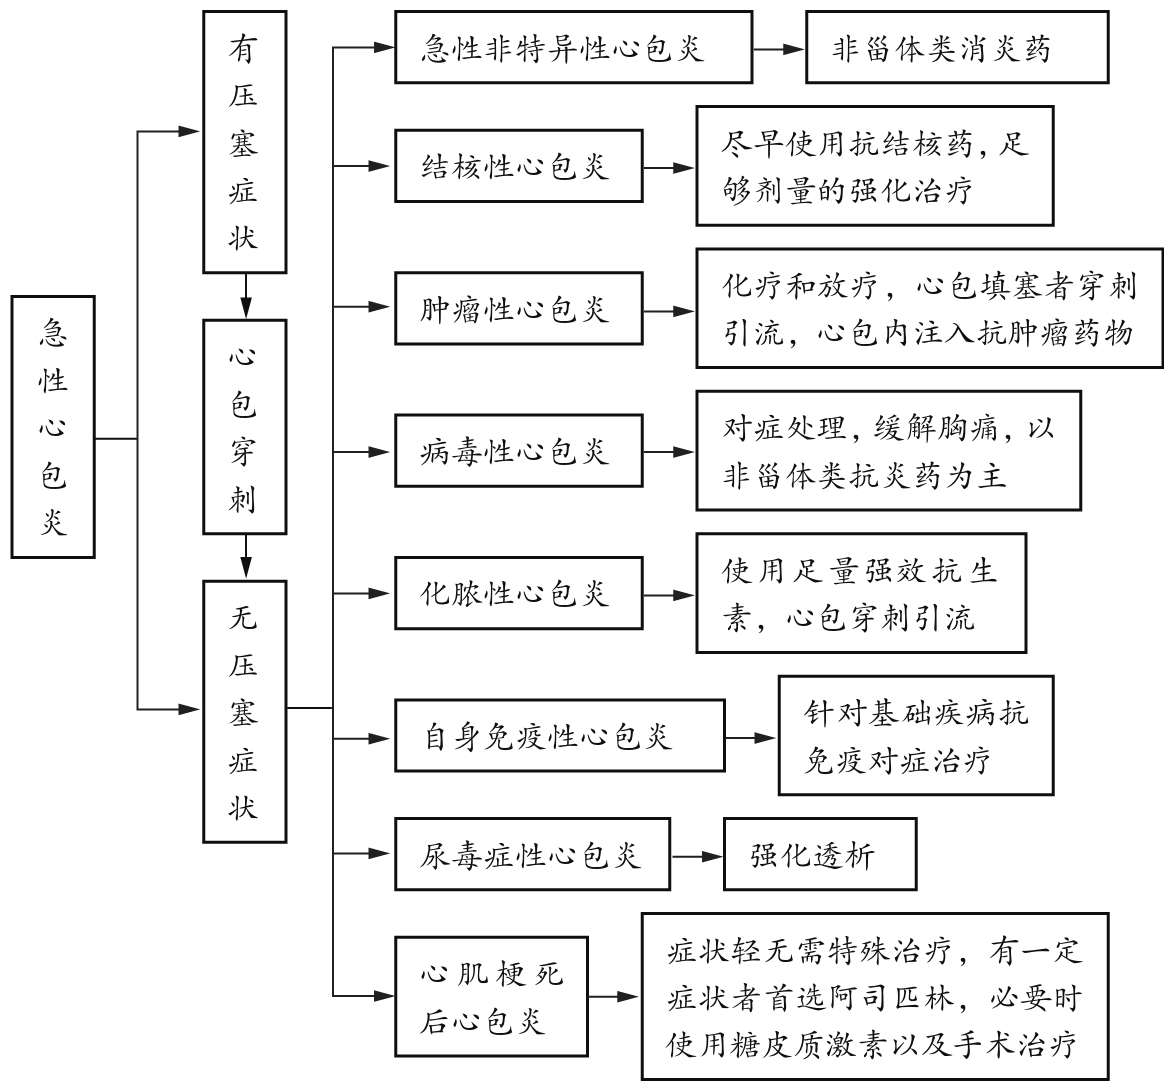
\includegraphics{./images/Image00079.jpg}
 \captionsetup{justification=centering}
 \caption{急性心包炎的治疗程序}
 \label{fig2-11-1}
  \end{figure} 

【治疗方案】

1. 大量心包积液 如导致心脏压塞,影响血流动力学,予以紧急心包穿刺术。

2.
急性非特异性心包炎 卧床休息,镇痛,对症处理,使用非甾体类消炎药,首选布洛芬300\textasciitilde{}800mg,每日3次,或阿司匹林300\textasciitilde{}600mg,4\textasciitilde{}6小时1次,或吲哚美辛25\textasciitilde{}50mg,每日3次,注意预防胃粘膜损害。

3.
结核性心包炎 应尽早使用抗结核药,足够剂量的强化治疗,异烟肼、利福平、吡嗪酰胺、乙胺丁醇联合用药,早期应用足量糖皮质激素,复发性积液或缩窄性心包炎可开窗引流活检,缩窄性心包炎可在结核控制后手术治疗。

4.
肿瘤性心包炎 治疗方案依据肿瘤的组织学以及基础情况决定,确定抗肿瘤治疗,包括化疗和放疗,心包填塞者穿刺引流,大量积液高复发者持续引流或心包内注入细胞生长抑制药物以及硬化剂,以缓解症状和改善生活质量为目标。

5.
病毒性心包炎 主要对症处理,缓解胸痛,以非甾体类抗炎药为主,心包积液多数无需特殊处理,重症者肾上腺皮质激素治疗,AIDS患者心包炎预后差,除特异治疗外,需抗结核治疗。

6.
尿毒症性 应强化透析,如无效则非肝素化腹膜透析,并使用NSAIDS以及皮质激素全身治疗,心包填塞予以心包穿刺,顽固大量心包积液心内滴注皮质激素治疗。

7.
自身免疫性心包炎 针对基础疾病抗免疫对症治疗,早期使用泼尼松、布洛芬、秋水仙碱,逐渐减量。必要时心包内注入不易吸收的激素,如氟羟强的松龙。

8.
化脓性心包炎 根据药敏静脉使用足量有效抗生素,心包穿刺引流,必要时尿激酶、链激酶冲洗。

9.
心肌梗死后心包炎 症状轻无需特殊治疗,有一定症状者首选阿司匹林600mg,每6\textasciitilde{}8小时1次,皮质激素用于心梗缓解但心包炎顽固复发仍有胸痛者。心包破裂者紧急手术。

【疗效观察与随访】

1.
观察指标 观察治疗前后患者的症状、体征变化,如胸痛的部位、持续时间,疼痛特点,呼吸困难的程度,心包摩擦音、心包积液的变化等。

2. 治愈标准 症状、体征消失、3个月内未复发。

3.
随访 半年内可予心电图、超声心动图、X线胸片、MRI等动态监测。亦可予心包穿刺、纤维心包镜、血常规、血沉、C反应蛋白、心肌损伤标记物、PPD试验等检查。

【治疗经验与解析】

1.
应针对原发疾病行病因治疗,解除心脏压塞和对症治疗。患者必须住院观察,卧床休息,胸痛时给予镇静剂、阿司匹林、布洛芬,必要时可使用吗啡类药物。

2.
急性心包炎的自然病程及预后取决于病因,病毒性心包炎、心肌梗死后心包炎等通常是自限性的,临床表现可在2\textasciitilde{}6周消退。若心包炎并发于恶性肿瘤、系统性红斑狼疮、尿毒症等,则预后差。化脓性或结核性心包炎随着抗生素或抗结核药物应用以及外科手术的进展,预后已大为改善,部分患者遗留心肌损害或发展为缩窄性心包炎。

\subsection{缩窄性心包炎}

缩窄性心包炎是指心脏被致密厚实的纤维化或钙化心包所包围,使心室舒张期充盈受限而产生一系列循环障碍的病征。继发于急性心包炎,病因在我国仍以结核性为最常见,其次为急性非特异性心包炎、化脓性或创伤性心包炎后演变而来。放射性心包炎和心脏直视手术后引起者逐渐增多。少数与心包肿瘤等有关。可导致心脏及大血管根部受限,心包缩窄使心室舒张期扩张受阻,心室舒张期充盈减少,使心搏量下降。上、下腔静脉回流受阻,静脉压升高、颈静脉怒张、肝大、腹水、下肢水肿等。常见症状为呼吸困难、疲乏、食欲不振、上腹胀满或疼痛。

【治疗方案】 早期施行心包剥离术或心包切除术以避免发展到心源性恶病质、严重肝功能不全、心肌萎缩等。通常在心包感染被控制、结核活动已静止即应手术,并在术后继续用药1年。

【疗效观察与随访】

1.
观察指标 临床症状与体征、心脏压塞征、X线胸片、超声心动图、心包液培养及常规检查。

2. 疗效观察

治愈标准 症状、体征消失,心脏压塞征解除,各项相关检查指标正常。

好转标准 症状、体征基本消失,相关检查指标未能完全恢复正常。

3.
随访 重点随访好转病例是否完全恢复,定期行X线胸片和超声心动图检查,其他如血象、血沉的检查等。

【治疗经验与解析】

1. 必须迅速查明病因,针对病因进行治疗。

2.
本病一旦确诊,应及时行心包剥离或切除术,手术宜在病程早期施行,病程过久,患者营养及一般情况不佳,心肌常有萎缩和纤维变性,即使心包剥离成功,也会因心肌不健全而影响手术效果。心包穿刺也是一项关键性的治疗。

3.
目前不主张心包腔内注入抗生素的治疗,因为静脉滴注抗生素可以达到治疗浓度。

4.
吲哚美辛、布洛芬和糖皮质激素有增加心脏破裂的危险,近来提倡需要使用时,可用阿司匹林代替。


\section{病毒性心肌炎}

病毒性心肌炎(viral
myocarditis)是指嗜心肌病毒感染引起的以心肌非特异性间质性炎症为主要病变的心肌炎。主要病原是柯萨奇B组2\textasciitilde{}5型和A组9型病毒,其次是埃可病毒和腺病毒。病毒性心肌炎可为流行发病,在病毒流行感染期约有5\%的患者发生心肌炎,也可为散在发病。临床表现从心肌局灶炎症无症状到心肌弥漫性炎症所致的重症心肌炎。41\%\textasciitilde{}88\%患者有前驱病毒感染史。临床观察1个月,异常体征消失属轻症;重症心肌炎病程约需3个月,大多数患者可完全恢复。

【治疗方案】

1.
一般治疗 ①急性病毒性心肌炎患者尽早卧床休息,可以减轻心脏负荷。②有严重心律失常、心衰的患者,卧床休息1个月,半年内不参加体力活动。③无心脏形态功能改变者,休息半个月,3个月内不参加重体力活动。

2. 抗病毒治疗

(1)α-干扰素:能够阻断病毒复制和调节细胞免疫功能。用法:100\textasciitilde{}300万U,每日1次肌内注射,2周为一个疗程。

(2)黄芪:有抗病毒、调节免疫功能及对干扰素系统有激活作用。用法:黄芪注射液20g+5\%葡萄糖注射液250ml,静脉滴注,每日1次,2周为一个疗程,然后改为口服黄芪治疗。

3. 保护心肌疗法

(1)维生素C:保护心肌不受自由基和脂质过氧化损伤作用。重症心肌炎患者,维生素C
5g+5\%葡萄糖注射液250ml,静脉滴注,每日1次,1\textasciitilde{}2周为一个疗程。

(2)辅酶Q10:参与氧化磷酸化及能量的生成过程,并有抗氧化自由基及膜稳定作用。辅酶Q10片10mg口服,每日3次,1个月为一个疗程。

(3)曲美他嗪:抑制游离脂肪酸β氧化,促进葡萄糖氧化,利用有限的氧,产生更多ATP,增加心脏收缩功能。曲美他嗪20mg口服,每日3次,1个月为一个疗程。

4.
免疫抑制剂治疗 在心肌炎早期患者出现完全性房室传导阻滞、严重室性心律失常、心源性休克、心脏扩大伴有心力衰竭等严重并发症,可以短期应用糖皮质激素治疗。

5. 对症治疗

(1)出现心力衰竭者:按常规心力衰竭治疗,但洋地黄用量宜偏小,贝那普利5\textasciitilde{}10mg或培哚普利2\textasciitilde{}8mg口服,每日1次。

(2)完全性房室传导阻滞者:使用临时体外起搏器,可短程应用地塞米松10mg静脉滴注,每日1次,3\textasciitilde{}7日,不能恢复者安装永久心脏起搏器。

(3)心律失常:根据心律失常情况选择抗心律失常药物治疗。

【疗效观察与随访】

1.
观察指标 ①轻症病例主要观察临床症状改善,复查血沉、血常规、血清心肌损伤标志物及心电图。②重症病例需密切观察心率、节律、呼吸、血压,心功能,肝肾功能,电解质及血气分析变化。③某些隐匿进展型心肌炎数年后可能出现心脏逐渐扩大,表现为扩张型心肌病,随访时注意定期复查胸片、超声心动图。

2.
治愈标准 症状、体征消失,心电图恢复正常,各项相关检查指标正常,3个月内无复发。

3. 随访 定期复查心肌酶谱、心电图、超声心动图、X线胸片等。

【治疗经验与解析】

1.
本病预后与其发病类型有关,大多数患者经过药物治疗后可完全康复,但由于治疗不及时可能遗留心律失常、心功能减退等后遗症。甚至极少数患者由于心肌弥漫性炎症与坏死及免疫介导的心肌损害,发生急性心力衰竭、心源性休克或严重心律失常而死亡。对于上述重症病例应早期明确诊断。

2.
对于心力衰竭者,虽可按照心力衰竭常规治疗,但洋地黄用量宜偏小。对于心源性休克,药物治疗无效时可早期尝试主动脉内球囊反搏。

3.
高度或完全性房室传导阻滞者,可采用临时体外起搏器或静脉滴注异丙肾上腺素治疗,在静脉滴注异丙肾上腺素治疗过程中,滴速过快或剂量过大可使心房率增加而不能增快心室率,反而由于隐匿性传导使房室传导阻滞加重;或因心室率增快而增加心肌应激性,引发致命的室性心动过速。

4.
室性心动过速时,应尽量减少抗心律失常药物的联合应用,纠正电解质紊乱及注意药物对心功能的影响;应用胺碘酮时预防血压下降;药物仍然不能纠正的室性心动过速或伴有血流动力学障碍需电复律时,一定要在临时起搏保护下进行,否则有心脏停搏的危险。

5.
肾上腺糖皮质激素应在下述情况时早期应用:①严重的毒血症;②心源性休克;③严重心力衰竭;④高度或完全性房室传导阻滞;⑤持续性室性心动过速或其他恶性室性心律失常。此时,应用糖皮质激素有利于局部炎症和水肿的消除,抑制过强的免疫反应。


\section{心肌病}

心肌病是指伴有心肌功能障碍的心肌疾病,不包括冠心病、高血压病、心脏瓣膜病、先天性心血管病所致的心肌病变,主要表现为心力衰竭、体循环栓塞、心律失常、猝死。原发性心肌病指病因未明的心肌病,分为扩张型心肌病、肥厚型心肌病、限制型心肌病、致心律失常型右室心肌病及未定型心肌病。特异性(继发性)心肌病病因明确,心肌病变作为全身多器官病变之一,如全身性疾病、中毒性疾病、内分泌疾病、自身免疫性疾病等累及心肌者。克山病(地方性心肌病)曾经在我国暴发流行,且有其特点,故列入特异性心肌病。

\subsection{扩张型心肌病}

扩张型心肌病(dilated
cardiomyopathy,DCM)主要特征是单侧或双侧心腔扩大,心肌收缩期功能减退,伴或不伴有充血性心力衰竭。病因迄今不明,除特发性、家族遗传性外,近年来认为持续病毒感染是其重要原因。本病起病缓慢,患者多在临床症状明显时方就诊,如有气急、端坐呼吸、水肿和肝大等充血性心力衰竭的症状和体征时,始被诊断。部分患者可发生栓塞或猝死。主要体征为心脏扩大,常可听到第三或第四心音,心率快时呈奔马律。常合并各种类型的心律失常,以室性心律失常或房性心律失常多见。

【治疗程序】 如图\ref{fig2-13-1}所示。

\begin{figure}[!htbp]
 \centering
 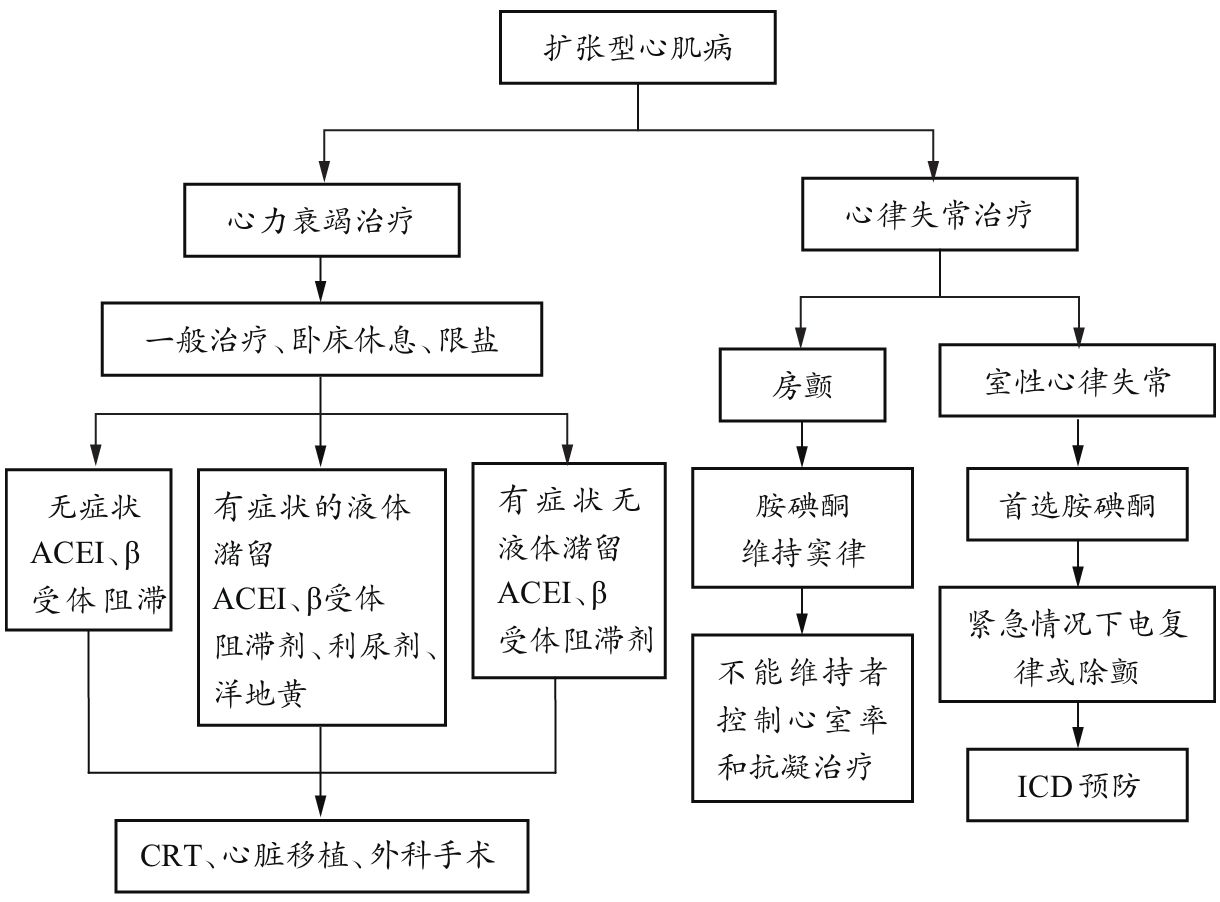
\includegraphics{./images/Image00080.jpg}
 \captionsetup{justification=centering}
 \caption{扩张型心肌病的治疗程序}
 \label{fig2-13-1}
  \end{figure} 

【治疗方案】

1. 一般治疗 休息及避免劳累,限制体力活动,低盐饮食,控制感染。

2. 控制心力衰竭治疗 原则和治疗一般心力衰竭相同。

(1)洋地黄和非洋地黄类制剂:由于心肌损害较广泛,较易发生洋地黄中毒,故应慎用。非洋地黄正性肌力药如肾上腺素受体兴奋剂和磷酸二酯酶抑制剂可短期应用。

(2)利尿剂:通常从小剂量襻利尿剂开始,如呋塞米每日20mg,并逐渐增加剂量至尿量增加,体重每日减轻0.5\textasciitilde{}1.0kg,一旦肺部啰音消失,水肿消退,体重稳定,即可以最小有效剂量长期维持,一般需无限期使用。但出现低肾小球滤过时,氢氯噻嗪可能失效,应选用襻利尿剂呋塞米等。

(3)醛固酮受体拮抗剂:螺内酯可阻断醛固酮效应,抑制心肌重构,对改善预后有益。

(4)扩血管药、ACEI:需要从小剂量开始,避免造成低血压。

(5)β受体阻滞剂:可使肾上腺素能神经过度兴奋的有害作用被去除,β受体密度上调,从而延缓病情进展。已知β{1}
选择性(如美托洛尔)和血管扩张作用者(如卡维地洛)效果较好,起始用极小剂量,然后缓慢加大剂量以靶剂量或最大耐受剂量长期维持。

(6)脑钠肽(BNP):有均衡扩张动静脉、利尿、增加心输出量作用,可用于治疗急性心力衰竭。

(7)钙拮抗剂:近年来报道如地尔硫䓬
也能改善心功能,应从小剂量开始。

3.
抗心律失常治疗 尤其有症状者需用抗心律失常药或电学方法治疗,对快速性心律失常或高度房室传导阻滞而有猝死危险者应积极治疗。

4.
抗凝治疗 有心腔明显扩大伴低射血分数、NYHAⅣ级、长期卧床,尤其有血管栓塞史或深静脉有血栓形成的患者可使用华法林抗凝,调节剂量使凝血酶原时间国际标准化比值(INR)保持在2\textasciitilde{}3。

5.
其他药物治疗 改善心肌代谢药物如维生素C、三磷腺苷、辅酶A、环磷腺苷、辅酶Q10可作为辅助治疗。抗病毒和免疫治疗药物如黄芪、生脉、牛磺酸、干扰素具有一定改善心功能及预后作用。

6.
心脏再同步化治疗(CRT)和心脏电复律除颤器(ICD) 主要用于用药效果不佳、左室射血分数(LVET)\textless{}30\%、QRS\textgreater{}120ms、呈完全性左束支传导阻滞或心室内传导阻滞患者。可通过双心室起搏器同步刺激左、右心室,调整左右心室收缩程序,改善心功能,缓解症状。对伴顽固持续快速室性心律失常患者可置入ICD以预防心性猝死。

7.
左室减容成形术 通过切除部分扩大的左心室,同时置换二尖瓣,以减轻反流、改善心功能,但术后心衰加重和心律失常的死亡率较高。

8.
移植 有报道干细胞移植可以改善心功能,但疗效不确切。心脏移植在纠正排斥1年后生存率可达85\%以上,但供体严重短缺。

9.
左心机械辅助循环 通过机械装置将左心室血液引入主动脉以减轻左心负荷,为晚期DCM患者维持全身循环、不能进行心脏移植患者的一种有效方法,但价格昂贵,应用有限。

【疗效观察与随访】

1.
观察指标 心率、心律、心电图、超声心动图、心功能、心肌酶谱、临床症状及体征等。

2.
疗效判定 本病疗效不够满意,目前尚缺乏治愈方法。本病的病程长短不等,充血性心力衰竭的出现频度较高,预后不良。死亡原因多为心力衰竭和严重心律失常,不少患者猝死。以往认为症状出现后5年的存活率在40\%左右。近年来,由于治疗进展其存活率已明显提高。

3.
随访 治疗后定期复查心肌酶谱、心功能、超声心动图、心电图等,密切观察病情变化。

【治疗经验与解析】

1.
所有症状性心力衰竭者,如无禁忌证,均应使用ACE抑制剂和β受体阻滞剂。伴有体液潴留者加用利尿剂。不能耐受ACE抑制剂和β受体阻滞剂者可考虑使用血管紧张素Ⅱ{1}
受体拮抗剂。

2.
当心力衰竭进展恶化时,大剂量利尿剂口服反应欠佳,采用呋塞米每小时1\textasciitilde{}5mg持续静脉滴注,或两种以上利尿剂联合使用,或短期应用小剂量多巴胺或多巴酚丁胺2\textasciitilde{}5μg(kg·min)以增加肾血流改善利尿剂疗效。

3.
近年研究证实,心脏再同步治疗(CRT),不但可以改善心力衰竭患者运动耐量和生活质量,且能延长生存时间,作为一种补充治疗,药物治疗仍是基础。

\subsection{肥厚型心肌病}

肥厚型心肌病(hypertrophic
cardiornyopathy,HCM)是以左心室(或)右心室肥厚为特征,常为不对称肥厚并累及室间隔,左心室血液充盈受阻、舒张期顺应性下降为基本病态的心肌病,分为梗阻性、非梗阻性肥厚型心肌病。通常认为是常染色体显性遗传疾病,为青年猝死的主要原因之一。患者多有心悸、胸痛、劳力性呼吸困难,流出道梗阻的患者可出现头晕、晕厥。常见体征有心界向左下扩大;流出道有梗阻者可在胸骨左缘第3\textasciitilde{}4肋间闻及较粗糙的喷射性收缩期杂音;心尖部也常闻及收缩期杂音。使用β受体阻滞剂、取下蹲位可使杂音减轻;给予洋地黄类、异丙肾上腺素、硝酸甘油片、站立位可因相反作用使杂音增强。

【治疗方案】

1. 治疗目标 解除症状和控制心律失常。

2. 药物治疗

(1)β受体阻滞剂:可使心肌收缩力减弱从而减轻流出道梗阻,减少心肌耗氧量,增加舒张期心室扩张,且能减慢心率增加心搏量。普萘洛尔10mg,每日3\textasciitilde{}4次,最多可达200mg/d,另外还可使用阿替洛尔、美托洛尔。

(2)钙离子拮抗剂:可通过负性肌力作用减轻心肌收缩。维拉帕米120\textasciitilde{}480mg/d,分3\textasciitilde{}4次口服,血压过低、房室传导阻滞、窦房结功能减退者慎用。也可使用地尔硫䓬
30\textasciitilde{}60mg,每日3次。钙离子拮抗剂常用于β受体阻滞剂疗效不佳或有支气管哮喘患者。

(3)抗心律失常药:可用于控制快速室性心律失常和心房颤动患者,常用胺碘酮,无效时可电复律。

(4)对于晚期充血性心力衰竭患者:治疗与其他病因所致心衰相同。

(5)对重症梗阻性肥厚型心肌病患者:可通过介入治疗,以无水酒精闭塞冠状动脉间隔支,造成肥厚心肌部分坏死以减轻梗阻;也可外科手术治疗;植入双腔起搏器通过顺序起搏可以改善部分梗阻患者症状,但目前尚无证据表明能减低患者心源性死亡率。

【疗效观察与随访】

1. 观察指标 临床症状、体征、心电图、超声心动图、X线胸片、心功能等。

2.
疗效判定 好转标准:症状减轻,心功能改善,超声心功能未能完全恢复正常。

3.
随访 本病进展缓慢,需长期随访,并对其直系亲属进行心电图、超声心动图等检查,早期发现家族中的其他HCM患者。本病的预后各异,从无症状到心力衰竭、猝死。心房颤动可促进心力衰竭的发生发展。少数患者可并发感染性心内膜炎或栓塞等。成人死亡多为猝死,而小儿则多为心力衰竭,其次为猝死。猝死在有阳性家族史的青少年中尤其多发。猝死原因多为室性心律失常,以室颤多见。

【治疗经验与解析】

1.
本病多与遗传基因有关,难于预防。对有本病家族史的疑诊患者进行生活指导,提醒患者避免激烈运动、持重或屏气等,减少猝死发生。避免使用增强心肌收缩力和减少心脏容量负荷的药物,如洋地黄、硝酸类制剂等,以减少加重左室流出道梗阻。

2.
对药物治疗无效的肥厚梗阻型心肌病可采用化学消融或DDD起搏治疗,若两者均无效可手术治疗。室间隔心肌\textless{}18mm或间隔心肌中部梗阻,则不适合化学消融或手术,可采用DDD起搏治疗。合并房颤患者不合适DDD起搏。

3. 非梗阻型患者如果无症状,射血分数在正常范围,可不必给予特殊治疗。

4.
介入治疗适用于药物治疗无效或出现严重不良反应、左心室流出道压力阶差\textgreater{}50mmHg,合并严重心律失常等。

\subsection{限制型心肌病}

限制型心肌病(restrictive
cardiomyopathy,RCM)的特征为原发性和(或)心内膜纤维化,或心肌浸润性病变,引起心脏充盈受阻,发生舒张功能减退。本病多见于热带和温带地区,我国仅有散发病例。以发热、全身倦怠为初始症状,白细胞增多,特别是嗜酸性粒细胞增多较为特殊。以左室病变为主者有左心衰竭和肺动脉高压的表现如气急、咳嗽、咯血、肺底部啰音,肺动脉区第二心音亢进等;以右心病变为主者有水肿、肝大、颈静脉怒张、腹水等心力衰竭症状。心电图常呈窦性心动过速、低电压、心房或心室肥大、ST-T改变、心房颤动。心导管检查示舒张期心室压力曲线呈现早期下陷,晚期高原波型,与缩窄性心包炎的表现相类似。左心室造影可见心内膜肥厚及心室腔缩小,心尖部钝角化。活检可见心内膜增厚和心内膜下心肌纤维化。超声心电图可见心肌心内膜结构超声回声密度异常。心室腔狭小,变形和嗜酸性粒细胞增多,心包无钙化而内膜可有钙化等有助于本病诊断。

【治疗方案】 本病无特效防治手段,主要避免劳累,防治呼吸道感染,并缓解以心力衰竭症状为主。有房颤者可给洋地黄类,有腹水肿液体潴留者亦用利尿剂。栓塞并发症较多,可考虑使用抗凝药物。近年用手术切除增厚的心内膜,房室瓣受损者同时进行人工瓣膜置换术,有一定疗效。条件许可时在肝硬化出现前作心脏移植。

【疗效观察与随访】 参见扩张型心肌病。

【治疗经验与解析】

1. 应用利尿剂和血管扩张药应注意避免使心脏充盈下降过多而影响心功能。

2. 羟基脲及长春新碱对嗜酸性粒细胞增多症有作用。

3.
本病预后不良,按病程发展快慢而不同,心力衰竭为最常见死因,5年死亡率约为7\%,如能早期检出,早期治疗,有时预后良好。手术可以延长生命。通常右室病变较左室预后差。

\subsection{致心律失常型右室发育不良}

致心律失常型右室发育不良(arrhythmogenic right ventricular
dysplasia,ARVD)又称为致心律失常型右室心肌病(arrhythmogenic right
ventricular cardio
myopathy,ARVC)。其特征为右室心肌被进行性纤维脂肪组织所置换,早期呈局灶性,逐渐可累及整个右心室甚至部分左心室,而间隔很少受累。常为家族性发病,系常染色体显性遗传,不完全外显、隐性型也有报道。在无明显器质性心脏病的具有左束支传导阻滞图形的频发室性期前收缩或室速患者应考虑本病。临床常表现为心律失常、右心扩大和猝死,尤其在年轻患者。发生右心衰时可出现肝大、颈静脉怒张、下肢水肿和腹水等。

【治疗程序】 如图\ref{fig2-13-2}所示。

\begin{figure}[!htbp]
 \centering
 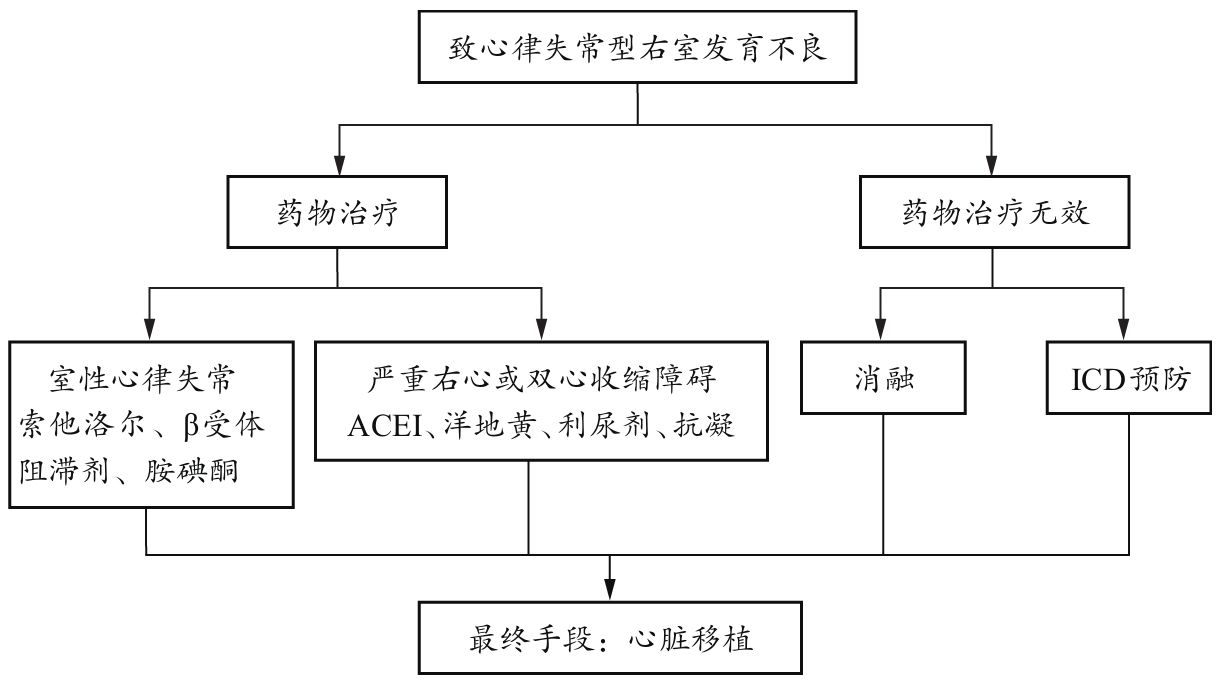
\includegraphics{./images/Image00081.jpg}
 \captionsetup{justification=centering}
 \caption{致心律失常右室发育不良的治疗程序}
 \label{fig2-13-2}
  \end{figure} 

【治疗方案】 治疗目标是控制心律失常、预防猝死。可使用索他洛尔、β受体阻滞剂或钙通道阻滞剂以控制室性心律失常;也可选择导管消融和外科手术切除右室病灶;植入ICD或心脏移植可提高长期生存率。

【疗效观察与随访】 参见扩张型心肌病。

预后不定,猝死为主要死亡原因,且多见于年轻人。经正规治疗,预后一般较好,死亡率2\%左右,ARVC患者左室功能尚好,发生室速时血流动力学耐受较好。

【治疗经验与解析】

1.
由于本病病因未明,防治较困难。临床确诊病例后,可动员患者家属进行检查,以及早治疗,降低风险。

2. 索他洛尔和胺碘酮:单用或β受体阻滞剂联用最为有效。

3. 导管消融成功率60\%\textasciitilde{}90\%,单术后室速复发率约60\%。

4.
对于有室速或室颤反复发作患者,首选ICD,但对右室壁薄弱者,植入ICD有心室穿孔危险。

\subsection{特异性心肌病}

特异性心肌病(specific
cardiomyopathies)是指伴有特异性心脏病或特异性系统性疾病的心肌疾病。包括缺血性心肌病、瓣膜性心肌病、高血压性心肌病(有左心室肥大伴扩张型或限制型心肌病心力衰竭的特点)、炎症性心肌病(有特异性自身免疫性及感染性)、代谢性心肌病(如糖原累积症、糖脂质变性、营养物质缺乏,如钾代谢异常和镁缺乏等)、内分泌性心肌病(如甲状腺功能亢进或减退)、全身疾病所致(结缔组织病、白血病等)、肌营养不良、神经肌肉病变、过敏及中毒反应(乙醇、儿茶酚胺、蒽环类药物、照射等)、围生期心肌病等。

本节重点介绍围生期心肌病、酒精性心肌病、药物中毒性心肌病及克山病(地方性心肌病)。

{(一)围生期心肌病}  围生期心肌病(peripartal
cardiomyopathy)是指既往无心脏病的妊娠末期(分娩前1个月)或产后(妊娠后5个月)女性,出现呼吸困难、血痰、肝大、水肿等心力衰竭症状,酷似扩张型心肌病者。可有心室扩大,附壁血栓。其中,体循环或肺循环栓塞的发生率较高,多发生在30岁左右的经产妇。

【治疗方案】

1.
一般治疗 围生期心肌病伴心功能不全者需绝对卧床休息3\textasciitilde{}6个月。对病情危重者应中止哺乳。另外还需限盐、适当吸氧。

2.
药物治疗 可使用利尿药、ACE抑制剂和血管扩张剂、β受体阻滞剂、钙通道阻滞剂、洋地黄等。对有栓塞史应使用抗凝剂并治疗有风险的心律失常。应采取避孕或绝育措施。适当补充维生素B{1}
100mg肌内注射,每日1次。贫血者可适量成分输血及补充铁剂。还可使用改善心肌代谢药物。

【疗效观察与随访】 参见扩张型心肌病。

多数经治疗后心肌重构逆转。少数患者死于心力衰竭、肺栓塞、恶性心律失常猝死。

【治疗经验与解析】

1. 应早期诊断、及时治疗,同时需使患者安静、增加营养、补充维生素类药物。

2. ACEI有致畸作用,妊娠期禁用,可用硝酸盐类代替,分娩后应视为重要药物。

3.
分娩前可使用肝素、分娩后使用华法林抗凝治疗可使左室射血分数\textless{}35\%的患者获益。

4.
围生期心肌病心肌损害显著,对洋地黄药物敏感,易发生洋地黄中毒,应严密监测。

{(二)酒精性心肌病}  酒精性心肌病(alcoholic
cardiomyopathy)者多为长期且每日大量饮酒,出现酒精依赖症者,临床表现与扩张型心肌病相似。X线示心影扩大,心胸比\textgreater{}55\%。心电图左心室肥大较多见,可伴有各型心律失常。超声心动图或左心室造影示心室腔扩大,射血分数降低。如能排除其他心脏病,且有大量饮酒史(纯乙醇量约125ml/d,即每日啤酒约4瓶或白酒150g),持续10年以上即应考虑本病。

【治疗方案】

1. 早期诊断、早期戒酒。

2.
心力衰竭者,卧床休息,低盐、高营养、高蛋白饮食,可使用ACE抑制剂、洋地黄制剂,利尿剂。适当补镁,大量补充B族维生素。

3. 心律失常者,首选地尔硫䓬
或维拉帕米。

【疗效观察与随访】 参见扩张型心肌病。

本病多伴有高脂血症及高铁血红蛋白血症,易致血栓形成,容易猝死。能早期、长期持续戒酒者预后良好。

【治疗经验与解析】 本病一般不予华法林抗凝,另外创伤或肝功能障碍可引起抗凝过度导致出血。

{(三)克山病}  克山病(Keshan disease,KD)亦称地方性心肌病(endemic
cardiomyopathy,ECD),是在我国发现的一种原因不明的心肌病。1935年在黑龙江省克山县发现此病,因地命名为克山病。此后在黑、吉、辽、蒙、晋、冀、鲁、豫、陕、甘、川、滇、藏、黔、鄂等15个省、自治区的县均有发现。本病全部发生在低硒地区,并有环境卫生差、易有病毒感染为其特点。1980年后由于农村改革开放、人民生活水平的提高,环境卫生的改善,急性克山病已灭迹,遗留下来的慢性病例均类似扩张型心肌病,在克山病死亡病例的尸检心肌标本及患者心内膜心肌活检标本中,经病毒分离或病毒核酸检测多发现与肠道病毒感染有关,缺硒是参与病毒感染致本病发生的重要因素。病理改变主要是心肌实质性变性、坏死和纤维化,心脏呈肌源性普遍扩张,心壁通常不增厚。临床上将克山病分为急性、亚急性、慢性和潜在性。目前主要为慢性克山病,其临床表现、X线、心电图、超声心动图及化验检查均类似扩张型心肌病。

【治疗方案】

1. 防治原则 在缺硒地区需常年口服亚硒酸钠(Na{2} SeO{3}
),每10日口服1次,成人每次4mg。提高生活水平,调整饮食结构,改善水源,人畜饮水分开。

2. 有心力衰竭者 按扩张型心肌病治疗。

3. 休克治疗

(1)大剂量维生素C疗法:10\%\textasciitilde{}12.5\%维生素C注射液5\textasciitilde{}10g加入20\%\textasciitilde{}50\%葡萄糖液20ml中直接静脉注射。2\textasciitilde{}4小时后视病情变化重复相同剂量1\textasciitilde{}2次。第1日可达30g以上,休克缓解后每日静脉注射5g,3\textasciitilde{}5日后停药。小儿用量每次3\textasciitilde{}5g。

(2)补液扩容:静脉缓慢推注5\%葡萄糖盐水200ml、低分子右旋糖酐或生理盐水。

(3)亚冬眠疗法:适用于烦躁不安者与小儿。静脉注射或肌内注射氯丙嗪25mg、异丙嗪25mg、哌替啶50mg(小儿各为0.5\textasciitilde{}1.0mg/kg),或静脉注射地西泮每次20mg(小儿每次0.25\textasciitilde{}0.5mg/kg)。

【疗效观察与随访】 参见扩张型心肌病。

急性型如果能早期就地合理抢救,临床治愈率可达85\%以上,有20\%左右转为慢性,死亡多为心源性休克或猝死。亚急性、慢性患者心脏明显增大伴有严重心律失常者预后差。

【治疗经验与解析】 急性心功能不全出现心源性休克并发室性心律失常或各种类型房室传导阻滞者,多予大剂量维生素C静脉注射或扩容及亚冬眠疗法后,随休克缓解而逐渐消失,一般不需要使用抗心律失常药。


\section{血管疾病}

\subsection{主动脉夹层}

主动脉夹层(aortic
dissection)系主动脉内的血液经内膜撕裂口流入囊样变性的中层,形成夹层血肿,随血流压力的驱动,逐渐在主动脉中层内扩展,是主动脉中层的解离过程。临床特点为急性起病,突发剧烈疼痛、休克和血肿压迫相应的主动脉分支血管时出现的脏器缺血症状。

【治疗程序】 如图\ref{fig2-14-1}所示。

\begin{figure}[!htbp]
 \centering
 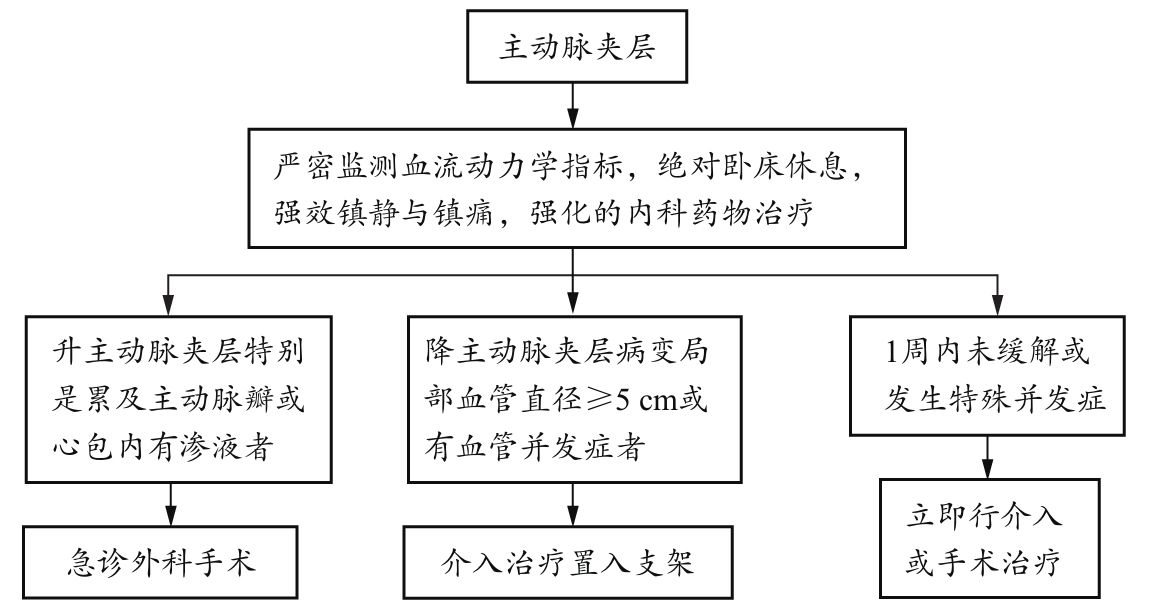
\includegraphics{./images/Image00082.jpg}
 \captionsetup{justification=centering}
 \caption{主动脉夹层的治疗程序}
 \label{fig2-14-1}
  \end{figure} 

【治疗方案】

1.
即刻处理 严密监测血流动力学指标,包括血压、心率、心律;凡有心衰或低血压者还应监测中心静脉压、肺毛细血管嵌压和心排血量。

绝对卧床休息,强效镇静与镇痛,必要时静脉注射较大剂量吗啡。

2.
随后的治疗决策应按以下原则:①急性患者无论是否采取介入或手术治疗均应首先给予强化内科药物治疗。②Deback夹层Ⅰ型、Ⅱ型波及主动脉瓣或心包内有渗液者宜急诊外科手术。③降主动脉夹层急性期病情进展迅速,病变局部血管直径≥5cm或有血管并发症者应争取介入治疗置入支架(动脉腔内隔绝术)。夹层范围局限无特殊血管并发症时,可试行内科药物保守治疗,若1周内未缓解或发生特殊并发症:如血压控制不佳、疼痛顽固、夹层扩展或破裂,出现神经系统损害或膈下大动脉分支受累等,应立即行介入或手术治疗。

3. 内科药物治疗

(1)降压:迅速将收缩压降至\textless{}100\textasciitilde{}120mmHg或更低,可静脉滴注硝普钠,开始时以50mg/500ml浓度每分钟10\textasciitilde{}25μg速率静脉滴注,使用硝普钠必须密切观察血压,根据血压水平仔细调节滴注速率。停止滴注后,作用仅维持3\textasciitilde{}5分钟。硝普钠在通常剂量下不良反应轻微,有恶心、呕吐、肌肉颤动。滴注部位如药物外渗可引起局部皮肤和组织反应。硝普钠在体内红细胞中代谢产生氰化物,长期或大剂量使用应注意可能发生硫氰酸中毒,尤其在肾功能损害者。

(2)β受体阻滞剂:减慢心率至60\textasciitilde{}70次/分,以防止夹层进一步扩展。β受体阻滞剂经静脉给药作用更快。美托洛尔注射液5mg,用葡萄糖溶液稀释后,缓慢静脉注射,如病情需要可相隔10分钟重复注射。美托洛尔口服片,每次剂量一般不超过50mg,每日2\textasciitilde{}3次。

4.
介入治疗 以导管介入方式在主动脉内置入带膜支架,压闭撕裂口,扩大真腔,治疗主动脉夹层。目前,此项措施已成为治疗大多数降主动脉夹层的优选方案。

5. 外科手术治疗 修补撕裂口,排空假腔或人工血管移植术。

【疗效观察与随访】

1.
观察指标 临床症状与体征、血压、心电图、超声心动图、X线胸片、主动脉造影等。

2.
疗效判定 缓解:经急诊处理后,疼痛减轻甚至消失,心率恢复正常范围,心电图改善,血压恢复正常范围。目前常涉及手术或介入治疗,疗效更好。

3.
随访 紧急处理后,特别是术后、介入治疗后,应定期复查心电图,密切观察病情变化。

【治疗经验与解析】

1.
本病未经治疗死亡率极高,以下因素可影响预后:①夹层发生的部位,愈在主动脉远端预后愈好,DebackⅢ型较Ⅱ型好。②诊断及处理越及时预后越好。③合理选择有效的治疗方案如药物、介入或手术。④夹层内血栓形成可防止夹层向外膜破裂,避免内出血的危险。

2. 介入治疗是当前治疗大多数降主动脉夹层的优选方案。

\subsection{多发性大动脉炎}

多发性大动脉炎(Takayasu
arteritis,TA)是指累及主动脉及其主要分支的慢性非特异性炎症,引起的不同部位动脉狭窄或闭塞,出现相应部位缺血表现,少数也可引起动脉扩张或动脉瘤。

【治疗方案】

1.
活动期治疗 如有感染积极控制感染。对活动期患者可用泼尼松(龙)15\textasciitilde{}60mg/d,病情好转后递减,直至病情稳定,5\textasciitilde{}15mg/d维持。对糖皮质激素疗效不佳者可与免疫抑制剂合用,常用环磷酰胺,每日1\textasciitilde{}2mg/kg。

2. 稳定期治疗

(1)血管扩张药物:烟酸50\textasciitilde{}100mg,每日3次;盐酸酚苄明10\textasciitilde{}20mg,每日2\textasciitilde{}3次;卡托普利25\textasciitilde{}50mg,每日3次;地巴唑10mg,每日3次。

(2)抗血小板聚集药物:阿司匹林100mg,每日1次。

(3)改善微循环药物:低分子右旋糖酐500ml或加入丹参20ml中静脉滴注。

3.
手术治疗 对静止期患者,因重要血管狭窄、闭塞,影响脏器供血可考虑手术治疗,如介入治疗、人工血管重建术、内膜血栓清除术、肾切除术、血管搭桥术等。

【疗效观察与随访】

1.
观察指标 临床症状与体征、血管超声、血管造影、血沉等。①急性炎症期应观察治疗前后患者有无发热、心悸、盗汗、乏力、食欲不振和关节酸痛等非特异性炎症症状,体检有无结节性红斑、血管神经性水肿和关节肿痛等表现。②慢性血管闭塞期因出现血管狭窄、闭塞,相应的脏器和组织的症状、体征,观察治疗前后的转归。③另外可监测血常规、血沉、免疫球蛋白、彩色多普勒、HRCT、MRI、DSA等变化。

2. 疗效判定 好转:症状减轻,脉搏恢复至正常范围。

3. 随访 治疗后密切观察症状变化,定期检查血管超声。

【治疗经验与解析】 本病多缓慢起病,受累动脉易形成侧支循环,因此只要不累及重要脏器供血,多数患者预后良好。5年生存率为93.8\%,10年生存率为90.9\%,常见死亡原因为脑出血,其次为手术并发症、肾衰竭及心力衰竭。


\section{人工心脏起搏和心脏电复律}

\subsection{人工心脏起搏}

心脏起搏器通过脉冲发生器,用特定频率的脉冲电流,经过起搏电极刺激心脏,使之激动收缩,即模拟正常心脏的冲动形成和传导,以治疗某些心律失常所致的心脏功能障碍。目前心脏起搏的适应范围由单纯治疗缓慢性心律失常,扩展到治疗快速性心律失常、慢性心力衰竭、肥厚型梗阻性心肌病(HOCM)、长QT综合征等。

【起搏器选择顺序】

1. 窦房结功能障碍患者起搏器选择顺序(图\ref{fig2-15-1})

\begin{figure}[!htbp]
 \centering
 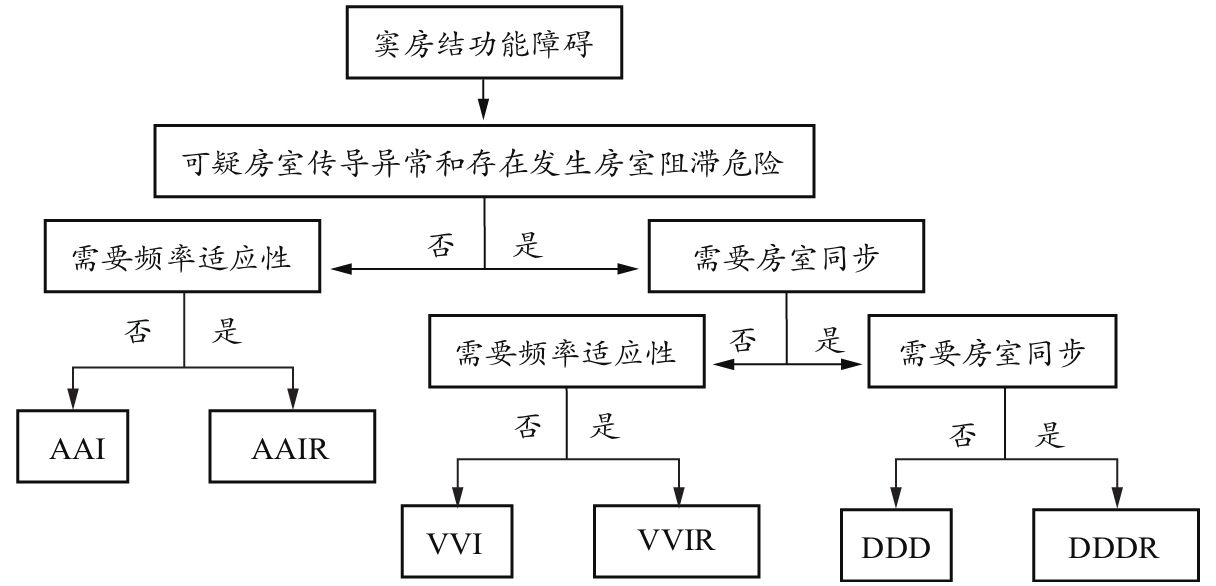
\includegraphics{./images/Image00083.jpg}
 \captionsetup{justification=centering}
 \caption{窦房结功能障碍患者起搏器选择顺序}
 \label{fig2-15-1}
  \end{figure} 

2. 房室传导阻滞患者起搏器选择顺序(图\ref{fig2-15-2})

\begin{figure}[!htbp]
 \centering
 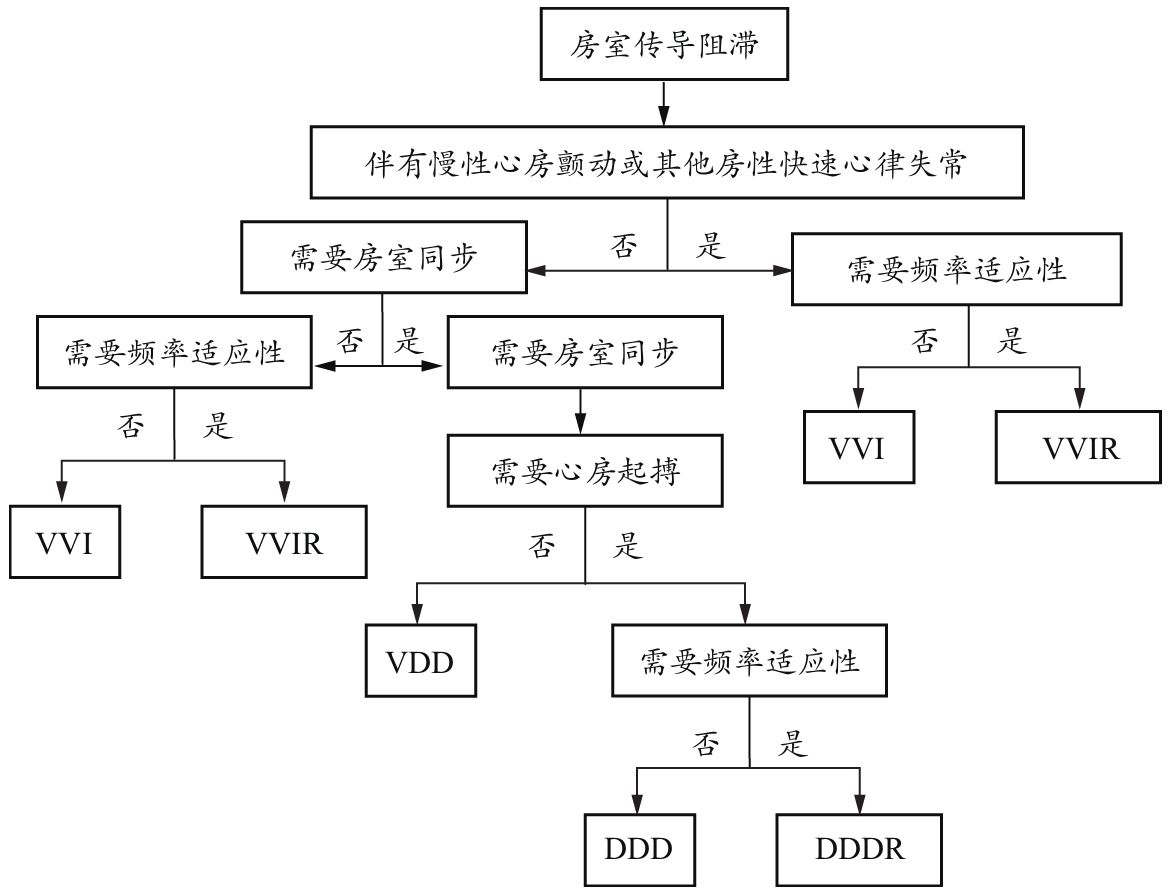
\includegraphics{./images/Image00084.jpg}
 \captionsetup{justification=centering}
 \caption{房室传导阻滞患者起搏器选择顺序}
 \label{fig2-15-2}
  \end{figure} 

【治疗方案】 对于具备适应证的患者,安装临时性起搏器或者永久性起搏器。

1. 临时性起搏器适应证

(1)治疗方面:有生命威胁的心律失常时,维持适当的心率。

阿-斯综合征发作:房室传导阻滞、窦房结功能衰竭等各种原因引起的心脏停搏所导致的阿-斯综合征发作,是紧急临时起搏的绝对指征。

急性心肌梗死、急性心肌炎、药物中毒、电解质紊乱等疾病时出现的缓慢心律失常。

心脏直视手术引起的房室传导阻滞。

(2)诊断方面:作为某些临床诊断及电生理检查的辅助手段。例如判断:①预激综合征类型;②房室结功能;③窦房结功能;④折返性心律失常;⑤抗心律失常药物效果。

(3)预防方面:①心脏起搏传导系统功能不全患者拟施行大手术、心血管造影检查或心律转复治疗时可安置临时起搏器保护。②心律不规则的患者在安置永久起搏器之前,可先作临时起搏以保证安全。③作为更换新的永久性起搏器时的过渡。

2. 永久性起搏器的适应证 植入性心脏起搏器(implantable
Pacemaker)治疗的适应证主要是症状性心动过缓(symptomatic
bradycardia),包括直接由于心率过于缓慢导致心排出量下降,重要脏器及组织尤其大脑供血不足而产生的一系列症状,如一过性晕厥、近似晕厥、头晕黑蒙等;长期心动过缓引起全身性症状,如疲乏、运动耐量下降以及慢性心力衰竭等。根据2010年中华医学会心电生理和起搏分会(CSPE)制定的“植入性心脏起搏器治疗---------目前认识和建议(2010年修订版)”,起搏器植入的主要的适应证如下:

(1)窦房结功能障碍:①窦房结功能障碍表现为症状性心动过缓,包括频繁的有症状的窦性停搏。②因窦房结变时性不良而引起症状者。③由于某些疾病必须使用某些类型和剂量的药物治疗,而这些药物又可引起或加重窦性心动过缓并产生症状者。

(2)成人获得性完全性房室阻滞:任何阻滞部位的三度和高度房室阻滞伴下列情况之一者:①有房室阻滞所致的症状性心动过缓(包括心力衰竭)或继发于房室阻滞的室性心律失常。②需要药物治疗的其他心律失常或其他疾病,而所用药物可导致症状性心动过缓。③虽无临床症状,但业已证实心室停搏≥3秒或清醒状态时逸搏心率≤40次/分钟,或逸搏心律起搏点在房室结以下者。④射频消融房室交界区导致的三度和高度房室阻滞。⑤心脏外科手术后发生的不可逆性房室阻滞。⑥神经肌源性疾病(肌发育不良、克塞综合征等)伴发的房室阻滞、无论是否有症状,因为传导阻滞随时会加重。⑦清醒状态下无症状的房颤和心动过缓者,有1次或更多至少5秒的长间歇。

任何阻滞部位和类型的二度房室阻滞产生的症状性心动过缓。

无心肌缺血情况下运动时的二度或三度房室阻滞。

(3)慢性双分支和三分支阻滞:①双分支或三分支阻滞伴高度房室阻滞或间歇性三度房室阻滞。②双分支或三分支阻滞伴二度Ⅱ型房室阻滞。③交替性束支阻滞。

(4)心肌梗死急性期后:①急性心肌梗死后持续存在的希氏浦肯野系统内的二度房室阻滞伴交替性束支阻滞,或希氏浦肯野系统内或其远端的三度房室阻滞。②房室结以下的一过性高二度或三度房室阻滞,伴束支阻滞者。如果阻滞部位不明确则应进行电生理检查。③持续和有症状的二度或三度房室阻滞。

(5)颈动脉窦过敏综合征及神经介导性晕厥:反复发作的由颈动脉窦刺激或压迫导致的心室停搏\textgreater{}3秒所致的晕厥。

3. 在某些特殊情况的心脏起搏治疗

(1)肥厚梗阻型心肌病(HOCM):HOCM合并符合窦房结功能不良和(或)房室阻中的主要适应证的各种情况。

(2)收缩性心力衰竭患者心脏再同步治疗:同时满足以下条件者可植入有(无)ICD功能的CRT:①缺血性或非缺血性心肌病;②充分抗心力衰竭药物治疗后,心功能NYHAⅢ级以上;③窦性心律;④LVEF≤0.35;⑤QRS时限≥120毫秒。

(3)长QT综合征:长间歇依赖性持续性室速,可合并或无长QT间期,起搏治疗证明有效。

(4)心脏移植起搏适应证:预计难以恢复的持续性或症状性缓慢心律失常患者,以及其他符合上述起搏器植入主要适应证患者。

4. 起搏器的选择方案

(1)VVI起搏器:按需型心室起搏(VVI)为非生理性起搏模式,为非房室同步性起搏,但在我国目前经济条件下是临床应用较为广泛的一种起搏模式。适用于窦房结功能障碍及伴有慢性心房颤动或其他快速房性心律失常伴房室阻滞,起搏时不必保持房室同步性患者。VVI起搏干扰正常房室顺序收缩,不能够改善心功能。

(2)AAI起搏器:AAI是生理起搏的一种模式,对于窦房结功能障碍而房室结功能良好患者,这种起搏方式最为适宜。对于有房室传导异常可能和慢性房性快速性心律失常(心房颤动、心房扑动、房性心动过速等)不宜选用。

(3)DDD起搏器:DDD起搏器又称房室全能型起搏器,既能起搏又能感知心房和心室。由于其工作模式齐全以及自动模式转换功能,因此DDD起搏器可根据需要以各种模式进行工作。其优点在于心房心室顺序收缩,可提高心排血量;起搏频率可随自身窦性心房率进行调整,增加患者运动耐力。

(4)频率应答起搏器:频率应答起搏器的起搏频率并非固定不变的,它能够根据人体活动或代谢变化而自动调节。主要应用于心脏变时功能不良患者。

5. 注意事项

(1)通过体表心电图和程控仪遥测获取心电信息:①确定患者是自身心律还是起搏心律;是窦性心律还是房颤心律,目前起搏模式和感知状况。②确定起搏器在相应的心腔能够有效夺获及感知状况。

(2)通过查询程控仪相应模块获取电池状态和起搏器使用寿命。

(3)有频率应答功能的起搏器,通过程控仪的有关信息评估作为优化感知器驱动频率响应的电极导线的工作情况。

(4)有快速性心律失常诊断功能的双腔起搏器,通过查询程控仪的相关信息,获取发生快速性心律失常发作情况,起搏器工作模式自动转换情况,对相关参数作必要调整。

(5)随访频度:具体随访的时间表应该由提供起搏器随访的医务人员做出。建议患者应在植入起搏器后1\textasciitilde{}3个月内随访1次,然后每6\textasciitilde{}12个月随访1次。接近起搏器担保期时,每3\textasciitilde{}6个月随访1次。

\subsection{心脏电复律}

心脏电复律和电除颤是用一定强度电流作用于心脏,使全部或大部分心肌瞬时除极,然后由自律性最高的起搏点(通常为窦房结)重新主导心脏节律,从而使多种快速心律失常转变为窦性心律,是迅速终止伴有血流动力学障碍的异位快速心律失常有效方法。

【适应证】

1. 体外电复律和电除颤的适应证

(1)同步电复律:电复律是以自身的心电信号作为触发标志,同步瞬间高能放电终止某些异位快速心律失常,如心房颤动、心房扑动,对药物无效的且伴有血流动力学障碍的室上速和室速。

室速:室性心动过速经药物治疗无效或临床情况严重,如伴急性心肌梗死、心力衰竭、休克、阿-斯综合征等需紧急处理者,应及早进行同步直流电复律。所需能量100\textasciitilde{}200J。

阵发性室上性心动过速常规物理和药物治疗无效而伴有明显血流动力学障碍者,可考虑同步直流电复律。所需能量为50\textasciitilde{}100J。

心房颤动、心房扑动:直流电转复心房扑动主要适用于发作时心室率很快,伴有血流动力学紊乱或伴胸痛、心功能不全等。具有能量低、成功率高、速度快的特点,一般推荐心房扑动的能量50J、房颤100\textasciitilde{}200J。

(2)非同步电除颤:心室颤动与心室扑动是非同步电除颤的绝对适应证,此时心脏的有效收缩消失,血液循环处于停顿状态,必须立即实施电除颤。距离心房颤动、心房扑动发生时间越短,成功几率越大。

2. 埋藏式心脏复律除颤器

(1)心源性猝死的二级预防:主要针对已经发生过室性快速心律失常(包括VF和VT)所致的心脏骤停、确证有过VT或VF等重大事件或伴有明显器质性心脏病并可诱发室性心律失常的晕厥人群。①心室颤动或血流动力学不稳定的持续室速引起的心脏骤停存活者,经过仔细评估明确原因且完全排除可逆因素后。②合并自发持续室速的器质性心脏病患者,无论血流动力学是否稳定。③不明原因的晕厥患者,伴随电生理检查诱发的临床相关血流动力学不稳定持续室速或室颤。④心肌梗死所致非持续室速,LVEF\textless{}40\%且电生理检查诱发出心室颤动或持续室速。

(2)心源性猝死一级预防:针对已发生过心肌梗死同时左心室射出功能损伤及缺血性(非心肌梗死)或非缺血性心肌病变,心力衰竭NYHA心功能分级为Ⅱ\textasciitilde{}Ⅲ级,且LVEF≤35\%的人群。①心肌梗死所致LVEF\textless{}35\%,且心肌梗死40日以上,NYHAⅡ或Ⅲ级患者。②NYHAⅡ或Ⅲ级,LVEF≤35\%的非缺血性心肌病患者。③心肌梗死所致LVEF≤30\%,且心肌梗死40日以上,NYHAⅠ级患者。

【注意事项】 主要是针对植入埋藏式心脏复律除颤器的患者,除颤器应定期监测。

1.
加强监测 包括对系统的功能进行监护;优化性能以使系统能够发挥最佳的临床功效并达到最长的使用年限;减少并发症的发生;对系统器件更换进行预测;确保对临床发生问题的适时干预;患者的跟踪、教育和支持;系统记录的维护。

2.
注意随访 ICD随访必须根据患者的临床状态进行个性化的随访,应由受过专门训练的心脏电生理医生进行操作。植入后每1\textasciitilde{}4个月随访1次,具体随访间隔根据ICD的类型以及患者的临床状况决定。如有放电事件发生应及时到医院检查。

3. 有血栓栓塞风险患者电复律时应慎重,应进行有效的抗凝治疗。

4.
对于心室颤动的可逆原因已明确患者,如急性心肌梗死、冠脉痉挛或电解质紊乱所发生的快速性室性心律失常;无诱发或自发室速且准备接受冠状动脉搭桥的冠心病患者;因预激综合征伴发房颤恶化为室颤的患者等不宜植入埋藏式心脏复律除颤器(ICD)。

5.
由于大部分患者是先出现室速,进而恶化为室颤,抗心动过速起搏(antitachycardial
pacing,ATP)可以有效地终止室速,这样一方面可以减少放电导致患者痛苦,提高ICD植入的耐受性,另一方面可以减少放电量,延长ICD寿命。在应用ICD治疗时,应根据患者室速发作情况,尽量应用抗心动过速起搏终止室速发作。